\documentclass[letterpaper, 12pt]{article}
\usepackage[top = 1.6cm, left = 2cm, right = 2cm ]{geometry}
\usepackage[pdftex]{graphicx}
\usepackage{amsmath}
\usepackage{tikz}
\usepackage[utf8]{inputenc}
\usepackage[T1]{fontenc}
\usepackage{float}
\usepackage{epigraph}
\usepackage{fancyhdr}
\usepackage{xcolor}
\usepackage{color,soul}

\def\changemargin#1#2{\list{}{\rightmargin#2\leftmargin#1}\item[]}
\let\endchangemargin=\endlist 

\newcommand{\newlinealinea}{
	~\\ \hspace*{0.5cm}}
\newcommand{\alinea}{
\hspace*{0.3cm}}
\newcommand{\alinealong}{
\hspace*{1.1cm}}
\newcommand{\alignparagraph}{
\hspace*{0.6cm}}


\makeatletter
\@addtoreset{section}{part}
\makeatother  

\definecolor{darkgreen}{rgb}{0., 0.66, 0.}


\newcommand{\red}[1]{
	\textcolor{red}{#1}
}
\newcommand{\green}[1]{
	\textcolor{darkgreen}{#1}
}

\newcommand{\myul}[1]{
	\underline{\smash{#1}}
}

\newcommand{\point}{$\bullet\ $}


\renewcommand*\sfdefault{phv}
\renewcommand*\rmdefault{ppl}

\renewcommand\epigraphflush{flushright}
\renewcommand\epigraphsize{\normalsize}
\setlength\epigraphwidth{0.7\textwidth}

\definecolor{titlepagecolor}{cmyk}{1,.60,0,.40}

\DeclareFixedFont{\titlefont}{T1}{phv}{\seriesdefault}{n}{0.375in}

\makeatletter                       
\def\printauthor{%                  
    {\large \@author}}             
\makeatother
   
\pagestyle{fancy}
\lhead{Anthony Rouneau}
\rhead{MAB1 Sciences Informatiques}
\cfoot{\thepage}

% The following code is borrowed from: http://tex.stackexchange.com/a/86310/10898

\newcommand\titlepagedecoration{%
\begin{tikzpicture}[remember picture,overlay,shorten >= -10pt]

\coordinate (aux1) at ([yshift=-70pt]current page.north east);
\coordinate (aux2) at ([yshift=-460pt]current page.north east);
\coordinate (aux3) at ([xshift=-6cm]current page.north east);
\coordinate (aux4) at ([yshift=-150pt]current page.north east);

\begin{scope}[titlepagecolor!40,line width=12pt,rounded corners=12pt]
\draw
  (aux1) -- coordinate (a)
  ++(225:5) --
  ++(-45:5.1) coordinate (b);
\draw[shorten <= -10pt]
  (aux3) --
  (a) --
  (aux1);
\draw[opacity=0.6,titlepagecolor,shorten <= -10pt]
  (b) --
  ++(225:2.2) --
  ++(-45:2.2);
\end{scope}
\draw[titlepagecolor,line width=8pt,rounded corners=8pt,shorten <= -10pt]
  (aux4) --
  ++(225:0.8) --
  ++(-45:0.8);
\begin{scope}[titlepagecolor!70,line width=6pt,rounded corners=8pt]
\draw[shorten <= -10pt]
  (aux2) --
  ++(225:3) coordinate[pos=0.45] (c) --
  ++(-45:3.1);
\draw
  (aux2) --
  (c) --
  ++(135:2.5) --
  ++(45:2.5) --
  ++(-45:2.5) coordinate[pos=0.3] (d);   
\draw 
  (d) -- +(45:1);
\end{scope}
\end{tikzpicture}%
}

\begin{document}
\begin{titlepage}

\noindent
%\begin{changemargin}{3cm}{3cm}

%\epigraph{Pure mathematics is on the whole distinctly more useful than applied.\\
%For what is useful above all is technique, and mathematical technique\\
%is taught mainly through pure mathematics.}%
%{\textit{London 1941}\\ \textsc{G. H. Hardy}}

%\end{changemargin}


\newgeometry{bottom = 2cm, top = 2.5cm}
\begin{center}

\includegraphics[scale=1.2]{Images/UMONS}\\
\vspace*{0.3cm}

\includegraphics[scale=0.23]{Images/FS_Logo}\\
\vspace*{2.5cm}
\titlefont Traitement de la parole:\\Notes de cours\par
\end{center}
\vspace*{3cm}
\hfill
\begin{minipage}{0.18\linewidth}
  \begin{flushright}
   \rule{0.5pt}{60pt}
  \end{flushright}
\end{minipage}
\begin{minipage}{0.8\linewidth}
\begin{flushleft}
\textsf{\textbf{Notes écrites par:}} Anthony Rouneau\\
\textsf{\textbf{Section:}} 1$^{er}$ Bloc Master en Sciences Informatiques
%
\end{flushleft}
\end{minipage}
\vspace*{\fill}
\begin{center}
Faculté des Sciences $\bullet$ Université de Mons $\bullet$ Place du Parc 20 $\bullet$ B-7000 Mons
\end{center}
\titlepagedecoration
\end{titlepage}

\newgeometry{top = 3cm, left = 2cm, right = 2cm}

%%%%%%%%%%%%%%%%%%%%%%%%%%%%%%%%%%%%%%%%%%%%%%%%%%%%%%%%%%%%%%%%%%%%%%%%%%%%%%%%%%%%%%%%%%%%%%%%%%%%%%%
%										      Compétences											  %
%%%%%%%%%%%%%%%%%%%%%%%%%%%%%%%%%%%%%%%%%%%%%%%%%%%%%%%%%%%%%%%%%%%%%%%%%%%%%%%%%%%%%%%%%%%%%%%%%%%%%%%

\part{Compétences requises pour l'examen}
\section{Introduction to speech}
	\subsection{An Introductory Course on Speech Processing}
	\begin{itemize}
		\setlength{\itemsep}{0pt}		
		\setlength{\parskip}{0pt}		
		\setlength{\parsep}{0pt}	
		\item Dissocier le traitement de la parole du traitement du signal.
		\item Justifier par une raison valable la complexité du signal de parole.
		\item Citer les principales sciences et techniques concernées par le traitement de la parole.
		\item Identifier les domaines de recherche du traitement de la parole.
		
	\end{itemize}
	\subsection{Acoustics}
	\begin{itemize}
		\setlength{\itemsep}{0pt}		
		\setlength{\parskip}{0pt}		
		\setlength{\parsep}{0pt}	
		\item Nommer les 7 profils de spécialistes travaillant en traitement de la parole.
		\item Expliquer en quoi consiste le travail d'analyse d'un acousticien.
		\item Définir ce qu'est un audiogramme, comment on l'obtient et préciser quels traits 
		acoustiques il permet de mettre en évidence.
		\item Différencier sur un audiogramme les signaux voisés des signaux non voisés.
		\item Décrire le résultat d'une analyse de Fourier et préciser quels traits acoustiques elle 
		permet de mettre en évidence.
		\item Caractériser ce qu'est un formant.
		\item Différencier formant et fondamental.
		\item Décrire le principe de construction d'un spectrogramme, préciser son utilité et son utilisation.
		\item Dessiner une courbe typique d'intonation et en expliquer l'utilité.
		\end{itemize}
	\subsection{Phonetics}
	\begin{itemize}
		\setlength{\itemsep}{0pt}		
		\setlength{\parskip}{0pt}		
		\setlength{\parsep}{0pt}	
		\item Donner un diagramme schématique du conduit vocal et des cordes vocales et en décrire le 
		fonctionnement.
		\item Citer et détailler les principaux modes de classification articulatoires en soulignant leurs 
		différences de principes.
		\item Présenter par un exemple la classification par lieux d'articulation.
		\item Donner un exemple des caractéristiques complémentaires de sons exploitées en phonétique.
		\item Expliquer le principe qui a conduit à l'élaboration de l'alphabet phonétique international.
		\item Établir le lien entre la description acoustique et phonétique de la parole.
		\item Définir ce que l'on entend par « niveau de description segmental », par opposition au niveau
		« suprasegmental ».
		\item Citer les trois caractéristiques globalisées par le terme « prosodie ».
	\end{itemize}
	\subsection{Phonology}
	\begin{itemize}
		\setlength{\itemsep}{0pt}		
		\setlength{\parskip}{0pt}		
		\setlength{\parsep}{0pt}	
		\item Différencier les niveaux de description de la parole dépendant de la langue des niveaux qui n'en 
			dépendent pas.
		\item Donner la définition de phonème et le nombre de phonèmes dans la langue française.
		\item Donner un exemple d'allophone.
		\item Citer et définir sur base d'un exemple (à donner) la principale distinction entre phonème et son (ou 
			phone).
		\item Commenter l'affirmation suivante : « Lorsqu'on connaît le fossé qui sépare la représentation acoustique 
			de la parole de son niveau phonologique, la communication parlée tient du miracle ».
		\item Justifier l'expression « C'est du chinois ! » du point de vue de la phonologie.
		\item Définir la coarticulation et en justifier son impact en traitement de la parole en l'illustrant par un 
			schéma.
	\end{itemize}
	\subsection{Morphology}
	\begin{itemize}
		\setlength{\itemsep}{0pt}		
		\setlength{\parskip}{0pt}		
		\setlength{\parsep}{0pt}	
		\item Donner un ordre de grandeur du nombre de mots d'une langue naturelle (comme la langue française) et du 
			nombre de mots utilisé dans le langage quotidien.
    	\item Définir ce qu'est un morphème et en donner un exemple.
    	\item Citer et expliquer les trois procédés morphologiques fondamentaux d'une langue naturelle.
    	\item Illustrer par deux exemples le fait que chaque langue utilise à sa façon les trois procédés de 
    		transformation morphologique.
	\end{itemize}
	\subsection{Syntax}
	\begin{itemize}
		\setlength{\itemsep}{0pt}		
		\setlength{\parskip}{0pt}		
		\setlength{\parsep}{0pt}	
		\item Donner le but premier de l'analyse syntaxique.
    	\item Distinguer syntaxe et grammaire.
    	\item Nommer le type de grammaires compréhensibles par un ordinateur (en donner un exemple) et la 
    		discipline scientifique qui en découle.
    	\item Justifier pourquoi il est intéressant de réaliser une analyse syntaxique, au delà de la 
    		vérification de la validité syntaxique de la phrase.
	\end{itemize}
	\subsection{Semantics \& Pragmatics}
	\begin{itemize}
		\setlength{\itemsep}{0pt}		
		\setlength{\parskip}{0pt}		
		\setlength{\parsep}{0pt}	
		\item Opposer syntaxe et sémantique.
    	\item Spécifier la base de construction des règles sémantiques.
    	\item Nommer et décrire par un exemple un problème classique de la sémantique. Désigner en une phrase les 
    		caractéristiques de la parole concernées par la pragmatique.
	\end{itemize}
	\subsection{From Source To Receiver}
	\begin{itemize}
		\setlength{\itemsep}{0pt}		
		\setlength{\parskip}{0pt}		
		\setlength{\parsep}{0pt}	
		\item Décrire le fonctionnement de l'oreille et schématiser ses principales parties.
    	\item Justifier l'analogie entre la cochlée et un analyseur spectral.
    	\item Justifier que la psychophysique ait permis de normaliser la transmission de parole sur les canaux 
    		téléphoniques et traduire cette justification par un schéma.
    	\item Donner la définition des courbes isosoniques et les comparer aux courbes de seuil de l'audition et de 
    		seuil de la douleur.
    	\item Décrire le phénomène de masquage auditif et donner un exemple d'impact technologique en traitement de la 
    		parole.
	\end{itemize}
\section{Modeling of the speech signal}
	\subsection{Autoregresive modeling of the speech}
		\begin{itemize}
			\setlength{\itemsep}{0pt}		
			\setlength{\parskip}{0pt}		
			\setlength{\parsep}{0pt}	
			\item Distinguer les deux étapes du processus de mise en œuvre d'un nouveau modèle de la parole.
    		\item Différencier erreurs de modélisation et erreur d'estimation, et montrer que la création d'un modèle 
    			résulte d'un compromis entre ces deux types d'erreurs.
    		\item Citer et caractériser les trois grandes familles de modèles de la parole.
    		\item Présenter le modèle autorégressif de traitement de la parole en réalisant l'analogie avec le système 
    			naturel de production de la parole.
    		\item Donner un schéma de principe du modèle LPC de traitement de la parole, citer ses paramètres et 
    			caractériser leur rôle.
		\end{itemize}
	\subsection{Autoregressive estimation of speech}
		\begin{itemize}
			\setlength{\itemsep}{0pt}		
			\setlength{\parskip}{0pt}		
			\setlength{\parsep}{0pt}	
			\item Expliquer pourquoi la modélisation autorégressive est basée sur un principe de minimisation 
				d'erreur.
		    \item Décrire le système d'équations de Yule-Walker, en expliquer les composantes et justifier sa facilité 
		    	de résolution.
    		\item Préciser l'avantage de l'algorithme de Schur sur celui de Levinson.
		    \item Critiquer un choix de fréquence d'échantillonnage dans l'analyse d'un signal de parole.
    		\item Donner une analyse critique du choix de l'ordre de prédiction pour modéliser la parole.
		\end{itemize}
	\subsection{Extension of the AR model}
		\begin{itemize}
			\setlength{\itemsep}{0pt}		
			\setlength{\parskip}{0pt}		
			\setlength{\parsep}{0pt}	
			\item Expliquer comment on synthétise un signal de parole avec le modèle LPC.
    		\item Préciser les éléments du modèle sur lesquels agir pour améliorer la qualité du signal modélisé.
    		\item Citer deux types de problèmes typiques de l'analyse LPC.
    		\item Définir ce qu'est un anti-formant et préciser son origine dans le système naturel de production de 
    			la parole.
    		\item Préciser l'origine des sons mixtes dans le système naturel de production de la parole.
    		\item Rappeler l'idée de base du modèle MP-LPC.
    		\item Préciser comment estimer un modèle MP-LPC et expliquer la difficulté de cette estimation.
    		\item Rappeler l'idée de base du modèle CELP et citer un problème de ce modèle.
		\end{itemize}
\section{Speech Coding}
	\subsection{Speech Coding}
		\begin{itemize}
			\setlength{\itemsep}{0pt}		
			\setlength{\parskip}{0pt}		
			\setlength{\parsep}{0pt}	
			\item Citer les deux buts fondamentaux du codage d'un signal de parole.
		    \item Expliquer pourquoi les algorithmes traditionnels de compression ne fonctionnent pas pour un fichier 
		    	de parole.
		    \item Donner l'ordre de grandeur du débit binaire minimal d'un signal de parole (en ne considérant que son 
		    	contenu phonétique) et le comparer au débit binaire admissible par une ligne téléphonique.
		    \item Décrire en les illustrant par un schéma, la technique de quantification uniforme et l'erreur de 
		    	quantification qui lui est liée.
		    \item Détailler l'emploi de la technique de quantification uniforme pour un CD audio et calculer le débit 
		    	binaire correspondant.
		    \item Détailler l'emploi de la technique de quantification uniforme pour le codage de parole.
		    \item Expliquer le principe d'une compression selon la loi A et citer une technologie qui l'exploite.
		\end{itemize}
	\subsection{Coders}
		\begin{itemize}
			\setlength{\itemsep}{0pt}		
			\setlength{\parskip}{0pt}		
			\setlength{\parsep}{0pt}	
			\item Schématiser un codeur par prédiction linéaire et commenter son fonctionnement.
		    \item Citer la caractéristique typique de la parole codée en respectant la norme LPC10 et donner 
		    	un exemple d'emploi dans la vie courante.
		    \item Schématiser un codeur MP-LPC et commenter son fonctionnement.
		    \item Justifier la dégradation de la parole lors d'une communication par GSM.
		    \item Schématiser un codeur CELP et commenter son fonctionnement.
		    \item Expliquer l'avantage que procure l'UMTS sur le GSM en ce qui concerne la transmission de la voix.
		\end{itemize}
	\subsection{Conclusion}
		\begin{itemize}
			\setlength{\itemsep}{0pt}		
			\setlength{\parskip}{0pt}		
			\setlength{\parsep}{0pt}	
			\item Positionner sur un schéma qualité/débit les techniques de codage de parole.
		    \item Citer une restriction importante à opérer sur le signal de parole traité, pour espérer 
		    	un jour coder la parole avec un très bas débit (moins de 200 bits/s).
		    \item Prédire l'avenir de la recherche en codage de parole et justifier cette prédiction.
		\end{itemize}
\section{Automatic Speech Recognition}
	\subsection{Automatic Speech Recognition (ASR)}
		\begin{itemize}
			\setlength{\itemsep}{0pt}		
			\setlength{\parskip}{0pt}		
			\setlength{\parsep}{0pt}	
			\item Justifier, sur le plan économique, le développement des systèmes de reconnaissance de parole.
		    \item Donner trois domaines d'application de la reconnaissance de parole, ainsi qu'un exemple 
		    	pratique pour chacun de ces domaines.
		    \item Expliquer pourquoi la coarticulation représente un important défi de la reconnaissance de parole.
		    \item Citer la plus importante faiblesse des systèmes de reconnaissance de parole actuels.
		    \item Citer et définir les deux principaux types de bruit, donner deux exemples par type.
		    \item Donner une idée de ce qu'est l'effet Lombard.
		\end{itemize}
	\subsection{ASR Systems}
		\begin{itemize}
			\setlength{\itemsep}{0pt}		
			\setlength{\parskip}{0pt}		
			\setlength{\parsep}{0pt}	
			\item Énoncer les contraintes qui régissent le choix d'un système de reconnaissance de parole.
		    \item Positionner la complexité d'un système de reconnaissance de parole par rapport à un autre 
		    	en fonction de leurs contraintes.
		    \item Schématiser et commenter les principes de fonctionnement des trois grandes familles 
		    	de reconnaisseurs de parole étudiés depuis les années 60.
		    \item Expliquer quels types de connaissances embarque un système de reconnaissance basée sur 
		    	des modèles statistiques.
		    \item Préciser les contextes d'utilisations respectifs (en fonction des contraintes qui régissent 
		    	le choix d'un système de reconnaissance) de la de la reconnaissance basée sur des modèles et 
		    	de celle basée sur des modèles statistiques.
		\end{itemize}
	\subsection{Instance-based ASR}
		\begin{itemize}
			\setlength{\itemsep}{0pt}		
			\setlength{\parskip}{0pt}		
			\setlength{\parsep}{0pt}	
			\item Préciser le problème de base d'un système de reconnaissance basé sur des exemples et 
				présenter la solution généralement employée.		
		    \item Préciser la notion de distance locale et de distance globale dans le cadre d'un système 
		    	de reconnaissance basé sur des exemples.
         	\item Schématiser la solution la plus adéquate au problème du calcul de la distance globale 
    	    	dans le cadre de la reconnaissance basé sur des exemples, lorsque les mots à 
    	        reconnaître sont longs.
			\item Expliquer conceptuellement l'algorithme DTW.
		\end{itemize}
	\subsection{Model-based ASR}
		\begin{itemize}
			\setlength{\itemsep}{0pt}		
			\setlength{\parskip}{0pt}		
			\setlength{\parsep}{0pt}	
			\item Présenter la classification bayesienne et définir les termes de la règle de Bayes dans le cadre 
				de la reconnaissance basée sur des modèles.
    		\item Développer la règle de Bayes afin d'obtenir une expression exploitable de la probabilité 
    			à posteriori de prononciation d'une phrase, justifier chaque étape de ce développement.
    		\item Citer les probabilités estimées par les modèles acoustique, phonétique et de la langue.
		\end{itemize}
	\subsection{Acoustic Model : Markoov Chain}
		\begin{itemize}
			\setlength{\itemsep}{0pt}		
			\setlength{\parskip}{0pt}		
			\setlength{\parsep}{0pt}	
			\item Décrire le principe des chaînes de Markov.
    		\item  Expliquer pourquoi une chaîne de Markov ne permet pas de calculer directement une probabilité 
    			dans un modèle acoustique en reconnaissance de parole basée sur des exemples.
		\end{itemize}
	\subsection{Acoustic Model : Hidden Markov Model (HMM)}
		\begin{itemize}
			\setlength{\itemsep}{0pt}		
			\setlength{\parskip}{0pt}		
			\setlength{\parsep}{0pt}	
			\item Décrire le fonctionnement des modèles de Markov cachés sur base d'un exemple.
			\item Différencier les probabilités d'émission et de transition dans les modèles de Markov cachés.
			\item Définir en quoi les modèles de Markov cachés sont-ils doublement stochastiques.
			\item Citer et définir les trois types de problèmes à traiter pour utiliser les modèles de Markov cachés.
			\item Citer les deux algorithmes utilisés pour résoudre le problème d'estimation des modèles de 
				Markov cachés.
			\item Illustrer par un exemple l'entraînement d'un modèle de Markov caché.
			\item Énoncer le principe général de l'algorithme EM permettant l'entraînement des modèles de 
				Markov cachés.
		\end{itemize}
	\subsection{Phonetic Model}
		\begin{itemize}
			\setlength{\itemsep}{0pt}		
			\setlength{\parskip}{0pt}		
			\setlength{\parsep}{0pt}	
			\item Citer la technique utilisée dans les modèles phonétique pour calculer la probabilité 
				d'une transcription phonétique étant donné une suite de mots.
			\item Donner un exemple illustrant les limites des modèles phonétiques. 
			\item Préciser comment les modèles phonétiques intègrent un traitement individualisé pour chaque 
				phonème et signaler les avantages de cette technique.
		\end{itemize}
	\subsection{Language Model}
		\begin{itemize}
			\setlength{\itemsep}{0pt}		
			\setlength{\parskip}{0pt}		
			\setlength{\parsep}{0pt}	
			\item Citer et définir les trois problèmes des modèles de la langue.
			\item Exprimer de trois façons différentes la probabilité de prononcer une phrase donnée en fonction 
				des mots qui la composent et commenter l'utilisation de ces expressions dans les modèles de la langue.
			\item Donner une valeur réaliste au nombre n du modèle n-gramme et préciser les conséquences liées 
				à ce choix.
			\item Citer le problème du modèle n-gramme et proposer deux techniques pour le résoudre.
			\item Commenter la qualité actuelle des systèmes exploitant les modèles de la langue.
		\end{itemize}	
	\subsection{ASR Conclusion}
		\begin{itemize}
			\setlength{\itemsep}{0pt}		
			\setlength{\parskip}{0pt}		
			\setlength{\parsep}{0pt}	
			\item Positionner le taux d'erreur d'un système de reconnaissance de parole en fonction du type 
				de reconnaissance, de la tâche, de la dépendance du locuteur, de la taille du vocabulaire.
			\item Expliquer la différence d'erreur de reconnaissance entre la lecture d'un journal en laboratoire 
				et la parole de la vie réelle.
			\item Souligner l'importance du modèle de la langue en reconnaissance de parole.
			\item Citer les champs d'investigation actuellement explorés en reconnaissance de parole.
			\item Justifier qu'un être humain reste plus performant qu'un ordinateur pour reconnaître la parole.
		\end{itemize}
\section{Speech Synthesis}
	\subsection{Text-to-Speech Synthesis}
		\begin{itemize}
			\setlength{\itemsep}{0pt}		
			\setlength{\parskip}{0pt}		
			\setlength{\parsep}{0pt}	
			\item Citer trois applications de la synthèse de parole en télécommunication.
		    \item Positionner le besoin en interactivité pour les applications actuelles en téléphonie.
		    \item Donner un exemple d'application de la synthèse de parole dans le domaine du multimédia.
		    \item Justifier l'intérêt de la synthèse de parole pour la communiquer homme-machine.
		    \item Préciser en quoi la synthèse de parole apporte une aide aux handicapés.
		    \item Expliquer pourquoi la synthèse de parole est d'une importance fondamentale pour les 
		    	expériences scientifiques sur le langage naturel.
		\end{itemize}
	\subsection{TTS Diagram / Phonetization}
		\begin{itemize}
			\setlength{\itemsep}{0pt}		
			\setlength{\parskip}{0pt}		
			\setlength{\parsep}{0pt}	
			\item Schématiser un synthétiseur de parole TTS.
		    \item Définir le rôle des linguistes informaticiens.
		    \item Identifier la première difficulté de l'étape de phonétisation et présenter quatre 
		    	exemples supplémentaires de difficultés illustrant la complexité de cette étape.
		\end{itemize}
	\subsection{Intonation / Coarticulation}
		\begin{itemize}
			\setlength{\itemsep}{0pt}		
			\setlength{\parskip}{0pt}		
			\setlength{\parsep}{0pt}	
			\item Préciser l'utilité des fréquents mouvements intonatifs dans le langage naturel.
		    \item Préciser le problème rencontré lors de la modification artificielle de la courbe intonative.
		    \item Citer les deux autres rôles majeurs de l'intonation.
		    \item Caractériser les durées des phonèmes.
		    \item Citer les connaissances nécessaires pour appliquer une intonation à une phrase.
		    \item Justifier que la synthèse de parole tente de reproduire la coarticulation.
		    \item Résumer les défis et contraintes auxquels doit répondre la synthèse de parole.
		\end{itemize}
	\subsection{TTS Technique}
		\begin{itemize}
			\setlength{\itemsep}{0pt}		
			\setlength{\parskip}{0pt}		
			\setlength{\parsep}{0pt}	
			\item  Résumer le principe de fonctionnement de la machine de Von Kempelen.
		    \item Résumer le principe de fonctionnement du Voder d'Omer Dudley.
		    \item Exposer l'idée de la synthèse par formants et justifier son nom.
		    \item Caractériser la parole générée lors d'une synthèse par formants.
		\end{itemize}
	\subsection{Diphone / Unit selection -based synthesis}
		\begin{itemize}
			\setlength{\itemsep}{0pt}		
			\setlength{\parskip}{0pt}		
			\setlength{\parsep}{0pt}	
			\item Énoncer le principe de fonctionnement de la synthèse par diphone.
		    \item Préciser comment la synthèse par diphone respecte la coarticulation du langage naturel.
		    \item Schématiser le fonctionnement d'un synthétiseur de parole par diphone et préciser sur 
		    	ce schéma les deux principaux problèmes du modèle.
		    \item Commenter le développement du projet MBROLA.
		    \item Citer la différence entre la synthèse par sélection d'unité et la synthèse par diphone.
		    \item Citer le problème qu'il restait à résoudre en synthèse par sélection d'unité.
		\end{itemize}
	\subsection{Pre-processing / Morphological analysis / Contextual analysis}
		\begin{itemize}
			\setlength{\itemsep}{0pt}		
			\setlength{\parskip}{0pt}		
			\setlength{\parsep}{0pt}	
			\item Citer les sous-modules d'un module de traitement du langage naturel dans un système de 
				synthèse de parole.
		    \item Citer les rôles du prétraitement dans un système de synthèse de parole.
		    \item Citer le type d'outils généralement utilisés pour résoudre une grande partie des 
		    	problèmes de prétraitement en synthèse de parole.
		    \item Justifier l'utilité de l'analyse morphologique en synthèse de parole.
		    \item Préciser comment est réalisée l'analyse morphologique en synthèse de parole.
		    \item Énoncer le but de l'analyse contextuelle et exposer la méthode pour y parvenir.
		\end{itemize}
	\subsection{Syntactic-Prosodic Phrasing / Automatic Phonetization}
		\begin{itemize}
			\setlength{\itemsep}{0pt}		
			\setlength{\parskip}{0pt}		
			\setlength{\parsep}{0pt}	
			\item Offrir deux solutions pour identifier les groupes de mots d'une phrase en synthèse de parole.
		    \item Spécifier la méthode généralement employée pour réaliser la phonétisation automatique des 
		    	mots en synthèse de parole et illustrer cette méthode par un exemple.
		    \item Présenter l'alternative à la méthode habituelle de phonétisation automatique et indiquer le point 
		    	commun entre les deux méthodes.
		\end{itemize}
	\subsection{Prosody generation}
		\begin{itemize}
			\setlength{\itemsep}{0pt}		
			\setlength{\parskip}{0pt}		
			\setlength{\parsep}{0pt}	
		    \item Commenter les premiers efforts réalisés pour générer la prosodie en synthèse de parole.
		    \item Définir ce qu'est un ton et spécifier son utilisation pour caractériser un corpus.
		    \item Déterminer comment générer des tons sur base d'un texte.
		    \item Déterminer comment générer par règles une courbe intonative sur base de tons.
		    \item Déterminer comment générer par entraînement une courbe intonative sur base de tons.
		    \item Établir l'analogie entre la génération de prosodie par entraînement et la synthèse par 
		    	sélection d'unité et l'illustrer en schématisant un exemple.
		\end{itemize}
	\subsection{TTS Conclusion}
		\begin{itemize}
			\setlength{\itemsep}{0pt}		
			\setlength{\parskip}{0pt}		
			\setlength{\parsep}{0pt}	
			\item Résumer la tendance suivie depuis 1995 en synthèse de parole et donner une justification 
				technique à cette tendance.
		\end{itemize}
\section{Conclusion on Speech Processing}
	\begin{itemize}
		\setlength{\itemsep}{0pt}		
		\setlength{\parskip}{0pt}		
		\setlength{\parsep}{0pt}	
	    \item Positionner l'évolution du codage de parole à l'heure actuelle.
	    \item Positionner l'évolution de la reconnaissance de parole à l'heure actuelle.
	    \item Positionner l'évolution de la synthèse de parole à l'heure actuelle et la comparer à celle 
	    	de la reconnaissance de parole.
	    \item Souligner l'importance qu'ont prise les grandes bases de données de parole dans le domaine du 
	    	traitement de parole.
	    \item Prédire l'avenir des scientifiques de la parole.
	    \item Émettre un avis critique sur le traitement de la parole.
	\end{itemize}
\pagebreak
%
%
%
%
%
%
%
%
%
%%%%%%%%%%%%%%%%%%%%%%%%%%%%%%%%%%%%%%%%%%%%%%%%%%%%%%%%%%%%%%%%%%%%%%%%%%%%%%%%%%%%%%%%%%%%%%%%%%%%%%%
%										 Matière théorique											  %
%%%%%%%%%%%%%%%%%%%%%%%%%%%%%%%%%%%%%%%%%%%%%%%%%%%%%%%%%%%%%%%%%%%%%%%%%%%%%%%%%%%%%%%%%%%%%%%%%%%%%%%
%
%
%
%
%
%
%
%
%
\part{Matière du cours}
\section{Introduction to speech}
	\subsection{Notes du présentiel}
		\subsubsection{Introduction}
		\paragraph{\green{Lancement de la recherche}}~\\
			$60^s$ : FFT $\rightarrow$ $80^s$ : Télécom lancent la recherche par espoir d'aboutir vite 
			à un résultat.\\
			$90^s$ : Second souffle de la recherche avec des PME qui se lancent dans la recherche, avec 
			par exemple Lernout \& Hauspre en Belgique (la plus grosse entreprise en TDP) qui est dissoute 
			en 2001 suite à des fraudes fiscales. Les employés se sont réfugiés dans Nuance (US).\\
		\paragraph{\green{Avancement de la recherche}}~\\
			Récemment, depuis 2013, les DNN (réseaux de neurones profonds) permettent d'envisager qu'un 
				ordinateur ne fasse pas que comprendre les mots mais en comprenne le sens profond.
		\subsubsection{Rappel : traitement du signal}
			\paragraph{\green{\'Echantillonngage}}~\\
				\alinea Pour pouvoir traiter le signal de la parole, il faut tout d'abord échantillonner
				le signal électrique typiquement amené par un micro. Ceci dépend d'une fréquence d'échantillonnage.
				$$ F_e > 2\cdot F_{max} $$
				\alinea En effet, pour qu'une sinusoïde soit correctement numérisée, il faut prendre un
				point toutes les demi périodes. (On va échantillonner une fois à 1, une fois à -1 afin de 
				reconstruire le signal)
			\paragraph{\green{Quantification}}~\\
				\alinea Transformer l'intensité du signal en valeur discrète $\rightarrow$ codage de
				l'intensité du signal par des paliers (voir 3.1).
			\paragraph{\green{Signal de parole}} Typiquement, $F_e = 10000Hz$ et Quantification sur 16bits.
			\paragraph{\green{Transformée de Fourrier}}~\\
				\alinea Permet de décomposer un signal complexe en une multitude de signaux simple de fréquences
				et d'amplitude différente. Fourrier nous dit que la somme de tous ces signaux simples reconstruit
				le signal de départ.\\
				\alinea On la représente donc en amplitude en fonction de la fréquence afin de comprendre 
				l'amplitude des sinusoïdes qui se cachent dans le signal complexe.~\\
				\alinea On distingue deux types de signaux : 
				\begin{itemize}
					\setlength{\itemsep}{0pt}
					\setlength{\parskip}{0pt}
					\setlength{\parsep}{0pt}
					\item Périodique : sa T.F. se rapproche de points discrets de toutes les sinusoïdes qui le 
						compose.
					\item Non-périodique : sa T.F. est une fonction non-discrète.
				\end{itemize}
			\paragraph{\green{Système linéaire}}~\\
				\alinea C'est un filtre du type : x(t) $\rightarrow$ système $\rightarrow$ y(t).\\
				On parle de système \myul{linéaire} lorsque :
				$$ \alpha\cdot x_1(t) + \beta\cdot x_2(t) \rightarrow Syst. Lin. \rightarrow \alpha\cdot y_1(t) 
				+ \beta\cdot y_2(t)  $$
				\alinea La caractéristique des systèmes linéaires est que ceux-ci peuvent être représentés
				par une réponse en fréquence, calculable sur base d'une entrée et sortie de ce filtre.
				Et quelque soit l'entrée et la sortie de ce filtre, la réponse en fréquence sera la même.
			\paragraph{\green{Comprendre un filtre}}~\\
				\begin{minipage}{0.35\textwidth}
					\alinea Quand on se promène sur le cercle unitaire, la fréquence résonne quand on s'approche 
					d'un pôle
				\end{minipage}\hfill
				\begin{minipage}{0.45\textwidth}
					\begin{figure}[H]
						\centering
						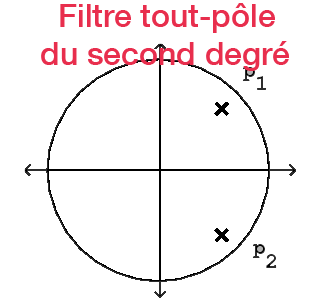
\includegraphics[scale=0.42]{Images/filtre}
					\end{figure}\noindent
				\end{minipage}
		\subsubsection{Autre}
			%\paragraph{\green{Bon outil pour traitement basique de signal}} WAVESURFER.
			\paragraph{\green{Description haut niveau d'un formant}}~\\
				\begin{minipage}{0.5\textwidth}
					\begin{figure}[H]
						\centering
						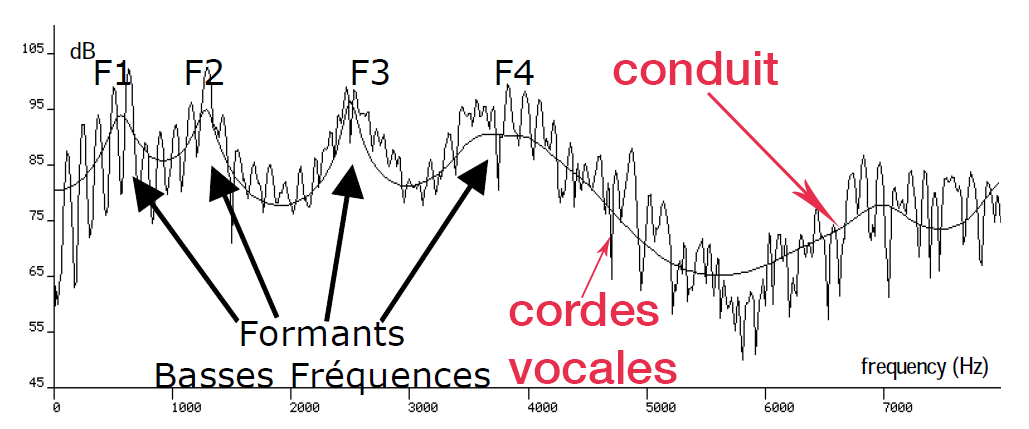
\includegraphics[scale=0.33]{Images/formant}
					\end{figure}\noindent
				\end{minipage}\hfill
				\begin{minipage}{0.45\textwidth}
					On peut donc en dire que la partie conduit vocal ne change pas si on ne change pas de lettre.
					Un "a" aigu aura les même formants qu'un "a" grave. Ce qui change entre un "a" aigu et un "a"
					grave c'est le rapprochement des sinusoïdes formées par les cordes vocales (=> fréquence
					produite par conduit vocal).
				\end{minipage}
	\pagebreak		
	\subsection{An Introductory Course on Speech Processing}
		\paragraph{\red{Dissocier le traitement de la parole du traitement du signal}}~\\~\\
			\point Les \hl{signaux telecom} (étudiés par le traitement du signal)
			sont les signaux les plus simples; 
			\alinea ils sont \hl{cr\'e\'es par des machines}
			d'ingénieur et sont reçus par des machines construites \\\alinea par des ingénieurs également.\\
			\point La \hl{parole est un signal cr\'e\'e par un cerveau} et ce signal
			est fait pour être compris par un \\\alinea cerveau
			également. \hl{Les signaux biologiques \'etaient l\`a bien avant les ing\'enieurs}, 
			donc plutôt \\\alinea que de
			le créer/modifier, on va essayer de le comprendre.
		\paragraph{\red{Justifier par une raison valable la complexité du signal de parole}}~\\~\\
			\point Le cerveau humain est plus complexe que n'importe quelle machine crée par l'homme,
			\\\alinea et la complexité d'un signal est fonction de la complexit\'{e}\ de\ l'\'{e}metteur\ 
			et\ de la complexité \\\alinea du\ receveur
		\paragraph{\red{Citer les principales sciences et techniques concernées par le traitement de la parole}}
			\begin{itemize}
				\setlength{\itemsep}{0pt}
				\setlength{\parskip}{0pt}
				\setlength{\parsep}{0pt}
				\item \myul{Informatique} : Les outils utilisés pour traiter la parole.
				\item \myul{Mathématique} : Mathématisation très forte de la parole.
				\item \myul{Linguistique et linguistique informatique} : Le signal reçu fait parti d'une langue.
				\item \myul{Ingénierie} : Il faut construire des machines capable de comprendre/traiter ce signal.
			\end{itemize}
		\paragraph{\red{Identifier les domaines de recherche du traitement de la parole}}
			\begin{itemize}
				\setlength{\itemsep}{0pt}		
				\setlength{\parskip}{0pt}		
				\setlength{\parsep}{0pt}
				\item \myul{Alphabet phonétique international} : On travail toujours sur la précision de cet alphabet.
				\item \myul{Codage de la parole} : Comment encoder un signal de voix sur l'ordinateur?
				\item \myul{Synthèse vocale} : Créer de la voix par ordinateur.
				\item \myul{Reconnaissance vocale} : Comprendre la voix humaine sur ordinateur.
			\end{itemize}
\pagebreak
	\subsection{Acoustics}
		\myul{Acoustique}: comprendre la \hl{physique derri\`ere le signal} de la parole
		%
		\paragraph{\red{Nommer les 7 profils de spécialistes travaillant en traitement de la parole.}}
			\begin{itemize}
				\setlength{\itemsep}{0pt}		
				\setlength{\parskip}{0pt}		
				\setlength{\parsep}{0pt}
				\item \myul{Indépendant de la langue} :
					\begin{itemize}
				 		\setlength{\itemsep}{0pt}		
				 		\setlength{\parskip}{0pt}		
				 		\setlength{\parsep}{0pt}	
				 		\item Acousticiens
						\item Phonéticien
				 	\end{itemize} 	
				 \item \myul{Dépendant de la langue} :
					\begin{itemize}
				 		\setlength{\itemsep}{0pt}		
				 		\setlength{\parskip}{0pt}		
				 		\setlength{\parsep}{0pt}	
				 		\item Phonologie
						\item Morphologie
						\item Syntaxe
						\item Sémantique
						\item Pragmatique
				 	\end{itemize}
			\end{itemize}
		\paragraph{\red{Expliquer en quoi consiste le travail d'analyse d'un acousticien.}}~\\~\\
			\point Leur travail consiste à analyser un signal acoustique, et donc, ils en analysent : 
			\begin{itemize}
				\setlength{\itemsep}{0pt}		
				\setlength{\parskip}{0pt}		
				\setlength{\parsep}{0pt}	
				\item La fréquence fondamentale du signal.
				\item L'amplitude du signal.
				\item Le spectre de fréquence du signal.
			\end{itemize}
		
		\paragraph{\red{Définir ce qu'est un audiogramme, comment on l'obtient et préciser quels traits 
		acoustiques \hspace*{0.035cm} il permet de mettre en évidence}}~\\ ~\\
			\point Courbe qui représente en fonction du temps l'intensité du son en fonction du temps et il
			\\\alinea permet de calculer les valeurs citées précédemment (la fréquence fondamentale du signal,
		    \\\alinea l'amplitude du signal, le spectre de fréquence du signal). 
			\\\alinea On y représente donc la \hl{variation de la pression par rapport \`a la pression acoustique}.
			\\
			\point Il permet de mettre en évidence les variations de pression causés par le conduit vocal.	
			\\\alinea On peut noter que sans l'aide des phonèmes (les sons produits par le conduit vocal),  
			\\\alinea aucun oeil humain ne peut déchiffrer tel quel un audiogramme.
			
		
		\paragraph{\red{Différencier sur un audiogramme les signaux voisés des signaux non voisés}}~\\~\\
			\point \myul{Signaux voisés} : Signal à structure périodique faisant intervenir les cordes vocales.\\
			\point \myul{Signaux non-voisés} : Signal ne faisant pas intervenir les cordes vocales.\\~\\
			%
			\begin{minipage}{0.55\textwidth}
				\alinea On peut donc les distinguer sur un audiogramme car les \hl{signaux vois\'es} montrent une 
				structure
			\hl{plus ou moins p\'eriodique}. \\\alinea En tout cas, on a l'impression qu'il est périodique mais en 
			réalité, 
			les nombres
			représentant le signal ne permettent pas de retrouver une période à ce signal, c'est notre cerveau
			et son intelligence qui permet d'imaginer une périodicité (d'environ 10 ms) à ce signal.
			\end{minipage}\hfill
			\begin{minipage}{0.4\textwidth}
				\begin{figure}[H]
					\centering
					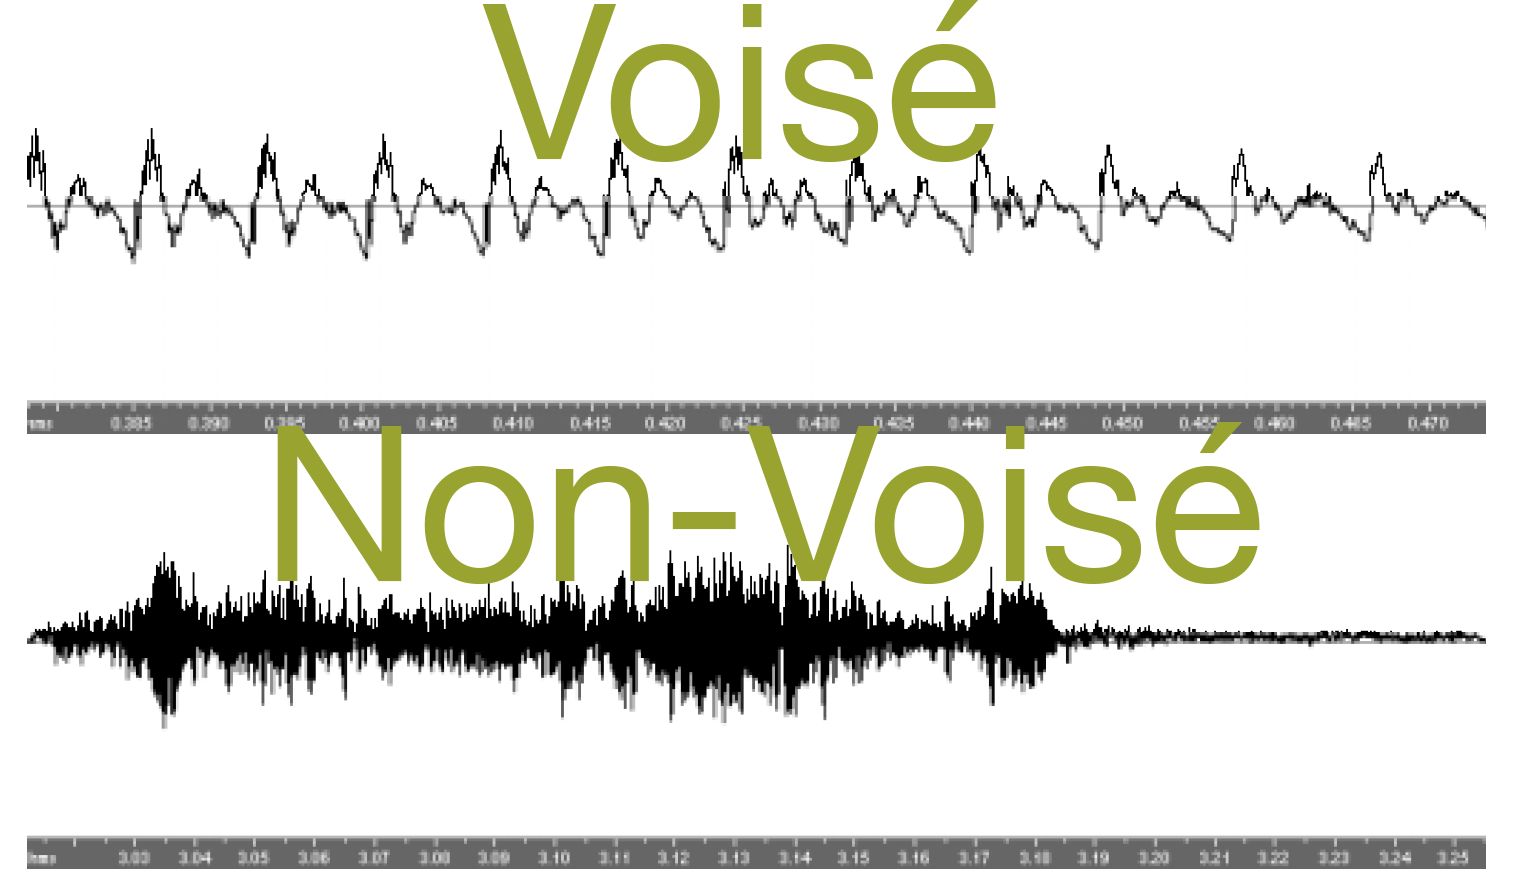
\includegraphics[scale=0.25]{Images/voise}
				\end{figure}
			\end{minipage}		
		\paragraph{\red{Décrire le résultat d'une analyse de Fourier et préciser quels traits acoustiques elle 
		permet \hspace*{0.035cm} de mettre en évidence}}~\\~\\
			\point \myul{L'analyse de Fourier} prend en entrée un signal (30ms en pratique) et donne en sortie
			les \\\alinea signaux formants du signal.\\
			%
			\point Une analyse de Fourier sur un signal voisé met en évidence la fréquence fondamentale et ses
			\\\alinea harmoniques (se trouvant à des fréquences multiples de la fondamentale) et ce \hl{pour 
			chaque}\\\alinea \hl{formant du signal}.\\
			%
			\point Une analyse de Fourier sur un signal non-voisé ne montre pas de fréquence fondamentale,
			\\\alinea (et donc pas d'harmoniques) mais seulement des pics d'amplitude qui sont les formants.
		
		\paragraph{\red{Caractériser ce qu'est un formant}}~\\~\\
			\point \myul{Formant} : Résonance de l'enveloppe spectrale du signal vocal. Il(s) change(nt)
				\\\alinea lorsque le conduit vocal change de forme.\\
			\point Lorsqu'on garde la même voyelle, le conduit vocal \hl{ne change pas de forme}, 
				\\\alinea et l'enveloppe spectrale reste donc identique : les formants ne bougent pas.\\
			\point La position des formants indiquent le son prononcé.
			
		\paragraph{\red{Différencier formant et fondamental}}~\\~\\
			\point \myul{Fondamentale} : La fondamentale est un signal qui se répète en harmonique.
				\\\alinea Lorsque l'on change la note sur une même voyelle, les formants ne bougent pas mais
				\\\alinea la fondamentale et ses harmoniques oui.\\
			\point \myul{Formant} : Un formant étant une fréquence de résonance de l'enveloppe spectrale d'un
				\\\alinea son, un signal sinusoïdal ou quasi-sinusoïdal ne définit pas de formant.
		\pagebreak
		\paragraph{\red{Décrire le principe de construction d'un spectrogramme, préciser son utilité et son 		
		~\\ \hspace*{0.035cm} utilisation}}~\\~\\
			\point \myul{Un spectrogramme} permet de combiner les informations de l'analyse de Fourier et
			de \\\alinea l'audiogramme. Il consiste en des analyses spectrales par fenêtres de temps.\\
			\point Il est constitué de \hl{3 dimensions}. On reprend la \hl{fr\'equence}, il devient l'axe vertical,
			\\\alinea l'axe horizontal étant le \hl{temps} (qui n'était pas présent dans une analyse spectrale, 
			étant  \\\alinea donné qu'on se concentrait sur une petite portion de temps). La troisième dimension
			est le \\\alinea niveau de gris représentant l'\hl{amplitude} du signal.\\
			\point On multiplie le signal par des fenêtres de temps qui se recouvrent un peu (pas forcément
				\\\alinea des fenêtres linéaire, souvent des courbes genre Gaussienne aplatie).	
			\begin{figure}[H]
				\centering
				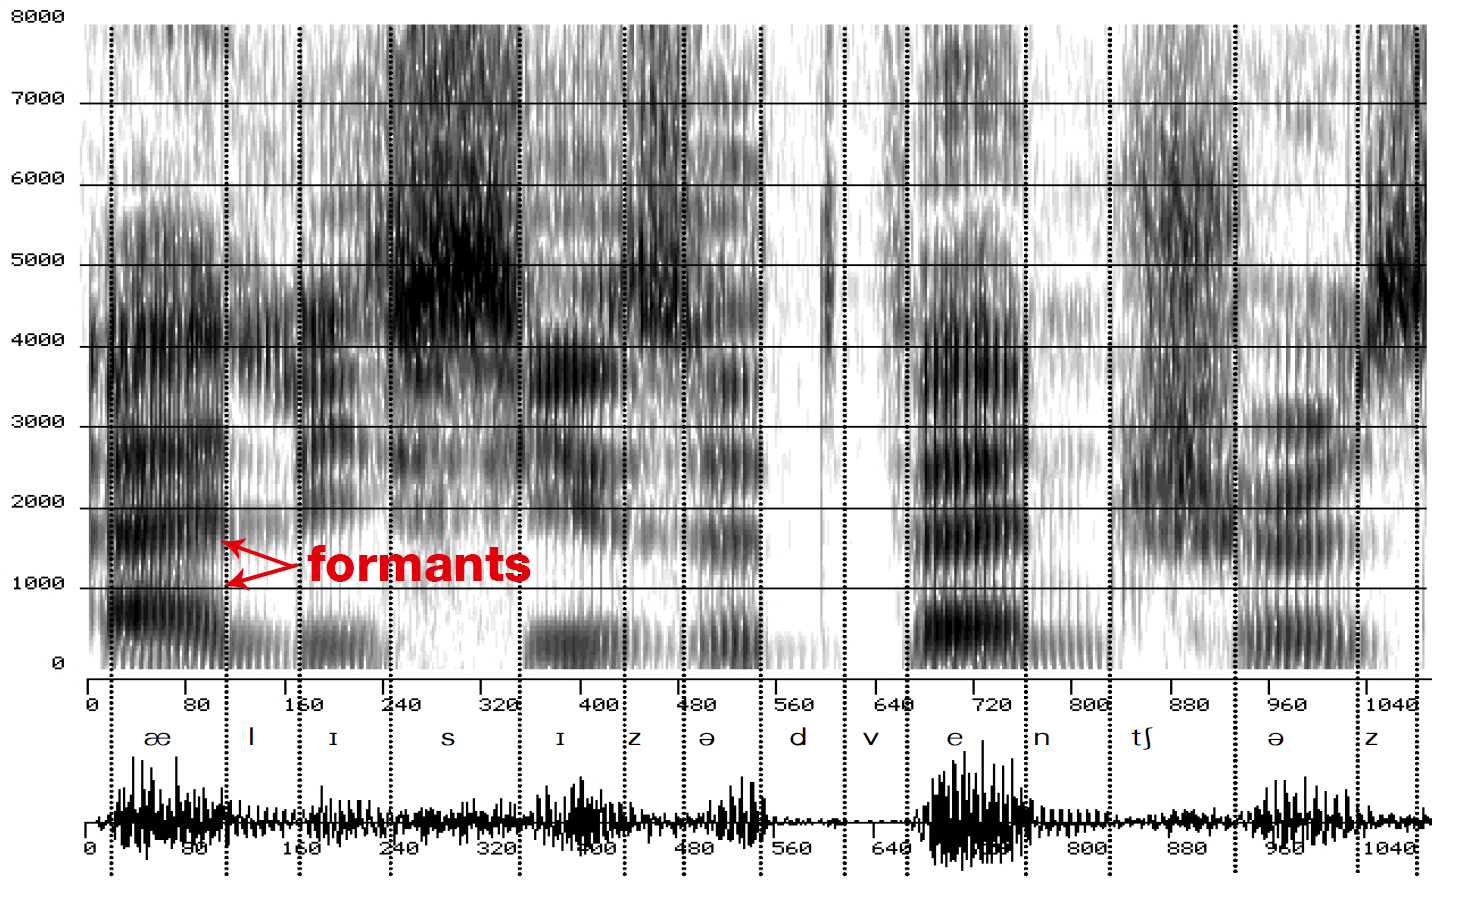
\includegraphics[scale=0.33]{Images/spectrogram}
			\end{figure}\noindent
			\point Le spectrogramme est le premier outil qui permet une analyse à l'oeil nu. Avec beaucoup 	
			\\\alinea d'expérience on pourrait en déduire directement les sons émis. On ne peut par contre 
			\\\alinea toujours pas connaitre l'intonation avec laquelle les sons ont été émis.
			
		\paragraph{\red{Dessiner une courbe typique d'intonation et en expliquer l'utilité}}~\\~\\
			\point \myul{Courbe de pitch} : Courbe représentant le déplacement de la fondamentale en fréquence
				\\\alinea des cordes vocales du conduit vocal. Cette courbe permet de regrouper les paquets de
				\\\alinea sons qui vont ensemble. Sans cette variation de fréquence, on aurait du mal à 
				savoir \\\alinea quand un mot se finit et que le prochain commence.
			\begin{figure}[H]
				\centering
				"les techniques de traitement numériques de la parole"
				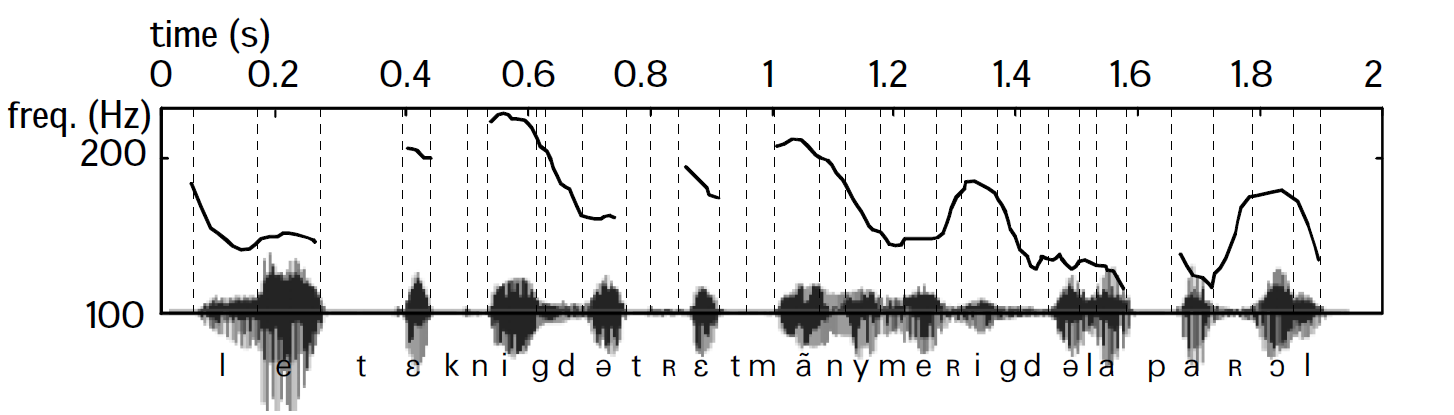
\includegraphics[scale=0.3]{Images/pitch}
			\end{figure}\noindent

\pagebreak

	\subsection{Phonectics}
		\myul{Phonétique}: \hl{diff\'erencier les sons} présents dans les langues 		
		%
		\paragraph{\red{Donner un diagramme schématique du conduit vocal et des cordes vocales et en décrire le 
			\hspace*{0.035cm} fonctionnement.}}~\\
			\begin{figure}[H]
				\centering
				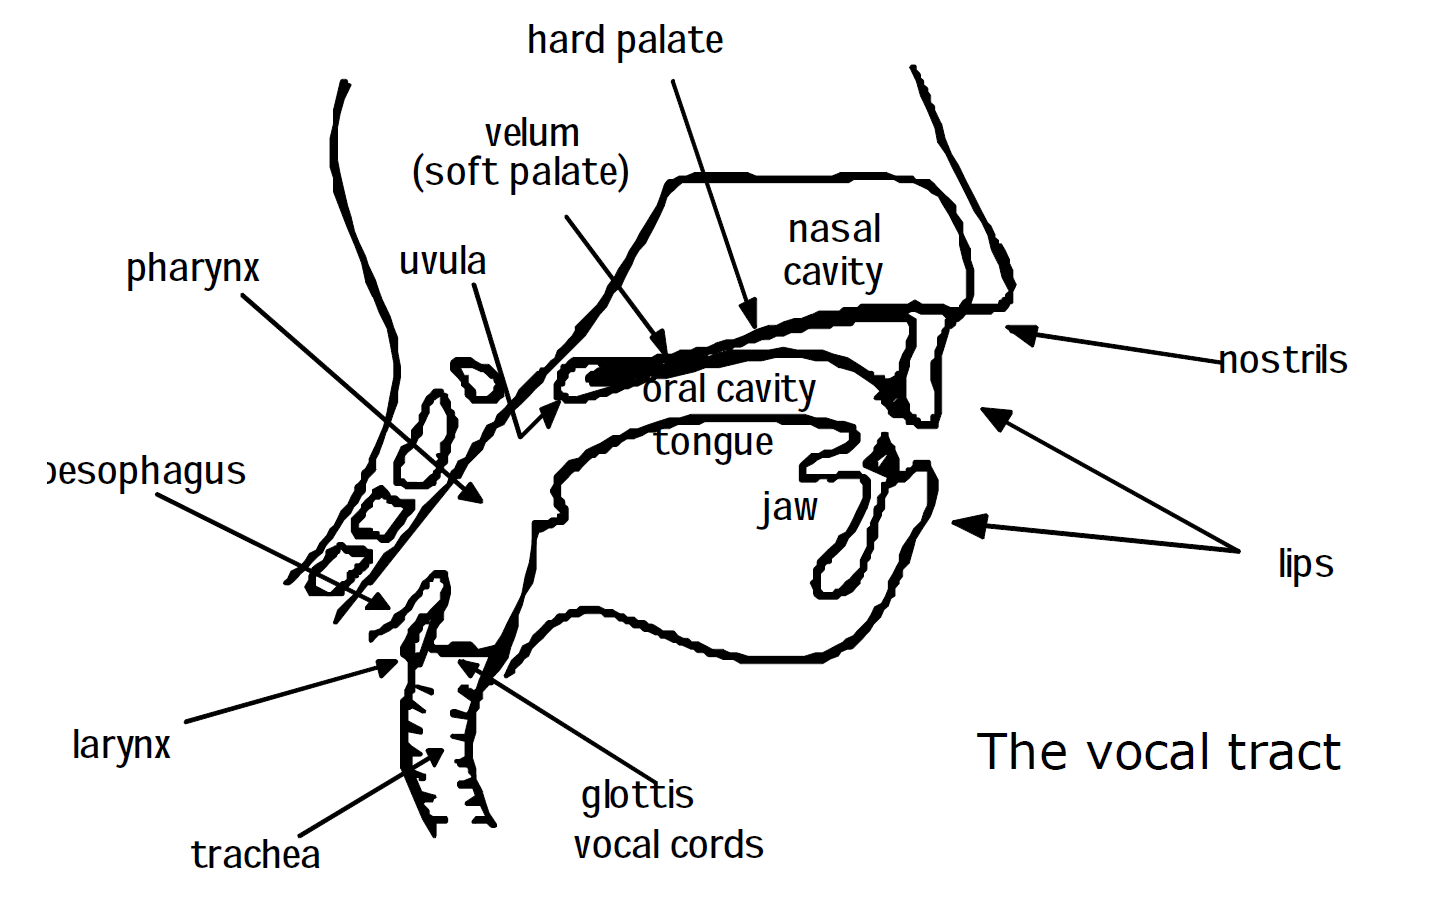
\includegraphics[scale=0.45]{Images/vocal_cavity}
			\end{figure}\noindent
			\begin{minipage}{0.4\textwidth}
				\begin{figure}[H]
					\centering
					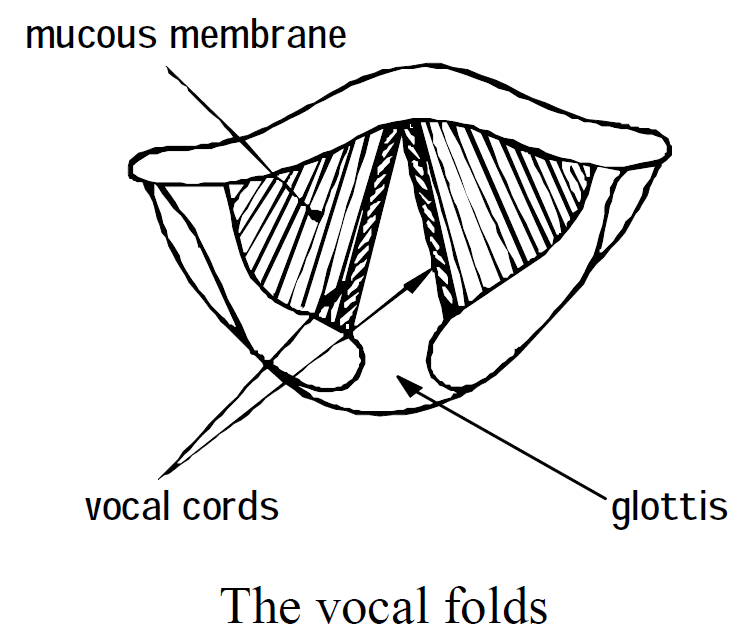
\includegraphics[scale=0.45]{Images/vocal_cords}
				\end{figure}\noindent
			\end{minipage}\hfill
			\begin{minipage}{0.4\textwidth}
				\begin{enumerate}
					\setlength{\itemsep}{0pt}		
					\setlength{\parskip}{0pt}		
					\setlength{\parsep}{0pt}	
					\item \hl{Membranes tendues} par les muscles qui tendent les cartilages autours d'elles.  
					\item Comme les cordes vocales sont fermées, la \hl{pression augmente} du à l'afflux d'air
						des poumons.
					\item \hl{Ouverture} due à la pression.
					\item Perte de pression => \hl{son brut \'emis} (modifié par la mâchoire, le larynx, ...) .
					\item \hl{Fermeture} et retour à l'étape 2. (=> périodique)
				\end{enumerate}
			\end{minipage}
			\begin{figure}[H]
				\centering
				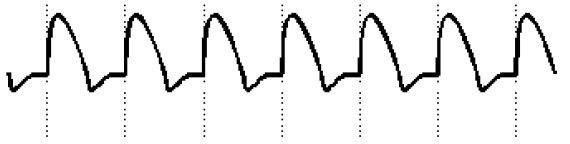
\includegraphics[scale=0.5]{Images/vocal_cords2}
			\end{figure}\noindent
			Plus les muscles sont tendus, plus la fréquence sera faible, et donc plus la période sera grande.
		
		\paragraph{\red{Citer et détailler les principaux modes de classification articulatoires en soulignant leurs 
		\hspace*{0.035cm} différences de principes.}}
			\begin{itemize}
				\setlength{\itemsep}{0pt}		
				\setlength{\parskip}{0pt}		
				\setlength{\parsep}{0pt}	
				\item \myul{Mode voyelle} : L'air passe \hl{sans encombre}, sans obstacle particulier.
					\begin{itemize}
						\setlength{\itemsep}{0pt}		
						\setlength{\parskip}{0pt}		
						\setlength{\parsep}{0pt}	
						\item Mode voyelle nasale : utilise les cavités nasales.
						\item Mode voyelle orale : utilise la cavité orale uniquement.
					\end{itemize}
				\item \myul{Mode consonne} : L'air passe par une \hl{constriction} (obstruction respiratoire
					en un point d'articulation donné) dans le canal vocal.
					\begin{itemize}
						\setlength{\itemsep}{0pt}		
						\setlength{\parskip}{0pt}		
						\setlength{\parsep}{0pt}	
						\item Mode consonne nasale : Obstruction totale.
						\item Mode consonne fricative : Blocage partiel quelque part. $<fff>\ <sss>$
						\item Mode consonne plosives : Son tenu suivi d'un blocage total suivi d'une "explosion"
							 $<parenTH\grave{e}se>$
						\item Mode consonne liquide : Sons caractérisés par une vibration basse fréquence, soit des 
							lèvres soit de la glotte.
					\end{itemize}
				\item \myul{Mode semi-voyelle} : \hl{Pas d'obstacle important mais pas tenu} $<ye>\ <we>$
			\end{itemize}
		% QUESTION : Est-ce qu'on doit retenir les sous-modes ?
		\paragraph{\red{Présenter par un exemple la classification par lieux d'articulation}}~\\~\\
			\point On peut parler de voyelle avant, arrière ou centrale. (passage\ de\ $\acute{e}\ \rightarrow\ o$).
			\\\alinea On change de lieu selon l'espace qu'on laisse au son pour qu'il se développe.\\
			\point On peut changer le lieu d'obstruction des consonnes (h aspiré + bouger sa glotte...)
		
		\paragraph{\red{Donner un exemple des caractéristiques complémentaires de sons exploitées en phonétique}}
			\begin{itemize}
				\setlength{\itemsep}{0pt}		
				\setlength{\parskip}{0pt}		
				\setlength{\parsep}{0pt}	
				\item \myul{Ouverture des voyelles} : $ \acute{e} $ = fermé, $ \grave{e} $  = ouvert.
				\item \myul{Voyelles tendues/breathée} = $a$ motivé / $a$ pas motivé
				\item \myul{Plosives apirées/non aspirées} = $pfff$ ou $p$
			\end{itemize}
		
		
		\paragraph{\red{Expliquer le principe qui a conduit à l'élaboration de l'alphabet phonétique international}}
		~\\~\\
			\point Chaque son peut être caractérisé par une suite binaire de caractéristiques phonétiques.
			\\\alinea (Ex: oral = 1, nasal = 0, ou encore labial = 1, non-labial = 0, ...).
			\\\alinea \hl{Chaque suite binaire donne une lettre de l'alphabet phon\'etique}.
		
		
		\paragraph{\red{Établir le lien entre la description acoustique et phonétique de la parole}}~\\~\\
			\point \myul{Description acoustique} : Analyse en fréquence, en formants.\\
			\point \myul{Description phonétique} : Analyse en lettre de l'alphabet phonétique.\\~\\
			%
			\begin{minipage}{0.4\textwidth}
			\begin{figure}[H]
				\centering
				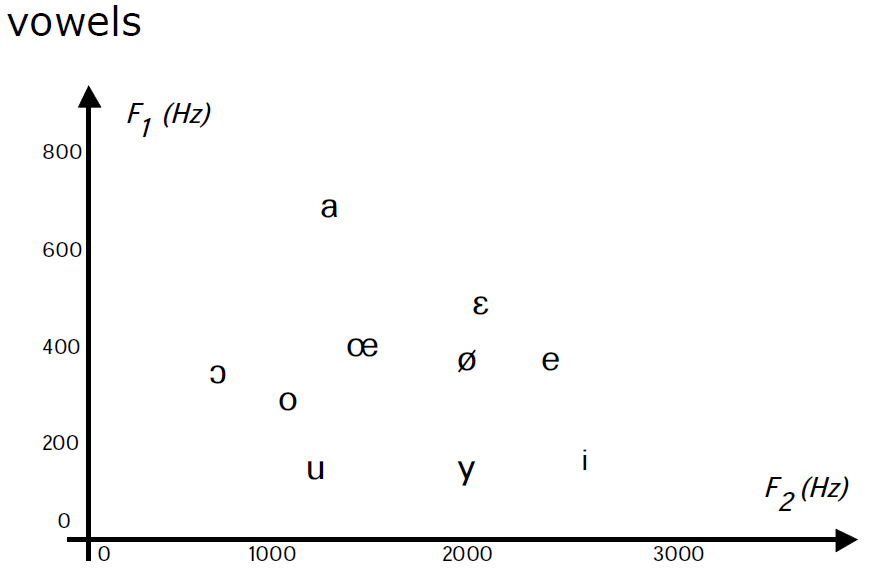
\includegraphics[scale=0.4]{Images/phonetic-acoustic}
			\end{figure}\noindent
			\end{minipage}\hfill
			\begin{minipage}{0.55\textwidth}
				On peut remarquer qu'on peut déterminer la voyelle à laquelle nous avons affaire simplement
				en mettant en graphique la relation entre les fréquences des deux premiers formants.
			    (On aurait pu établir une troisième dimension pour le troisième formant).\\~\\
			    En fait, les cordes vocales, pour produire une voyelle, se configure dans une forme particulière,
			    Ce qui donne des fréquences de résonance: les formants des acousticiens.\\
			    \hl{On en d\'eduit donc que les phon\'eticiens ont donn\'e une description phon\'etique du signal 
			    de parole.}
			\end{minipage}
		
		
		\paragraph{\red{Définir ce que l'on entend par « niveau de description segmental », par opposition au niveau
		\hspace*{0.035cm} « suprasegmental »}}~\\~\\
			\point \myul{Description Segmental} : description en fonction du \hl{mode} et du 
				\hl{lieu d'articulation}.		
			\point \myul{Description Suprasegmentale} : description de l'intonation.
		\paragraph{\red{Citer les trois caractéristiques globalisées par le terme « prosodie »}}~\\~\\
			\point \myul{Description Suprasegmental (prosody)} : Description en fonction du \hl{pitch}, \hl{dur\'ee} 
			et \\\alinea \hl{intensit\'e} du son. Il n'y a pas d'accord des phonéticiens à ce niveau.
		
	\subsection{Phonology}
		\myul{Phonologie}:\hl{ diff\'erencier les sons entendus et ce qu'on a voulu dire}.	
		%	
		\paragraph{\red{Différencier les niveaux de description de la parole dépendant de la langue des niveaux qui 
			~\\ \hspace*{0.035cm} n'en dépendent pas.}}~\\~\\
			\point Acoustique et Phonétique sont indépendants de la langue, tandis que la Phonologie, 
			\\\alinea la Morphologie, la Syntaxe, la Sémantique et les Pragmatiques en sont dépendants.\\
			\point On passe d'une \hl{analyse objective} de la parole (niveaux indépendant de la langue) à une 
			\\\alinea \hl{analyse presque subjective} de la langue (niveaux dépendants de la langue).
		
		\paragraph{\red{Donner la définition de phonème et le nombre de phonèmes dans la langue française.}}~\\~\\
			\point \myul{Phon\`eme} : \hl{Son abstrait} dans le cerveau de la personne qui parle, et 
				\\\alinea \hl{chaque son s'oppose \`a tous les autres}, non pas par ce qui est dit, mais par
				\\\alinea \hl{leur intention}. Ils représentent donc les sons que le cerveau imagine avant
				\\\alinea de les envoyer au canal vocal. Il y a \hl{36 phon\`emes} dans la langue française.
		
		\paragraph{\red{Donner un exemple d'allophone.}}~\\~\\
			\point \myul{Allophone} : \hl{Plusieurs sons} à la phonétique différente (e.g. $R$ normal ou $R$ roulé)
				\\\alinea \hl{pour un m\^eme phon\`eme}.
			\begin{itemize}
				\setlength{\itemsep}{0pt}		
				\setlength{\parskip}{0pt}		
				\setlength{\parsep}{0pt}	
				\item Les variantes géographiques : Si un auvergnat roule ses $R$, ce n'est pas voulu,
					ça ne change pas le sens du mot pour autant.
				\item La coarticulation : On est constamment en train de gérer un transitoire dans les cordes
					vocales pour faire sortir un son voulu, mais qui ne sera jamais le bon en réalité
					(car son trop compliqué ou contraintes physiques). Exemple: entre ann$ue$l et act$ue$l,
					notre cerveau voudrait faire sortir le même phonème pour les deux mots, mais il en sort
					deux sons phonétiquement différents, on "siffle" le u de actuel, et pas celui de annuel.
					% QUESTION : c'est bien ca pour la coarticulation ?
			\end{itemize}
		
		\paragraph{\red{Citer et définir sur base d'un exemple (à donner) la principale distinction entre phonème et 
		~\\ \hspace*{0.035cm} son (ou phone).}}~\\~\\
			\point Un phon\`eme est définit par une \hl{intention de faire parvenir un son} par le canal vocal.\\
			\point Le son est défini par \hl{le son r\'eel} qui sort du canal vocal.\\
			\point La différence entre les deux s'explique par le principe de coarticulation. (e.g. ann$ue$l/act$ue$l)
		
		\paragraph{\red{Commenter l'affirmation suivante : « Lorsqu'on connaît le fossé qui sépare la  
		~\\ \hspace*{0.035cm} représentation acoustique de la parole de son niveau phonologique, la communication 
		~\\ \hspace*{0.035cm} parlée tient du miracle ».}}~\\~\\
			\point Le miracle c'est que malgré que le mauvais son sorte, celui qui écoute est persuadé que le
				\\\alinea bon son est sorti, il a donc compris le phon\`eme alors que le son n'y correspondait pas 
				\\\alinea forcément.
		
		\paragraph{\red{Justifier l'expression « C'est du chinois ! » du point de vue de la phonologie.}}~\\~\\
			\point Le chinois est une \hl{langue \`a ton}, c'est à dire que l'intonation a un sens dans la langue.
				\\\alinea chaque intonation désigne un mot différent, apporte un information particulière.\\
			\point Il est assez compliqué d'apprendre une langue à ton quand on en parle pas une car 
				\\\alinea depuis l'enfance, le cerveau a appris à ne pas faire de distinction de phon\`eme 
				\\\alinea entre deux intonations différentes.
				
		\pagebreak
		
		\paragraph{\red{Définir la coarticulation et en justifier son impact en traitement de la parole en 
		~\\ \hspace*{0.035cm} l'illustrant par un schéma.}}~\\
			\begin{minipage}{0.55\textwidth}
				\point La coarticulation : Ph\'enom\`ene qui est du au fait \\\alinea que le 
				\hl{conduit vocal est un syst\`eme
				physique} qui \\\alinea poss\`ede une \hl{inertie} qui lui est propre, 
				\\\alinea et donc, il est \hl{impossible} à 
				 un \^etre humain de \\\alinea \hl{passer infiniment rapidement d'un son \`a un autre}.\\
			\point La coarticulation implique que \hl{chaque son \'emis} \\\alinea \hl{est diff\'erent}, même s'il 
				est sensé désigner un même \\\alinea phon\`eme.
			\end{minipage}\hfill
			\begin{minipage}{0.4\textwidth}
				\begin{figure}[H]
					\centering
					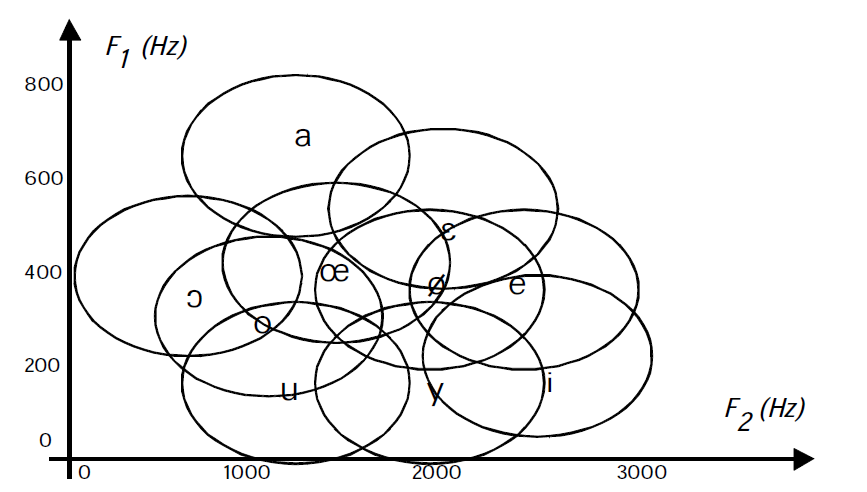
\includegraphics[scale=0.5]{Images/coarticulation}
				\end{figure}\noindent
			\end{minipage}
			\point La \hl{synth\`ese vocale} est affect\'ee par la coarticulation parce qu'il faut \^etre capable 
				\\\alinea de l'\hl{imiter}. En effet, si on ne respecte pas la coarticulation, les gens ont
				\\\alinea beaucoup de mal à comprendre ce qui est dit.\\
			\point La \hl{reconnaissance vocal} est affect\'ee par la coarticulation parce qu'il faut pouvoir 
				\\\alinea la surmonter, et savoir \hl{quel phon\`eme \'etait voulu} par rapport au son émis. 
	
	\subsection{Morphology}
		\myul{Morphologie}: \'etude de l'assemblage de sons pour faire un mot.
		%
		\paragraph{\red{Donner un ordre de grandeur du nombre de mots d'une langue naturelle (comme la langue 
		~\\ \hspace*{0.035cm} française) et du nombre de mots utilisé dans le langage quotidien}}~\\~\\
			\point L'ordre de grandeur est de 50 000 mots dans le dictionnaire, et en y ajoutant les noms
				\\\alinea masculin/féminin/pluriels, on tombe sur 500 000 voir 1 000 000 de mots.\\
			\point On utilise dans le langage quotidien environ 5000 mots.	
		
		\paragraph{\red{Définir ce qu'est un morphème et en donner un exemple}}~\\~\\
			\point \myul{Morpheme} : \hl{Unit\'e abstraite} qui compose les mots et qui apporte, chacune, une 
				\\\alinea \hl{information de sens}. \\
			\point Ces unités sont programmées dans le cerveau, encodées sous forme de mots qui respectent 
				\\\alinea un certain nombre de règles (règles de morphologie de la langue). ~\\
				\\\alinea Exemple : went = $go$ + $past$, visible = $see$ + $able$. ~\\~\\
		
		\paragraph{\red{Citer et expliquer les trois procédés (règles) morphologiques fondamentaux d'une 
		~\\ \hspace*{0.035cm} langue naturelle}}
			\begin{itemize}
				\setlength{\itemsep}{0pt}		
				\setlength{\parskip}{0pt}		
				\setlength{\parsep}{0pt}	
				\item Flexion : Entrée : un morphème lexicale + un morphème grammatical et donne un nouveau mot 
					qui a la \hl{m\^eme nature que le morph\`eme lexical de d\'epart}. 
					(conjugaison des verbe, passage au pluriel, ...)
				\item Dérivation : Entrée : morphème lexical + morphème grammatical et donne un nouveau mot
					qui n'a \hl{pas la m\^eme nature que le morph\`eme lexical de d\'epart} 
					(image $\rightarrow$ imaginer, imagination, ...).
				\item Composition morphologique : Entrée : plusieurs morphèmes lexicaux et les \hl{composer} en
					un nouveau mot (rouge-gorge, sous-marin, ...).
			\end{itemize}
				
		\paragraph{\red{Illustrer par deux exemples le fait que chaque langue utilise à sa façon les trois procédés de 
		~\\ \hspace*{0.035cm} transformation morphologique}}~\\~\\
			\point La flexion des verbes en français fait apparaitre 41 formes verbales, alors qu'en anglais on  
			\\\alinea en trouve que 8. Donc la façon dont on utilise la morphologie de la langue dépend de la 
			\\\alinea \hl{complexit\'e} de formation des mots de la langue.
		
	\subsection{Syntax}
		\myul{Syntaxe}: \'etude de l'\hl{ordre} dans lequel les \hl{mots} peuvent se retrouver 
			(sujet -> verbe -> complément)
		%
		\paragraph{\red{Donner le but premier de l'analyse syntaxique}}~\\~\\
			\point Le but est de faire le tri parmi les suite de mots de la langue, les \hl{suites de mots possibles}
				\\\alinea et les suites de mots impossibles.
		
		\paragraph{\red{Distinguer syntaxe et grammaire}}~\\~\\
			\point \myul{Syntaxe} : \hl{Contraintes abstraites} de la validité d'une suite de mot.\\
			\point \myul{Grammaire} : \hl{Formalisation} de la syntaxe à travers une grammaire (type de mots, ...).
				\\\alinea Elles sont crées par des grammairiens, spécialistes de la langue. Chaque spécialiste
				\\\alinea a sa façon de voir les choses (grammaire historique vs grammaire d'apprentissage).
		
		\paragraph{\red{Nommer le type de grammaires compréhensibles par un ordinateur (en donner un exemple)  
		~\\ \hspace*{0.035cm} et la discipline scientifique qui en découle}}~\\~\\
			\point Les grammaires de langue que l'on apprend à l'école sont des grammaires spéciales : 
				\\\alinea elles ont pour but de formaliser une langue qui est déj\`a parlée par l'étudiant.\\
			\point Les grammaires utilisables par l'ordinateur sont donc des grammaires qui ne \hl{supposent}
				\\\alinea \hl{aucune connaissance pr\'ealable de la langue}. Il faut donc lui donner des listes 
				\\\alinea de mots que le langage va utiliser. 
				\\\alinea Ex : les grammaires syntagmatiques (phrase = group\_nom + verb\_conj, 
					group\_nom = ...).\\
			\point \c Ca a donné naissance à la \hl{linguistique informatique} dans les années 50.
		
		\paragraph{\red{Justifier pourquoi il est intéressant de réaliser une analyse syntaxique, au delà de la 
		~\\ \hspace*{0.035cm} vérification de la validité syntaxique de la phrase}}~\\~\\
			\point \c Ca permet de former des \hl{groupes} de mots (groupe nominal, groupe sujet, ...) et ça va 
				\\\alinea beaucoup aider la synthèse et la reconnaissance vocale. La \hl{structuration} 
				\\\alinea syntaxique va donc permettre d'avoir une information sur le sens de la phrase
				\\\alinea (Exemple: [Time] [flies] [like an arrow] ou [Time flies] [like] [an arrow]).
	
	\subsection{Semantics \& Pragmatics}
		\myul{Sémantique}: \'etude liée à l'ordre des mots avec leur sens (lier l'objet qui se cache derri\`ere
			le mot avec d'autres mots). Exemple: un concept abstrait n'a pas de couleur (la richesse jaune ?).\\
		\myul{Pragmatique}: \'etude des sens caché dans les phrases (concepts n'ayant pas besoin d'être précisés
			pour être compris par un autre humain).
		%
		\paragraph{\red{Opposer syntaxe et sémantique}}~\\~\\
			\point \myul{Sémantique} : Faire le tri entre les suites de mots syntaxiquement correctes qui 
				\\\alinea \hl{veulent dire quelque chose} et celles qui ne veulent rien dire.
				\\\alinea Cependant, comme la syntaxe, c'est une idée abstraites qu'il faudra formaliser en grammaire.
		
		\paragraph{\red{Spécifier la base de construction des règles sémantiques}}~\\~\\
			\point La base des règles sémantiques sont les \myul{traits sémantiques}. Chaque mot a un
				\\\alinea ensemble de traits sémantiques et dans les règles de ces grammaires sémantiques, il
				\\\alinea y a des \hl{implication dans la concordance entre les traits s\'emantiques des mots}
				\hl{successifs.}
				\\\alinea Exemples de traits : mot abstrait, adjectif de couleur, ...\\
			\point On peut en conclure pas mal de choses. Ex : un mot abstrait ne peut pas être suivi d'un 
				\\\alinea adjectif de couleur (politesse jaune ?).\\
			%
			\point Un des problème qui se pose est : "comment définir un lexique informatique qui permet  
				\\\alinea de choisir un trait parmi les traits sémantiques". Une solution peut être de \hl{lister}
				\\\alinea \hl{de fa\c con exhaustive} tous les traits sémantiques liés à un vocabulaire 
				\\\alinea (ce qui n'est pas envisageable dans le cas de la langue entière).
		
		\paragraph{\red{Nommer et décrire par un exemple un problème classique de la sémantique. Désigner en  
		~\\ \hspace*{0.035cm} une phrase les caractéristiques de la parole concernées par la pragmatique}}~\\~\\
			\point \myul{\hl{Anaphore}} : Problème classique lié à des \hl{mots r\'ef\'erant \`a d'autres mots} 
				dans une phrase.
				\\\alinea \hl{Exemple} : "J'ai posé une tasse sur la table et puis je l'ai déplacée.". Rien
				\\\alinea ne permet de savoir de fa\c con formelle si on a déplacé la table ou la tasse.
				\\\alinea D'ailleurs, aucun système informatique ne peut le déterminer à ce jour.\\~\\
			%
			\point \myul{Pragmatique} : Concerne \hl{tout ce qui n'est pas trait\'e par les points pr\'ec\'edents}.
				\\\alinea On retrouve dedans tout ce qui, pour la bonne interprétation du message, nécessite
				\\\alinea des informations qui ne \hl{se trouve pas de mani\`ere textuelle dans la phrase} 
				(entre les lignes). \\\alinea Ou encore des phrases qui requièrent des informations concernant le
				monde dans lequel \\\alinea la phrase est dite.
				\\\alinea Exemple: Si on parle de disques placés l'un après l'autre sur une tige pour faire une
				\\\alinea serrure, ils ne vont pas être soudé parallèlement à la tige, mais rien ne le dit dans 
				le texte.
		
	\subsection{From Source To Receiver}
		
		\paragraph{\red{Décrire le fonctionnement de l'oreille et schématiser ses principales parties}}~\\
		\begin{figure}[H]
			\centering
			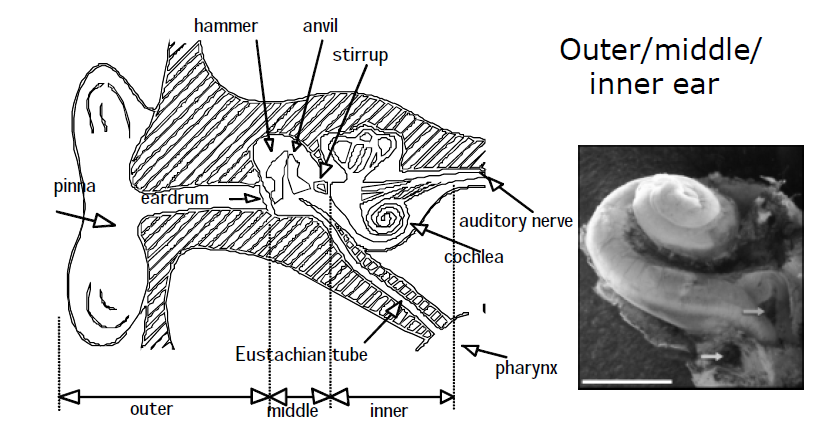
\includegraphics[scale=0.8]{Images/oreille}
		\end{figure}\noindent	
		\point L'oreille moyenne contient \hl{marteau, l'enclume et l'\'etrier}. L'oreille communique avec
			le nez \\\alinea par la trompe d'Eustache.\\
		\point L'\hl{\'etrier met en vibration} la fenêtre ovale qui est \hl{l'entr\'ee de la cochl\'ee} 
		(oreille interne)
		qui est un \\\alinea cone, enroulé sur lui même, rempli d'un liquide qui est mis en mouvement par le 
		mouvement \\\alinea  de l'étrier. \\
		\point Dans ce cone se trouvent des \hl{cellules cili\'ees} qui sont raccordées chacune
		a un nerf auditif. \\\alinea Le mouvement du liquide a l'intérieur du cône va créer des \hl{impulsions 
		\'electriques}
		qui vont \\\alinea être comprises par le cerveau.
		
		\paragraph{\red{Justifier l'analogie entre la cochlée et un analyseur spectral}}~\\~\\
			\point En fonction de la fr\'equence du signal qui est poussé par l'étrier, les zones
			du cône qui 
			\\\alinea sont mises en vibration varient. $\rightarrow$ ce ne sont pas les même cils qui seront 
			\\\alinea stimulés si on change de fréquence du son entendu.\\
			\point \hl{\`A chaque zone cili\'ee correspond une gamme de fr\'equence entendue}. 
			
\pagebreak
		
		\paragraph{\red{Justifier que la psychophysique ait permis de normaliser la transmission de parole sur les 
		~\\ \hspace*{0.035cm} canaux téléphoniques et traduire cette justification par un schéma}}~\\~\\
			\point \myul{Psychophysique} : Branche de la psychologie qui étudie le cerveau en faisant appel
				\\\alinea à des \hl{ressentis} de sujets de test. \\
			\begin{minipage}{0.4\textwidth}
				\begin{figure}[H]
					\centering
					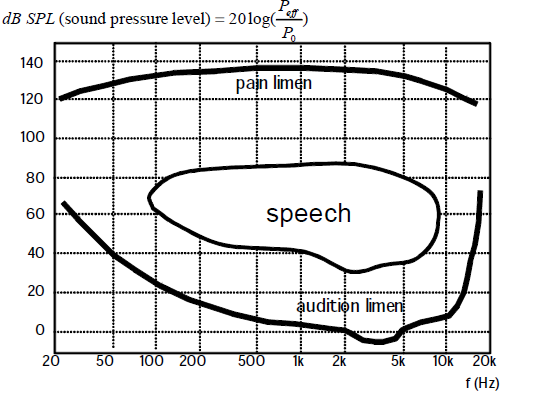
\includegraphics[scale=0.7]{Images/psychophysique}
				\end{figure}\noindent
			\end{minipage}\hfill
			\begin{minipage}{0.55\textwidth}
				\point En se basant sur le ressenti des gens, on a pu découvrir, en fonction de la fréquence, le
				\hl{seuil d'audition} et le \hl{seuil de douleur} de l'oreille humaine. \\
				\point En observant la courbe du seuil d'audition, on a pu \hl{formaliser} en 1929 \hl{les 
					fr\'equences}
					qui allaient être utilisée pour la \hl{t\'el\'ecommunication}: 300Hz $\rightarrow$ 3400Hz
			\end{minipage}
		
		\paragraph{\red{Donner la définition des courbes isosoniques et les comparer aux courbes de seuil de 
		~\\ \hspace*{0.035cm} l'audition et de seuil de la douleur}}~\\
			\begin{minipage}{0.4\textwidth}
				\begin{figure}[H]
					\centering
					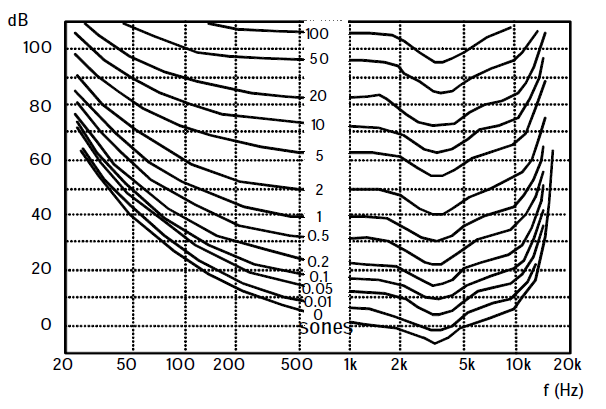
\includegraphics[scale=0.6]{Images/isosonic}
				\end{figure}\noindent
			\end{minipage}\hfill
			\begin{minipage}{0.55\textwidth}
				\point \myul{Courbes isosoniques} : courbes d'égales sensations acoustiques. Elles servent à 
					savoir quand est-ce qu'une fréquence peut être entendue avec la même intensité
					qu'une autre fréquence.\\
				\point Là ou le seuil d'audition et le seuil de douleur donnent des limites d'auditions,
					les courbes isosoniques donnent des informations sur \hl{l'\'equivalence d'intensit\'e}
					perçue pour deux fréquences différentes.
			\end{minipage}
			
\pagebreak

		\paragraph{\red{Décrire le phénomène de masquage auditif et donner un exemple d'impact technologique 
		~\\ \hspace*{0.035cm} en traitement de la parole}}~\\
			\begin{minipage}{0.4\textwidth}
				\begin{figure}[H]
					\centering
					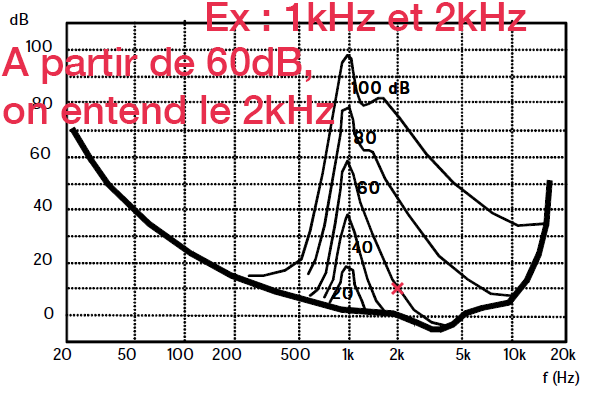
\includegraphics[scale=0.6]{Images/masquage}
				\end{figure}\noindent
			\end{minipage}\hfill
			\begin{minipage}{0.55\textwidth}
				\point \myul{Masquage auditif} : \hl{Fait qu'une fr\'equence peut ne pas \^etre entendue parce qu'elle
					est masqu\'ee par une autre fr\'equence}. Lorsque quelqu'un écoute une fréquence,
					il faut dépasser un \hl{nouveau seuil} pour que la nouvelle fréquence puisse être entendue.\\
				\point Ce masquage dépend à la fois de la fréquence, de l'amplitude du son de départ et de la
					\\\alinea fréquence du nouveau son à entendre. Ce phénomène peut devenir complexe car
					en réalité, il y a beaucoup de fréquences "masquantes" et de fréquences masquées.
			\end{minipage}
			%
			\point Dans les standardisation d'enregistrement sur média, on a décidé de ne stocker que les 
				informations qui seront perçues. Problème : on a des courbes moyennes, mais en réalité,
				certaines personnes peuvent entendre des distorsions que d'autres n'entendront pas.\\
			\point Lorsqu'on calcule des \hl{taux d'erreur}, il faut savoir que ces taux d'erreur n'auront pas
				toujours
				de signification forte, il faudra parfois les \hl{pond\'er\'es}. On les pondérera grâce à
				des \hl{mod\`eles de l'oreille} humaine (modèles perceptuels) afin de prendre en compte non
				pas la distorsion physique mais la distorsion perçue.\\
			\point On peut également dire qu'on va se limiter aux fréquences audible par l'humain et 
				ignorer les autres.
\pagebreak
\section{Modeling of the speech}

	\subsection{Autoregressive modeling of the speech}
		
		\paragraph{\red{Distinguer les deux étapes du processus de mise en œuvre d'un nouveau modèle de la 
		~\\ \hspace*{0.035cm} parole.}}
		\begin{itemize}
			\setlength{\itemsep}{0pt}		
			\setlength{\parskip}{0pt}		
			\setlength{\parsep}{0pt}	
			\item La \hl{cr\'eation du mod\`ele} en lui-même : établir quels paramètres feront parti du modèle.
			\item La mise au point d'\hl{algorithmes} qui permettent d'\hl{obtenir les param\`etres} de ce modèle : 
				on peut voir ca comme une boucle d'estimation, on essaie des paramètres, on compare le résultat avec
				le résultat souhaité, on change certains paramètres et on recommence. (On peut avoir plusieurs
				algorithmes d'estimation différents pour un même modèle)
		\end{itemize}
		
		\paragraph{\red{Différencier erreurs de modélisation et erreur d'estimation, et montrer que la création d'un 
		~\\ \hspace*{0.035cm} modèle résulte d'un compromis entre ces deux types d'erreurs.}}
		\begin{itemize}
			\setlength{\itemsep}{0pt}		
			\setlength{\parskip}{0pt}		
			\setlength{\parsep}{0pt}	
			\item \myul{Erreur de modélisation} : dû à un modèle trop simple qui conduit à une impossibilité d'obtenir 
				le résultat recherché.
			\item \myul{Erreur d'estimation} : si le modèle est trop compliqué, on peut avoir du mal à développer un 
				algorithme d'estimation.
		\end{itemize}
		Il faut donc trouver le \hl{juste \'equilibre entre mod\`ele pas trop compliqu\'e et pas trop simple}.

		\paragraph{\red{Citer et caractériser les trois grandes familles de modèles de la parole.}}
		\begin{itemize}
			\setlength{\itemsep}{0pt}		
			\setlength{\parskip}{0pt}		
			\setlength{\parsep}{0pt}	
			\item \myul{Modèle articulatoire} : les équations sont des équations de la 
				\hl{m\'ecanique des fluides}. On y représente par exemple les cordes vocales par un ensemble 
				de masses vibrantes. Les paramètres sont
				par exemple : la position de la langue, la forme du conduit vocal, ...
			\item \myul{Modèle de production} : modèle pour lesquels on symbolise la production de la parole à
				l'aide d'outils simples qui sont : des générateurs et des filtres. Ce modèle considère que la parole
				humaine est le résultat du passage d'un \hl{signal de base, simple \`a travers une s\'erie
				d'amplificateurs, de filtres}, ...
			\item \myul{Modèle phénoménologique} : modèle le plus mathématique, car \hl{se basent uniquement sur des 
				th\'eories de traitement de signal} pures (analyse de fourrier, ...)
		\end{itemize}
		
		\pagebreak
		
		\paragraph{\red{Présenter le modèle autorégressif de traitement de la parole en réalisant l'analogie avec le 
		~\\ \hspace*{0.035cm} syst\`eme naturel de production de la parole.}}~\\
			\vspace*{-1cm}
			\begin{figure}[H]
				\centering
				\includegraphics[scale=0.65]{Images/autoregressive}~\\
				Modèle autoregressif = modèle prédictif linéaire = LPC
			\end{figure}\noindent
			\begin{itemize}
				\setlength{\itemsep}{0pt}		
				\setlength{\parskip}{0pt}		
				\setlength{\parsep}{0pt}	
				\item \myul{Le signal glottique} va être modélisé par un \hl{signal num\'erique} 
					(suite d'impulsion de Dirac)
					passant par \hl{un filtre num\'erique \`a deux p\^oles r\'eels} : $\alpha$ et $\beta$. 
				\item On considère que \myul{le conduit vocal} joue le rôle d'une suite de résonateurs, suite 
					de système du second degrés à deux pôles. Ceci vient du fait qu'on considère donc que
					le conduit vocal produit des formants (résonances dans le spectre), et que donc on a besoin
					d'un nombre fini de systèmes résonants dont on va régler les coefficients $b_1$ et $b_2$
					et chaque paire de coefficient servira a régler un formant en terme de fréquence et d'amplitude.
				\item Le \myul{débit en pression} est réalisé par \hl{un simple syst\`eme num\'erique qui simule la
					d\'erivation}. 
					La pression est proportionnelle à la dérivée du débit. Cette opération de dérivation
					peut être simulée par l'équation $R(z)$ en traitement de signal. Le zéro de l'équation
					est en z = 1. La mise en cascade des 3 filtres va faire en sorte de camoufler le zéro 
					et ne faire apparaitre que les pôles.
			\end{itemize}
\pagebreak
		\paragraph{\red{Donner un schéma de principe du modèle LPC de traitement de la parole, citer ses paramètres 
		\hspace*{0.0325cm} et caractériser leur rôle.}}~\\
		\vspace*{-1cm}
		\begin{figure}[H]
			\centering
			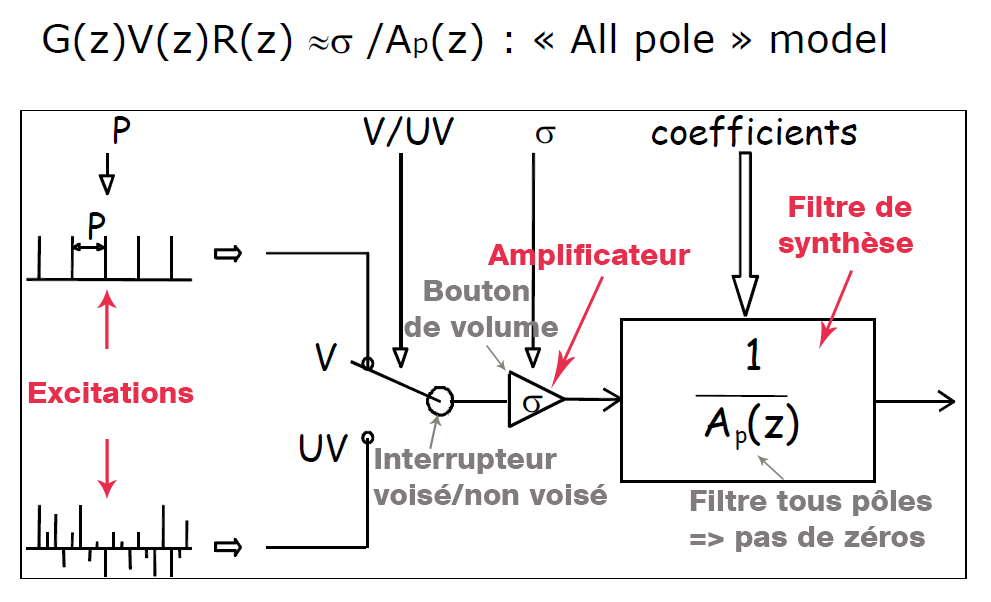
\includegraphics[scale=0.5]{Images/lpc}
		\end{figure}\noindent
		\alinea On considère que si le son est non voisé, il peut "tout de même" (même si on ne met pas en cascade 
			$G(z)$) être représenté par un filtre tous pôles.\\
		\alinea Les pôles du mod\`ele doivent rester dans le cercle unité pour que son filtre reste stable.
		
	\subsection{Autoregressive estimation of speech}
		
		\paragraph{\red{Expliquer pourquoi la modélisation autorégressive est basée sur un principe de  
		~\\ \hspace*{0.035cm} minimisation d'erreur.}}~\\~\\
			\point Le signal vocal n'est pas stationnaire. En effet, si le même son était entendu constamment, 
				\\\alinea on ne pourrait pas transmettre de l'information. Mais étant donné les contraintes physiques
				\\\alinea des cordes vocales, on peut considérer le signal vocal comme stationnaire sur 30ms.\\
			\point Chaque \hl{fen\^etre d'analyse} aura donc une largeur de \hl{30ms} et le 
				\hl{d\'ecalage entre chaque } 
				\\\alinea \hl{fen\^etre} est de \hl{10ms}. Ce qui permet de réduire l'erreur loors du 
				passage au numérique 
				\\\alinea sans pour autant demander trop de calculs.

		\paragraph{\red{Décrire le système d'équations de Yule-Walker, en expliquer les composantes et justifier sa 
		~\\ \hspace*{0.035cm} facilité de résolution.}}~\\~\\
			\point \myul{Système de Yule-Walker} : Système de p équations à p inconnues. La fonction $\phi_X$
				\\\alinea est appelée fonction d'auto-corrélation. On va la calculer sur 30ms depuis l'ordre 0 
				\\\alinea jusqu'à l'ordre p. \hl{Ces valeurs sont les potentiom\`etres du mod\`ele LPC}
				(coefficients).\\
			\point La matrice qui contient les valeurs de $\phi_X$ est une \hl{matrice de Toeplitz}(symétrie autour
				\\\alinea de la diagonale) ce qui permet de résoudre le système en \hl{$O(p^2)$} à la place de
				\\\alinea $O(p^3)$ pour un système standard (grâce à l'algorithme de Schur ou de Levinson).
			\begin{figure}[H]
				\centering
				\includegraphics[scale=0.5]{Images/Yule}
			\end{figure}\noindent
		
		\paragraph{\red{Préciser l'avantage de l'algorithme de Schur sur celui de Levinson.}}~\\~\\
			\point \myul{L'algorithme de Schur} permet de \hl{tr\`es bonnes performances} dans le cas de limitation
				\\\alinea de la précision ($e.g.$ précision limitée à 16 bits en virgule flottante => nombre
				\\\alinea  de chiffres qui sont précis après la virgule est limité).

		\paragraph{\red{Critiquer un choix de fréquence d'échantillonnage dans l'analyse d'un signal de parole.}}
		~\\~\\
			Ca dépend de l'application que l'on recherche.
			\begin{itemize}
				\setlength{\itemsep}{0pt}		
				\setlength{\parskip}{0pt}		
				\setlength{\parsep}{0pt}	
				\item Téléphonie : 8kHz : fréquence liée à la bande passante du signal téléphonique 
					(on prend 2 fois la fréquence max).
				\item Reconnaissance vocale : 10kHz : Car ceci correspond en moyenne à 5 formants. Au delà, 
					la qualité de la représentation vocale était meilleure mais pas la reconnaissance. 
					Il ne sert donc à rien d'aller au delà.
				\item Synthèse de parole : 16kHz : on essaie d'avoir une voix la plus naturelle possible.
					Avec 16kHz, on arrive à reproduire plutôt bien les sons humains, pas besoin d'aller
					au delà.
				\item Multimédia : 11.025kHz, 22.05kHz, 44.1kHz : dépend du média et de l'utilisation.
			\end{itemize}
		
		\paragraph{\red{Donner une analyse critique du choix de l'ordre de prédiction pour modéliser la parole.}}
		~\\
			\begin{minipage}{0.55\textwidth}
				\alinea \myul{L'ordre "p" de pr\'ediction} correspond à la \hl{taille du syst\`eme} à résoudre 
				dans le modèle LPC. On peut faire une expérience simple qui consiste à \hl{mesurer la variance
				(l'\'energie) du signal d'erreur}, c'est-à-dire la partie du signal de parole qui n'est pas
				correctement prédite par un modèle d'ordre p. On choisit comme ordre de prédiction
				\hl{le "coude" du graphe. }
				\\\alinea En général  \hl{$\sim p_{opt} = 2+F_{sampling}$}
				\\\alinea La valeur à donner à l'\hl{amplificateur} du modèle LPC est la \hl{racine carr\'ee de 
					la variance	du signal d'erreur.}
			\end{minipage}\hfill
			\begin{minipage}{0.4\textwidth}
				\begin{figure}[H]
					\centering
					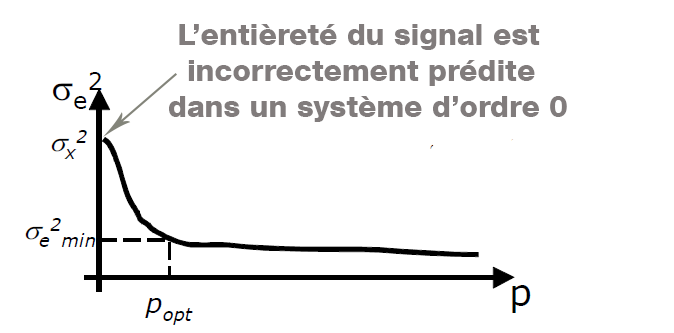
\includegraphics[scale=0.675]{Images/ordre_p}
				\end{figure}\noindent
			\end{minipage}

	\subsection{Extensions of the AR model}

		\paragraph{\red{Expliquer comment on synthétise un signal de parole avec le modèle LPC.}}~\\~\\
			\point On vient placer dans le filtre les coefficients qu'on a mesuré, et on remplace le
				\\\alinea résidu de prédiction par deux excitations type : 
				\begin{itemize}
					\setlength{\itemsep}{0pt}		
					\setlength{\parskip}{0pt}		
					\setlength{\parsep}{0pt}	
					\item Une suite d'impulsions de Dirac parfaitement périodique (voisé)
					\item Un bruit blanc (non voisé)
				\end{itemize}
				qui sont ensuite passés dans l'amplificateur $\sigma$.
		
		\paragraph{\red{Préciser les éléments du modèle sur lesquels agir pour améliorer la qualité du signal 
		~\\ \hspace*{0.035cm} modélisé.}}~\\~\\
			\point Les excitations d'entrée sont parfaitement arbitraires, et c'est elles qu'il faut tenter
				\\\alinea d'améliorer pour améliorer la qualité du signal produit.
		
		\paragraph{\red{Citer deux types de problèmes typiques de l'analyse LPC.}}~\\~\\
			\begin{itemize}
				\setlength{\itemsep}{0pt}		
				\setlength{\parskip}{0pt}		
				\setlength{\parsep}{0pt}	
				\item Problème des anti-formants (nasaux par exemple)
				\item Problème des sons mixtes (exemple : son $vv$)
			\end{itemize}
		
		\paragraph{\red{Définir ce qu'est un anti-formant et préciser son origine dans le système naturel de 
		~\\ \hspace*{0.035cm} production de la parole.}}~\\~\\
			\point \myul{Anti-formant} : Signaux émis en opposition de phase qui fait que le contenu fréquentiel
				\\\alinea est très faible (\hl{2 signaux proches qui s'annulent pour une fr\'equence donn\'ee}).\\
			\begin{minipage}{0.45\textwidth}
				\begin{figure}[H]
				\centering
				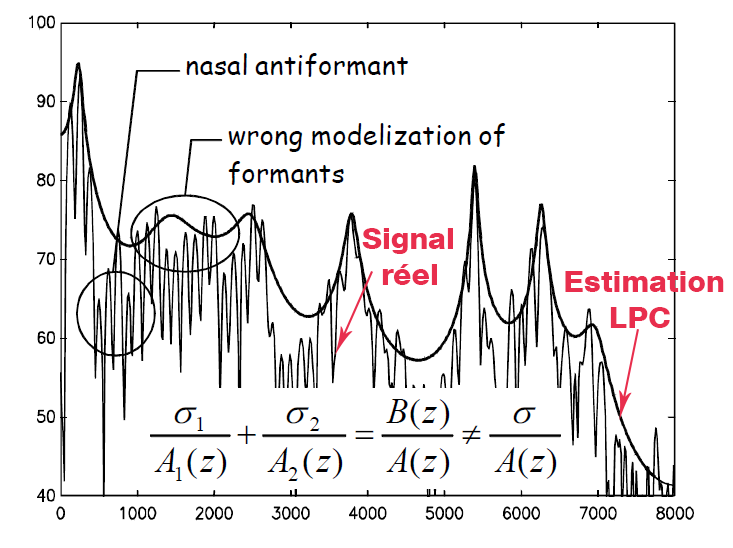
\includegraphics[scale=0.6]{Images/antiformants}
			\end{figure}\noindent
			\end{minipage}\hfill
			\begin{minipage}{0.45\textwidth}
				\alinea La distance a parcourir et la différence du conduit entre le nez et la bouche peuvent
					causer un déphasage qui annule le signal total (somme des deux).				
				\\
				\alinea \'Etant donné que le modèle LPC est un \hl{mod\`ele tous p\^oles} (capable de reproduire des
					formants), il est \hl{difficile de repr\'esenter un anti-formant par ce mod\`ele}.
			\end{minipage}
		
		\paragraph{\red{Préciser l'origine des sons mixtes dans le système naturel de production de la parole.}}~\\~\\
			\point \hl{Sons mixtes} : sons pour lesquels les cordes vocales entrent en vibration, mais pour lesquels
				\\\alinea les cordes vocales ne se ferment pas complètement. Ce qui donne un \hl{m\'elange entre un}
				\\\alinea \hl{signal vois\'e et un signal non-vois\'e}.\\
			\point On pourrait être tenté de remplacer l'interrupteur par une somme entre signal vois\'e et 
				\\\alinea non-vois\'e (ce qui existe comme mod\`ele), mais cela rend le mod\`ele excessivement
				complexe.
				
		\paragraph{\red{Rappeler l'idée de base du modèle MP-LPC.}}~\\~\\
			\point \myul{MultiPulse Linear Prediction (MP-LPC)} : Créé pour palier aux problèmes de modélisation
				\\\alinea du modèle LPC. Il remplace l'excitation à deux types du modèle LPC par quelque chose
				\\\alinea de beaucoup plus flexible : \hl{un petit nombre d'impulsions r\'eglables en position et 
				amplitude}.\\
			\begin{minipage}{0.4\textwidth}
				\begin{figure}[H]
					\centering
					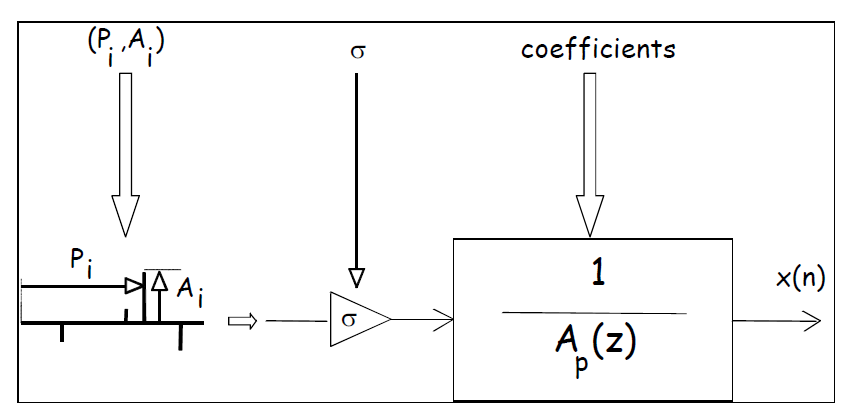
\includegraphics[scale=0.5]{Images/mp-lpc}
				\end{figure}\noindent
			\end{minipage}\hfill
			\begin{minipage}{0.43\textwidth}
				\alinea L'excitation est représentée par un \hl{petit nombre d'impulsions de Dirac} dont on peut 
					\hl{r\'egler la position et l'amplitude} de manière individuelle.
			\end{minipage}
		
		\paragraph{\red{Préciser comment estimer un modèle MP-LPC et expliquer la difficulté de cette estimation.}}~
		\\~\\
			\point On devrait \hl{imaginer toutes les excitations possibles}. Ce qui veut dire que pour chaque
				\\\alinea impulsion, il faudrait tester toutes les positions et les amplitudes possibles
				\\\alinea pour choisir les paramètres idéaux. Ce qui fait exploser le nombre de calculs.
		
		\paragraph{\red{Rappeler l'idée de base du modèle CELP et citer un problème de ce modèle.}}~\\~\\
			\point \myul{Code Excited Linear Prediction (CELP)} : Créé pour palier aux problèmes de modélisation
				\\\alinea du modèle LPC. Il remplace l'excitation à deux types du modèle LPC par quelque chose
				\\\alinea de plus flexible : on remplace l'interrupteur à deux positions du mod\`ele LPC par un
				\\\alinea \hl{interrupteur \`a 1024 ou 2048 positions.}\\
			\begin{minipage}{0.4\textwidth}
				\begin{figure}[H]
					\centering
					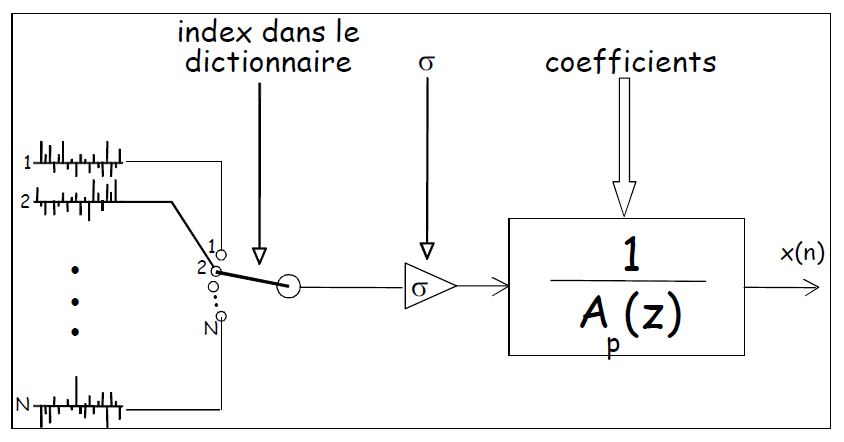
\includegraphics[scale=0.5]{Images/celp}
				\end{figure}\noindent
			\end{minipage}\hfill
			\begin{minipage}{0.43\textwidth}
				\alinea L'excitation est choisie parmi un assez grand nombre de signaux différents. \hl{On 
					consid\`ere qu'il y en aura au moins une qui conviendra.} La difficulté revient alors
					à choisir la bonne position de l'interrupteur.
			\end{minipage}
			\pagebreak
\section{Speech Coding}
	\subsection{Speech Coding}
		\paragraph{\red{Citer les deux buts fondamentaux du codage d'un signal de parole.}}
			\begin{itemize}	
				\item \hl{Stocker} du signal de la parole sur un espace de \hl{stockage minimal}
				\item \hl{Transmission} du signal de parole sur un canal à \hl{bande passante minimale}
			\end{itemize}
		
		\paragraph{\red{Expliquer pourquoi les algorithmes traditionnels de compression ne fonctionnent pas pour  
		~\\ \hspace*{0.035cm} un fichier de parole.}}~\\~\\
			\point Les systèmes de compression standards ne fonctionnent pas bien avec les fichiers sons.
				\\\alinea En effet, les algorithmes classiques (zip, rar, ...) recherche des suites de bytes
				\\\alinea qui se répètent. Dés lors, on ne stocke cette suite qu'une seule fois.
				\\\alinea Ceci n'arrive jamais dans un fichier audio. \hl{WAV} $\rightarrow$ \hl{On stocke des suites 
				de pression}
				\\\alinea acoustique à des moments très rapprochés. Et \hl{ces suites ne se r\'ep\`etent 
				presque jamais}.
		
		\paragraph{\red{Donner l'ordre de grandeur du débit binaire minimal d'un signal de parole (en ne  
		~\\ \hspace*{0.035cm} considérant que son contenu phonétique) et le comparer au débit binaire admissible  
		~\\ \hspace*{0.035cm} par une ligne téléphonique.}}~\\~\\
			\point \myul{Débit minimal} : Le nombre minimal de bits par seconde qui permettent de conserver
				\\\alinea l'information contenu dans le signal de parole : 
				\begin{itemize}
					\setlength{\itemsep}{0pt}		
					\setlength{\parskip}{0pt}		
					\setlength{\parsep}{0pt}	
					\item Contenu : suite de phonèmes qui constituent le message à faire passer.
					\item La voix de l'orateur : ce qui permet de reconnaître la voix de l'orateur.
					\item Le para-linguistique : l'intonation
				\end{itemize}
			\point On va se concentrer sur le stockage de contenu. On a vu qu'on a environ un phonème par 
				\\\alinea $0,1$s, donc 10 phonèmes par secondes. Le \hl{nombre de phon\`emes de la langue} 
				va d\'efinir
				\\\alinea le nombre de bits sur lesquels sont stocké le contenu (32 phonèmes = 5 bits).
				\\\alinea Pour l'exemple on a donc \hl{5 bits * 10 phon\`emes/s = 50 bits/s}.\\
			\point Les lignes téléphoniques permettent l'échange de parole à environ 50kbits/s. On a donc
				\\\alinea 1000 fois le débit minimal.
				
		
		\paragraph{\red{Décrire en les illustrant par un schéma, la technique de quantification uniforme et  
		~\\ \hspace*{0.035cm} l'erreur de quantification qui lui est liée.}}~\\~\\
			\point \myul{Quantification} : op\'eration consistant \`a \hl{remplacer les valeurs continues} mesur\'ees
				\\\alinea par l'ordinateur \hl{par des valeurs discr\`etes}. Elle est caract\'eris\'ee par un
				\\\alinea nombre de bits $b$, qui défini le nombre de pas de la fonction escalier \`a $2^b$.\\
			\point \myul{Quantification uniforme} : quantification dans laquelle la taille des escaliers est
				\\\alinea constante.\\
			\begin{minipage}{0.65\textwidth}
				\begin{figure}[H]
					\centering
					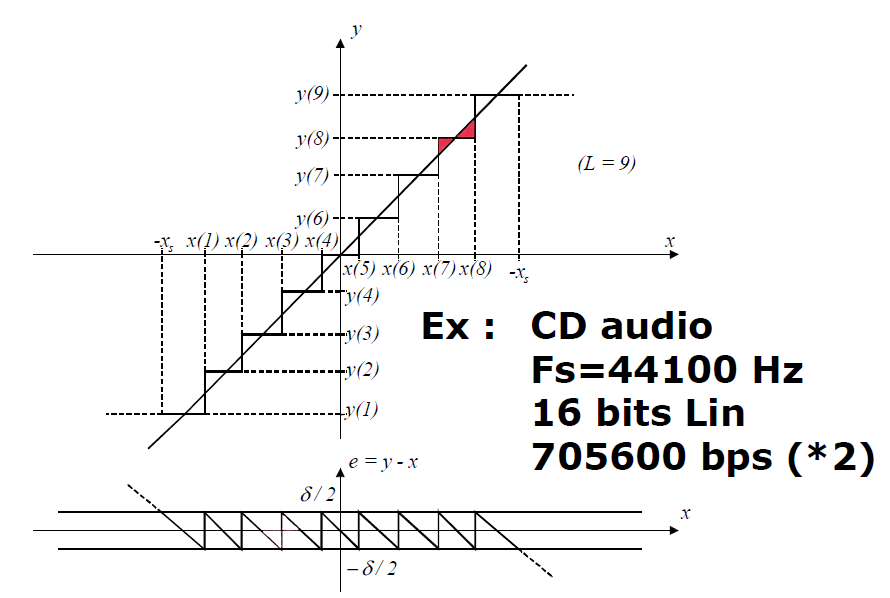
\includegraphics[scale=0.6]{Images/uquantization}
				\end{figure}\noindent
			\end{minipage}\hfill
			\begin{minipage}{0.38\textwidth}
				\point L'\myul{erreur liée à la quantification} est la \hl{diff\'erence entre la sortie discr\`ete et 
					l'entr\'ee continue} (cf. triangle rouge). Plus $b$ est grand, au plus l'erreur est petite.
			\end{minipage}
		
		\paragraph{\red{Détailler l'emploi de la technique de quantification uniforme pour un CD audio et calculer  
		~\\ \hspace*{0.035cm} le débit binaire correspondant.}}~\\~\\
			\point Voir image ci-dessus, On utilise $b$ = 16bits, et \ \ \ 44100Hz $\cdot$ 16bits = 705600bits/s.
				\\\alinea et comme on a des sons stéréo, on peut multiplier ce nombre par deux.
				\\\alinea Ce n'est donc pas un codeur de ce type qui est utilisé pour les CD mais plutôt
				\\\alinea un codage éliminant les composantes sonores inaudibles du fait de l'effet de masquage 
				\\\alinea fréquentiel.
		
		\paragraph{\red{Détailler l'emploi de la technique de quantification uniforme pour le codage de parole.}}
		~\\
			\begin{minipage}{0.6\textwidth}
				\begin{figure}[H]
					\centering
					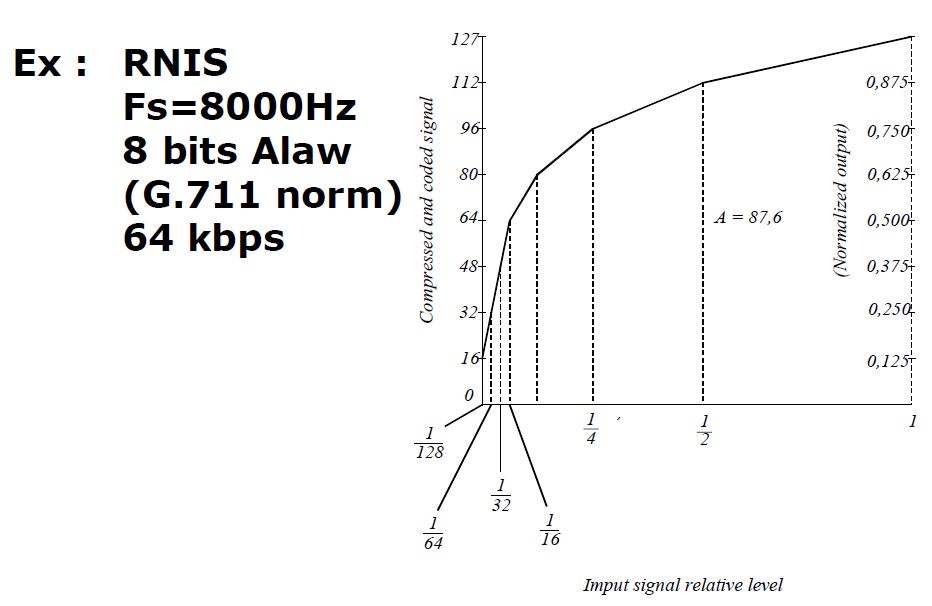
\includegraphics[scale=0.5]{Images/nuquantization}
				\end{figure}\noindent
			\end{minipage}\hfill
			\begin{minipage}{0.35\textwidth}
				\point Le signal de parole utilisant beaucoup plus de petites valeurs que de grandes, 
					on va préférer un système de quantification non linéaire, qui permet d'être \hl{plus pr\'ecis dans
					les petites valeurs.}
			\end{minipage}
		
		\paragraph{\red{Expliquer le principe d'une compression selon la loi A et citer une technologie qui 
		~\\ \hspace*{0.035cm} l'exploite.}}~\\~\\
			\point Cette compression permet d'obtenir une bonne qualité audio en prenant $b$ = 8bits et $f$ = 8kHz. \\
			\point Utilisée dans le RNIS : codage et décodage entre deux centrales téléphoniques.
	
	\subsection{Coders}
		
		\paragraph{\red{Schématiser un codeur par prédiction linéaire et commenter son fonctionnement.}}~\\
		\begin{minipage}{0.4\textwidth}
			\begin{enumerate}
				\setlength{\itemsep}{0pt}		
				\setlength{\parskip}{0pt}		
				\setlength{\parsep}{0pt}
				\item Algorithme de Shchur afin de devnier les \hl{coefficients} de prédiction.
				\item Analyse de \hl{fr\'equence fondamentale}.
				\item Décision signal \hl{vois\'e/non-vois\'e}.
				\item \hl{Transmission} (100 fois/s) des coefficients, de la période et l'information 
					voisé/non-voisé. Le tout en \hl{24bits}.
				\item \hl{D\'ecodage} par synthétiseur LPC
			\end{enumerate}
		\end{minipage}\hfill
		\begin{minipage}{0.55\textwidth}
			\begin{figure}[H]
				\centering
				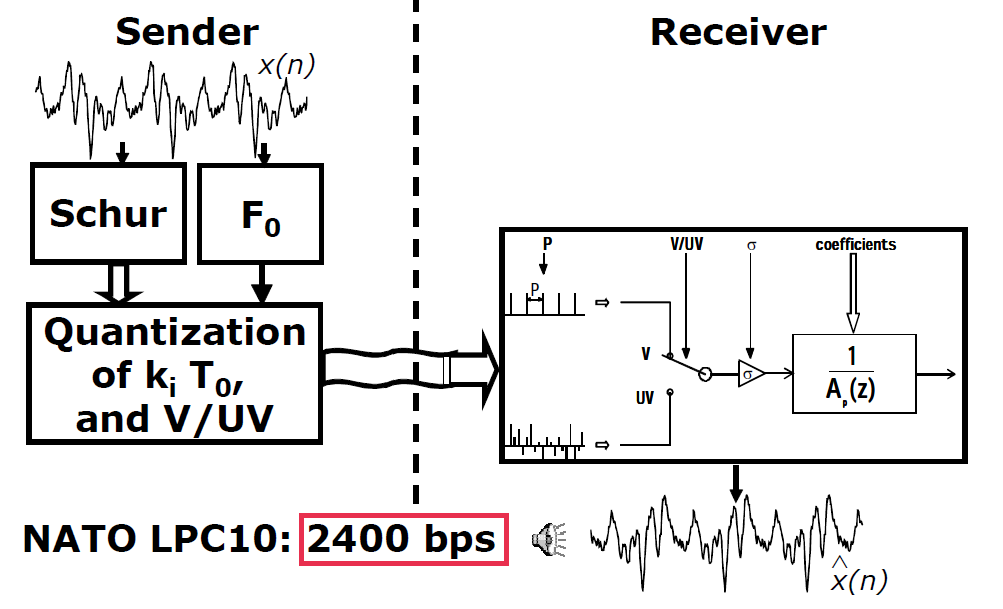
\includegraphics[scale=0.5]{Images/coder-lpc}
			\end{figure}\noindent
		\end{minipage}
		\paragraph{\red{Citer la caractéristique typique de la parole codée en respectant la norme LPC10 et 
		~\\ \hspace*{0.035cm} donner un exemple d'emploi dans la vie courante.}}~\\~\\
			\point On y entend un caractère distordu\hl{ m\'etallique}. De plus, une mauvaise d\'ecision 
				\\\alinea vois\'e/non-vois\'e peut causer qu'un $sss$ se transforme en $zzz$ après codage/décodage.\\
			\point Les \hl{transmissions par satellites} sont normalisées en LPC10.
			
		\paragraph{\red{Schématiser un codeur MP-LPC et commenter son fonctionnement.}}~\\
			\begin{minipage}{0.55\textwidth}
				\begin{figure}[H]
					\centering
					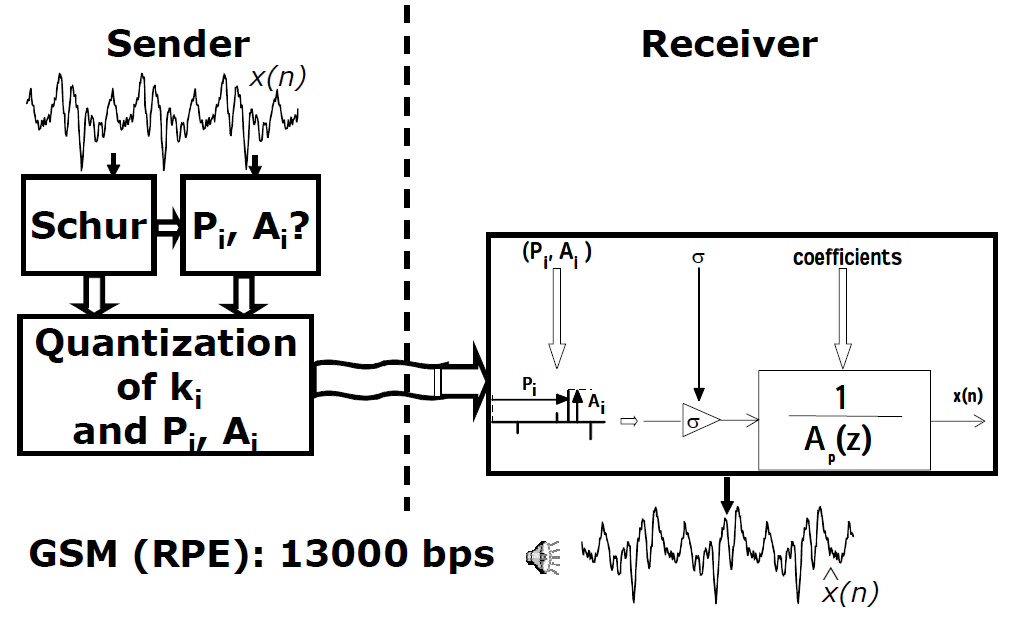
\includegraphics[scale=0.35]{Images/coder-mplpc}
				\end{figure}\noindent
			\end{minipage}\hfill
			\begin{minipage}{0.4\textwidth}
				\begin{enumerate}
					\setlength{\itemsep}{0pt}		
					\setlength{\parskip}{0pt}		
					\setlength{\parsep}{0pt}	
					\item Algorithme de \hl{Schur}.
					\item Estimation de la \hl{position} et de l'\hl{amplitude} du modèle.
					\item \hl{Transmission} et quantification de ces grandeurs.
					\item \hl{D\'ecodage} par synthétiseurs MP-LPC
				\end{enumerate}
			\end{minipage}
		\paragraph{\red{Justifier la dégradation de la parole lors d'une communication par GSM.}}~\\~\\
			\point La norme RPE est un modèle simplifié du modèle MP-lPC. La dégradation est due au fait
				\\\alinea qu'on n'entend pas vraiment l'interlocuteur mais un synthétiseur de voix
				\\\alinea qui fait de son mieux pour reproduire le signal vocal. \\
			\point De plus, le fait de deviner les coefficients implique la résolution d'un système de 10
				\\\alinea équations à 10 inconnues 10 fois par seconde. 
		
		\paragraph{\red{Schématiser un codeur CELP et commenter son fonctionnement.}}~\\
			\begin{minipage}{0.4\textwidth}
				\begin{enumerate}
					\setlength{\itemsep}{0pt}		
					\setlength{\parskip}{0pt}		
					\setlength{\parsep}{0pt}	
					\item Algorithme de \hl{Schur}.
					\item Estimation de l'indice du dictionnaire d'excitation du modèle.
					\item \hl{Transmission} et quantification de ces grandeurs en 48 bits.
					\item \hl{D\'ecodage} par synthétiseurs CELP
				\end{enumerate}
			\end{minipage}\hfill
			\begin{minipage}{0.55\textwidth}
				\begin{figure}[H]
					\centering
					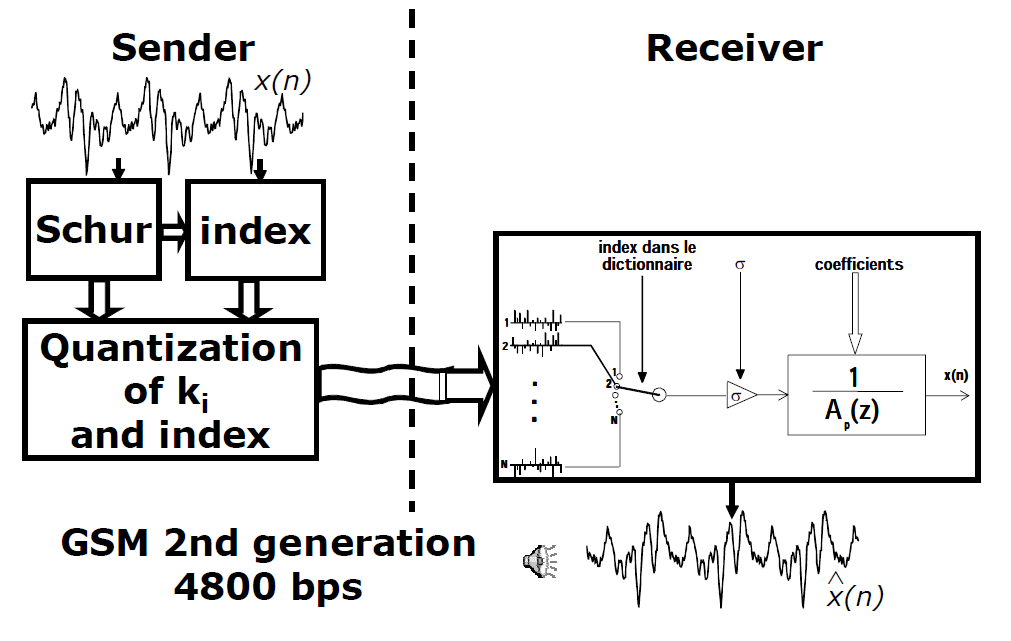
\includegraphics[scale=0.35]{Images/coder-celp}
				\end{figure}\noindent
			\end{minipage}
		\paragraph{\red{Expliquer l'avantage que procure l'UMTS sur le GSM en ce qui concerne la transmission 
		~\\ \hspace*{0.035cm} de la voix.}}~\\~\\
			\point Il n'a besoin que de 10 bits par $0,1s$ pour les coefficients du système d'équations.
				\\\alinea \hl{Le reste disponible peut \^etre utilis\'e pour stocker l'indice du dictionnaire.}
				\\\alinea (1024 positions = 10 bits $\rightarrow$ 38 bits = beaucoup !) 
		%
	\subsection{Conclusion}
		%
		\paragraph{\red{Positionner sur un schéma qualité/débit les techniques de codage de parole.}}~\\
			\begin{figure}[H]
				\centering
				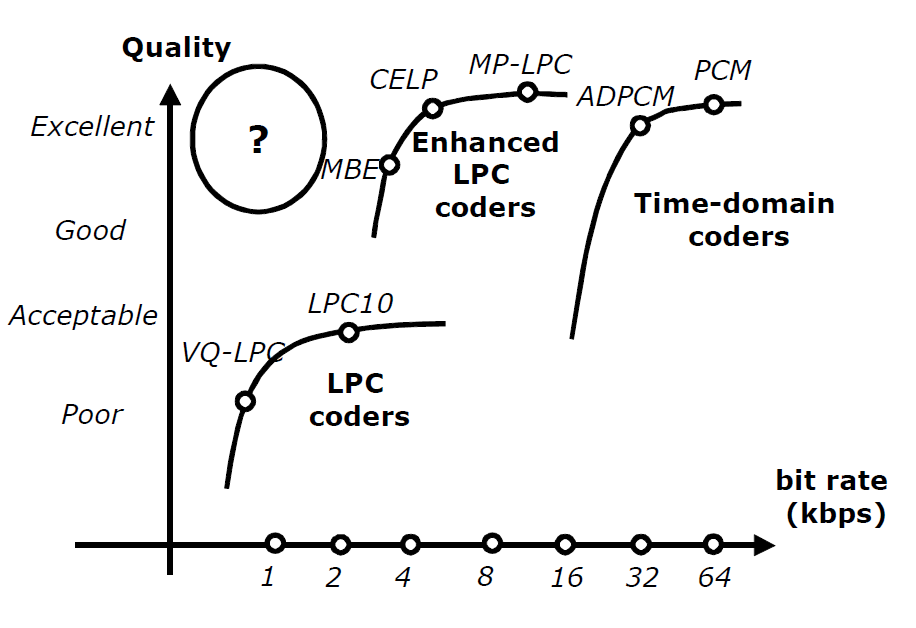
\includegraphics[scale=0.375]{Images/quality}
			\end{figure}\noindent
		\paragraph{\red{Citer une restriction importante à opérer sur le signal de parole traité, pour espérer 
		~\\ \hspace*{0.035cm} un jour coder la parole avec un très bas débit (moins de 200 bits/s).}}~\\~\\
			\point Il faudrait que les codeurs soient des codeurs phonétiques. C'est-\`a-dire qu'ils doivent
				\\\alinea \hl{savoir quelle langue ils codent/d\'ecodent}. Ce qui est pour le moment impossible à
				\\\alinea automatiser.
			
		\paragraph{\red{Prédire l'avenir de la recherche en codage de parole et justifier cette prédiction.}}~\\~\\
			\point\hl{ Tout ce qui devait \^etre trouv\'e en codage de la parole a d\'ej\`a \'et\'e trouv\'e}.
				\\\alinea la seule manière d'améliorer les techniques existantes seraient de surmonter
				\\\alinea la restriction citée ci-dessus.
\pagebreak		
\section{Automatic Speech Recognition}
	\subsection{Notes du présentiel}
		%
		\paragraph{\green{}}
		
		%
		\paragraph{\green{}}
		
		%
		\pagebreak
	\subsection{Automatic Speech Recognition (ASR)}
		%
		\paragraph{\red{Justifier, sur le plan économique, le développement des systèmes de reconnaissance 
		~\\ \hspace*{0.035cm} de parole.}}~\\~\\
			\point Les \hl{soci\'et\'es de t\'el\'ecomunication} sont les sponsors principaux de la recherche
				\\\alinea dans la reconnaissance automatique de la parole. En effet, ces sociétés s'intéressent
				\\\alinea à offrir des services payants à leurs clients en impliquant le moins d'employés
				\\\alinea possible. L'automatisation de la reconnaissance de la parole permet ce genre de services.
			\begin{itemize}
				\setlength{\itemsep}{0pt}		
				\setlength{\parskip}{0pt}		
				\setlength{\parsep}{0pt}	
				\item Secrétaire virtuelle : pouvoir parler à un robot qui prend des rendez-vous, qui vous connait,
					...
				\item Traduction automatique : pouvoir parler en anglais et l'ordinateur le répète en mandarin.
			\end{itemize}
			\point L'\hl{arm\'ee am\'ericaine} a subsidié aussi cette recherche dans le but de pouvoir traduire 
				l'anglais américain vers de dialectes arabes.
		
		\paragraph{\red{Donner trois domaines d'application de la reconnaissance de parole, ainsi qu'un 
		~\\ \hspace*{0.035cm} exemple pratique pour chacun de ces domaines.}}
			\begin{itemize}
				\setlength{\itemsep}{0pt}		
				\setlength{\parskip}{0pt}		
				\setlength{\parsep}{0pt}	
				\item \hl{Bureau} : contrôle vocal d'un ordinateur, d'une prise de note. (Un peu abandonné...)
				\item \hl{Business} : gérer des stocks, en disant ce qu'il manque/reste à un ordinateur. 
					(Un peu	abandonné...)
				\item \hl{M\'edical} : système de reconnaissance de mot clé pour rédaction automatique
					de rapport (Encore en développement actif !).
				\item \hl{Traduction} : traduire d'une langue en une autre rien qu'en entendant la parole. 
					(Encore en développement
					actif !).
			\end{itemize}
		
		\paragraph{\red{Expliquer pourquoi la coarticulation représente un important défi de la reconnaissance 
		~\\ \hspace*{0.035cm} de parole.}}~\\~\\
			\point \myul{Rappel -- coarticulation} : lorsqu'on prononce deux fois le même son dans deux mots 
				\\\alinea différents, ils seront différents. Car le son dépend du son émis précédemment et 
				\\\alinea des son à émettre prochainement.\\
			\point \hl{On peut donc avoir du mal \`a reconna\^itre les sons}, car les zones de prononciation
				\\\alinea des phonèmes se recouvrent. De plus, selon la personne qui parle, les zones de 
				\\\alinea recouvrements changent selon l'orateur.\\
			Les autres défis sont :
			\begin{itemize}
				\setlength{\itemsep}{0pt}		
				\setlength{\parskip}{0pt}		
				\setlength{\parsep}{0pt}	
				\item Différence des conduits vocaux
				\item Genre, dialecte
				\item Différence entre les langues
				\item Bruit ambiant, dû à l'environnement ou bruit humain.
			\end{itemize}
		
		\paragraph{\red{Citer la plus importante faiblesse des systèmes de reconnaissance de parole actuels.}}~\\~\\
			\point \myul{La robustesse au bruit} : capacit\'e \`a ne pas consid\'erer le bruit comme un probl\`eme.
		
		\paragraph{\red{Citer et définir les deux principaux types de bruit, donner deux exemples par type.}}
			\begin{itemize}
				\setlength{\itemsep}{0pt}		
				\setlength{\parskip}{0pt}		
				\setlength{\parsep}{0pt}	
				\item Bruit additif : bruit s'ajoutant au signal de la parole (applaudissement, 
					bruit dans le speaker du téléphone, ...). 
					Le cerveau reconstitue de lui-même les parties qui n'ont pas été entendues.
				\item Bruit convolutif : bruit qui est dû à l'\hl{environnement} se trouvant 
					\hl{entre le conduit vocal
					de l'orateur et le conduit auditif du destinataire} (réverbérations, distance, ...). 
					Dans un sens, on change le filtre, la fonction de transfert de la parole.
					Les bruit dûs à la qualité du canal téléphonique sont des bruits de convolution car le 
					signal est envoyés par une ligne différente entre chaque appel.
				\item Bruit inter-orateur : bruit dû au stress, à l'âge, à l'humeur, à l'effet Lombard...
			\end{itemize}
		
		\paragraph{\red{Donner une idée de ce qu'est l'effet Lombard.}}~\\
			\point \myul{L'effet Lombard} : le cerveau est constamment en train d'écouter le bruit ambiant afin
				\\\alinea de savoir si ce que l'on va dire va bien être transmis au destinataire ou pas.
				\\\alinea Il y a donc une boucle de rétroaction (feedback) qui va permettre au cerveau d'\hl{adapter}
				\\\alinea \hl{la transmission de certains sons selon le bruit ambiant}.
		%
	\subsection{ASR Systems}
		%
		\paragraph{\red{Énoncer les contraintes qui régissent le choix d'un système de reconnaissance de parole.}}
		~\\
			\begin{itemize}
				\setlength{\itemsep}{0pt}		
				\setlength{\parskip}{0pt}		
				\setlength{\parsep}{0pt}	
				\item \hl{D\'ependant} ou ind\'ependant du locuteur.
				\item Type de reconnaissance : 
					\begin{itemize}
						\setlength{\itemsep}{0pt}		
						\setlength{\parskip}{0pt}		
						\setlength{\parsep}{0pt}	
						\item Reconnaissance par \hl{mot isol\'e} $\rightarrow$ Mettre des blancs volontairement 
							entre les différents mots pour faciliter la segmentation de la phrase
						\item Reconnaissance par \hl{mots connect\'es} $\rightarrow$ Apparent à la reconnaissance
							par mots clés.
						\item Reconnaissance de \hl{parole continue} $\rightarrow$ Le plus compliqué car doit 
							diviser la phrase en mots
						\item Reconnaissance de \hl{mots cl\'es} $\rightarrow$ Ce qui est fait intuitivement quand on 
							écoute une langue étrangère.
					\end{itemize}
				\item Taille du vocabulaire connu. Petit : 100 mots; Moyen : 5000 mots; Grand : 50000 mots.
				\item Perplexité : le nombre de mots moyen qui pourrait suivre un mot.
				\item Contraintes de robustesse (conditions de laboratoire à conditions réelles) : 
					\begin{itemize}
						\setlength{\itemsep}{0pt}		
						\setlength{\parskip}{0pt}		
						\setlength{\parsep}{0pt}	
						\item Bruit ambiant. 
						\item Type et qualité du microphone.
						\item Position du micro.
					\end{itemize}
			\end{itemize}
		%
		\paragraph{\red{Positionner la complexité d'un système de reconnaissance de parole par rapport à un autre 
		~\\ \hspace*{0.035cm} en fonction de leurs contraintes.}}~\\
			\begin{figure}[H]
				\centering
				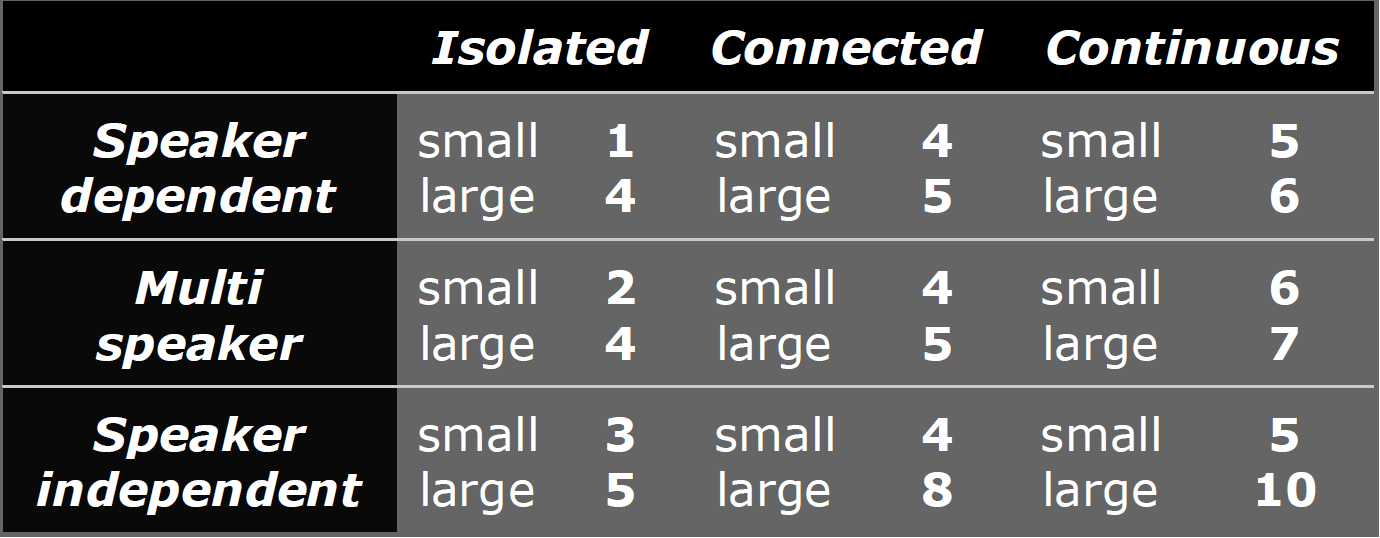
\includegraphics[scale=0.25]{Images/complexity}
			\end{figure}\noindent
		%
		\paragraph{\red{Schématiser et commenter les principes de fonctionnement des trois grandes familles 
		~\\ \hspace*{0.035cm} de reconnaisseurs de parole étudiés depuis les années 60.}}~\\~\\
			\begin{minipage}{0.4\textwidth}
				\begin{figure}[H]
					\centering
					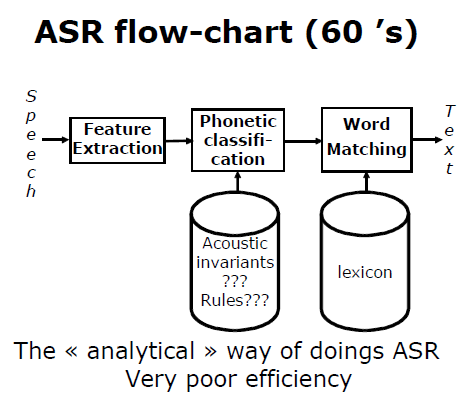
\includegraphics[scale=0.45]{Images/60s}
				\end{figure}\noindent
			\end{minipage}\hfill
			\begin{minipage}{0.55\textwidth}
				\point Extraire les \hl{formants} par LPC et en déduire le son produit. 
					Ce reconnaisseur était régit par des règles de type \textit{Si, Alors}. \\~\\
				\point Idée: implémenter l'expertise d'un spécialiste de la
					parole qui sait lire un spectrogramme. De bonnes règles n'ont jamais été trouvées.
			\end{minipage}~\\
			\begin{minipage}{0.55\textwidth}
				\point Approche basée sur des \hl{exemples}. On stocke la suite des vecteurs donnés par l'analyse
					LPC. Ces vecteur sont soumis à une comparaison par rapport à un fichier exemple.
					Si le résultat de la comparaison est bon, on admet que c'est le même mot.\\~\\
				\point Demande un petit vocabulaire et d'être dépendant du locuteur.
			\end{minipage}\hfill
			\begin{minipage}{0.4\textwidth}
				\begin{figure}[H]
					\centering
					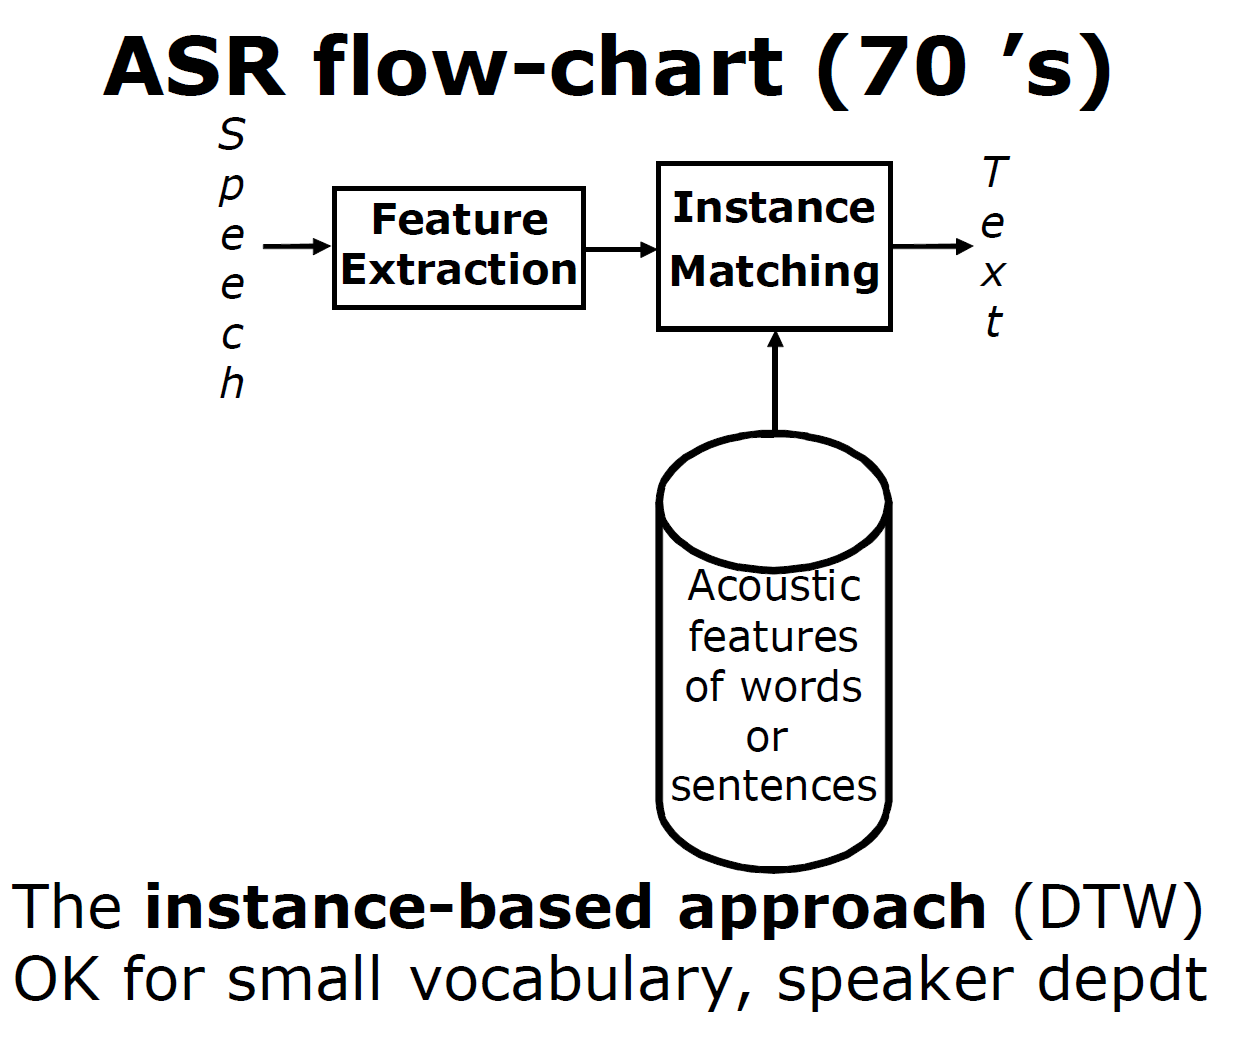
\includegraphics[scale=0.2]{Images/70s}
				\end{figure}\noindent
			\end{minipage}~\\
			\begin{minipage}{0.4\textwidth}
				\begin{figure}[H]
					\centering
					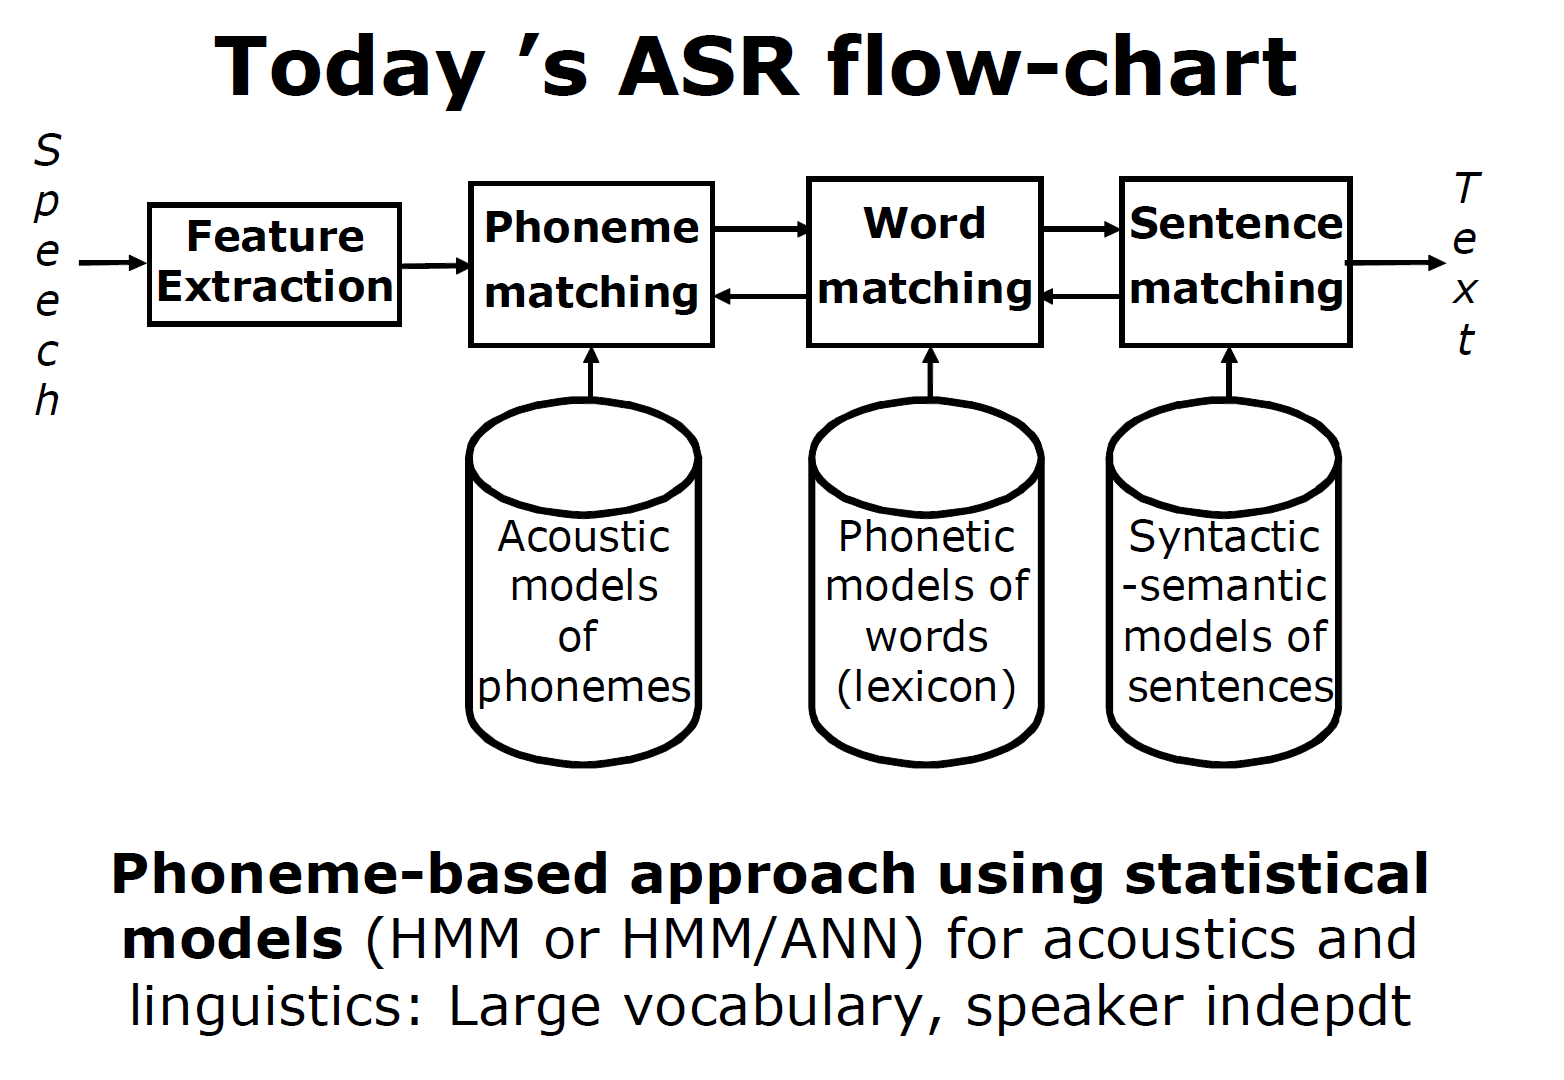
\includegraphics[scale=0.235]{Images/TODAYs}
				\end{figure}\noindent
			\end{minipage}\hfill
			\begin{minipage}{0.55\textwidth}
				\point Approche basée sur des modèles statistiques. On compare les vecteurs donnés par LPC
					et on les compare avec un modèle qui donne un degrés de certitude de match.\\~\\
				\point Ceci est d'abord réalisé pour des phonèmes et ensuite pour des mots, et enfin pour 
					des phrases. C'est cette reconnaissance de phrases qui va émettre une conclusion.\\~\\
				\point Les deux derniers blocs vont chercher le meilleur chemin parmi ceux qui sont possibles
					grâce à l'analyse précédente.
			\end{minipage}
		%
		\paragraph{\red{Expliquer quels types de connaissances embarque un système de reconnaissance basée sur 
		~\\ \hspace*{0.035cm} des modèles statistiques.}}~\\
			\vspace*{-0.45cm}
			\begin{itemize}
				\setlength{\itemsep}{0pt}		
				\setlength{\parskip}{0pt}		
				\setlength{\parsep}{0pt}	
				\item Connaissances acoustiques : quel son a du sens pour la langue.
				\item Connaissances lexicales : quel mot fait ou ne fait pas parti de la langue.
				\item Connaissances sémantiques/syntaxiques : quelle phrase a du sens dans la langue.
			\end{itemize}		
		%		
		\paragraph{\red{Préciser les contextes d'utilisations respectifs (en fonction des contraintes qui régissent 
		~\\ \hspace*{0.035cm} le choix d'un système de reconnaissance) de la de la reconnaissance basée sur des 
		modèles ~\\ \hspace*{0.035cm} et de celle basée sur des modèles statistiques.}}~\\
			\vspace*{-0.45cm}
			\begin{itemize}
				\setlength{\itemsep}{0pt}		
				\setlength{\parskip}{0pt}		
				\setlength{\parsep}{0pt}	
				\item Modèle: besoin de stocker tous les exemples en mémoire afin de les comparer un à un. 
					Fonctionne bien avec un \hl{petit vocabulaire} et en étant \hl{d\'ependant du locuteur}.
				\item Statistiques: besoin d'un seul modèle statistique pour tout reconnaitre (ou essayer du moins).
					Correspond aux contraintes \hl{grand vocabulaire} et \hl{ind\'ependant de l'interlocuteur}.
			\end{itemize}
		%
	\subsection{Instance-based ASR}
		\paragraph{\red{Préciser le problème de base d'un système de reconnaissance basé sur des exemples et 
		~\\ \hspace*{0.035cm} présenter la solution généralement employée.}}~\\
			\begin{minipage}{0.4\textwidth}
				\point Le principe est de calculer le résultat d'une fonction $D$ de distance
				entre l'entrée et tous les exemples et on va associer l'entrée à l'exemple qui 
				a donné le plus petit résultat pour $D$.\\
			\end{minipage}\hfill
			\begin{minipage}{0.55\textwidth}
				\begin{figure}[H]
					\centering
					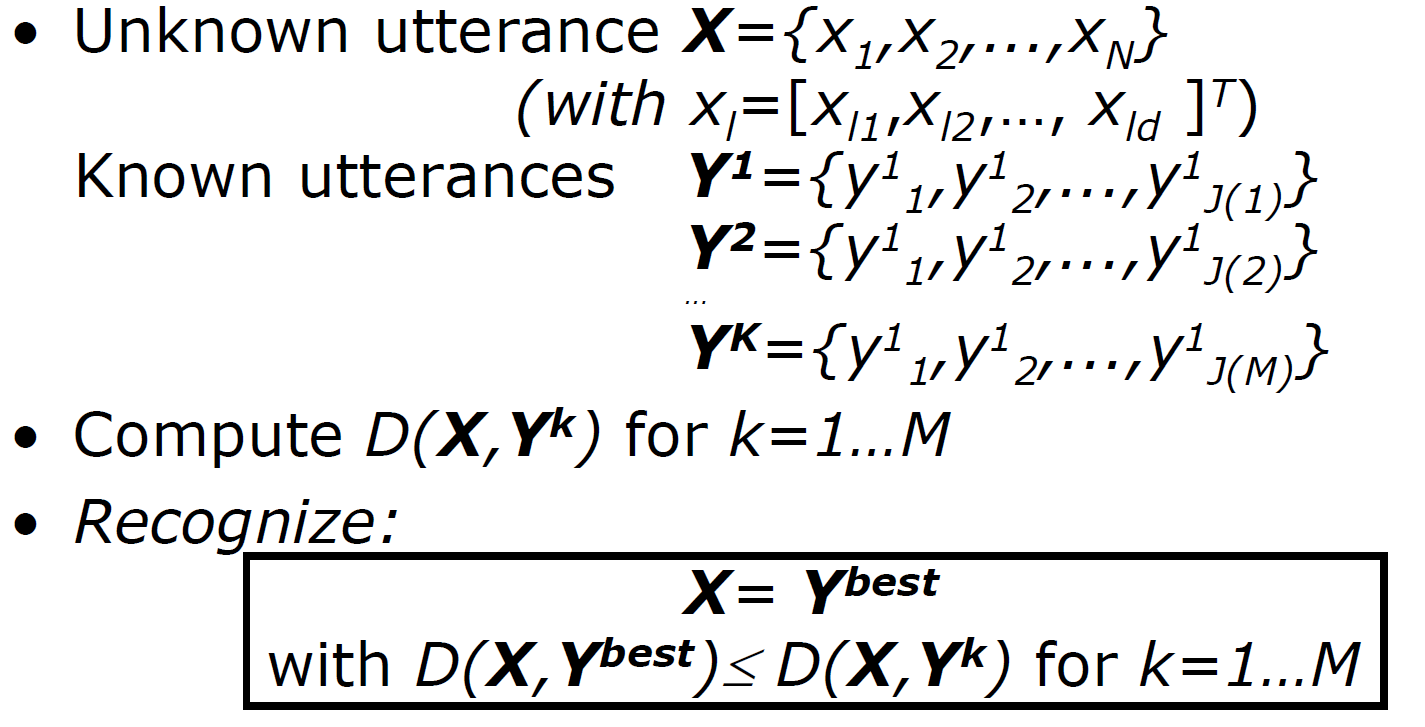
\includegraphics[scale=0.25]{Images/instance_based}
				\end{figure}\noindent
			\end{minipage}~\\
			\point \myul{Problème de base} : il est impossible de reproduire la même durée d'élocution pour 
				\\\alinea un même mot entre deux élocutions différentes $\rightarrow$ On a pas le même nombre de 
				\\\alinea vecteurs entre l'entrée et les exemples.
		
		\paragraph{\red{Préciser la notion de distance locale et de distance globale dans le cadre d'un système 
		~\\ \hspace*{0.035cm} de reconnaissance basé sur des exemples.}}~\\~\\
			\point \myul{Distance locale} : distance qui sépare un quelconque vecteur de l'entrée avec un quelconque 
				\\\alinea vecteur d'un exemple. Ces vecteurs sont de même tailles (car même analyse à l'origine).
				\\\alinea Plus simple à calculer : distance euclidienne. Il en existe d'autre ciblée au TDP.\\
			\point \myul{Distance globale} : On fait correspondre les vecteurs de l'entrée avec les vecteurs
				\\\alinea du mot de référence, et on calcule la distance entre ces correspondance et une
				\\\alinea courbe de base.
		%					
    	\paragraph{\red{Schématiser la solution la plus adéquate au problème du calcul de la distance globale 
    	~\\ \hspace*{0.035cm} dans le cadre de la reconnaissance basé sur des exemples, lorsque les mots à 
    	~\\ \hspace*{0.035cm} reconnaître sont longs.}}~\\~\\
    		\begin{minipage}{0.4\textwidth}
				\point Fait correspondre chaque vecteur de l'entrée avec chaque vecteur d'un exemple et
					calcule la distance entre cette correspondance et une correspondance linéaire "parfaite".\\~\\
				\point Pas réaliste car suppose une grande probabilité de \hl{correspondance parfaite}, ou du moins
					un \hl{allongement uniforme} entre l'entrée et l'exemple ce qui n'est pas possible car des sons
					comme $d$ ne s'allonge pas.
			\end{minipage}\hfill
			\begin{minipage}{0.55\textwidth}
				\begin{figure}[H]
				 	\centering
				 	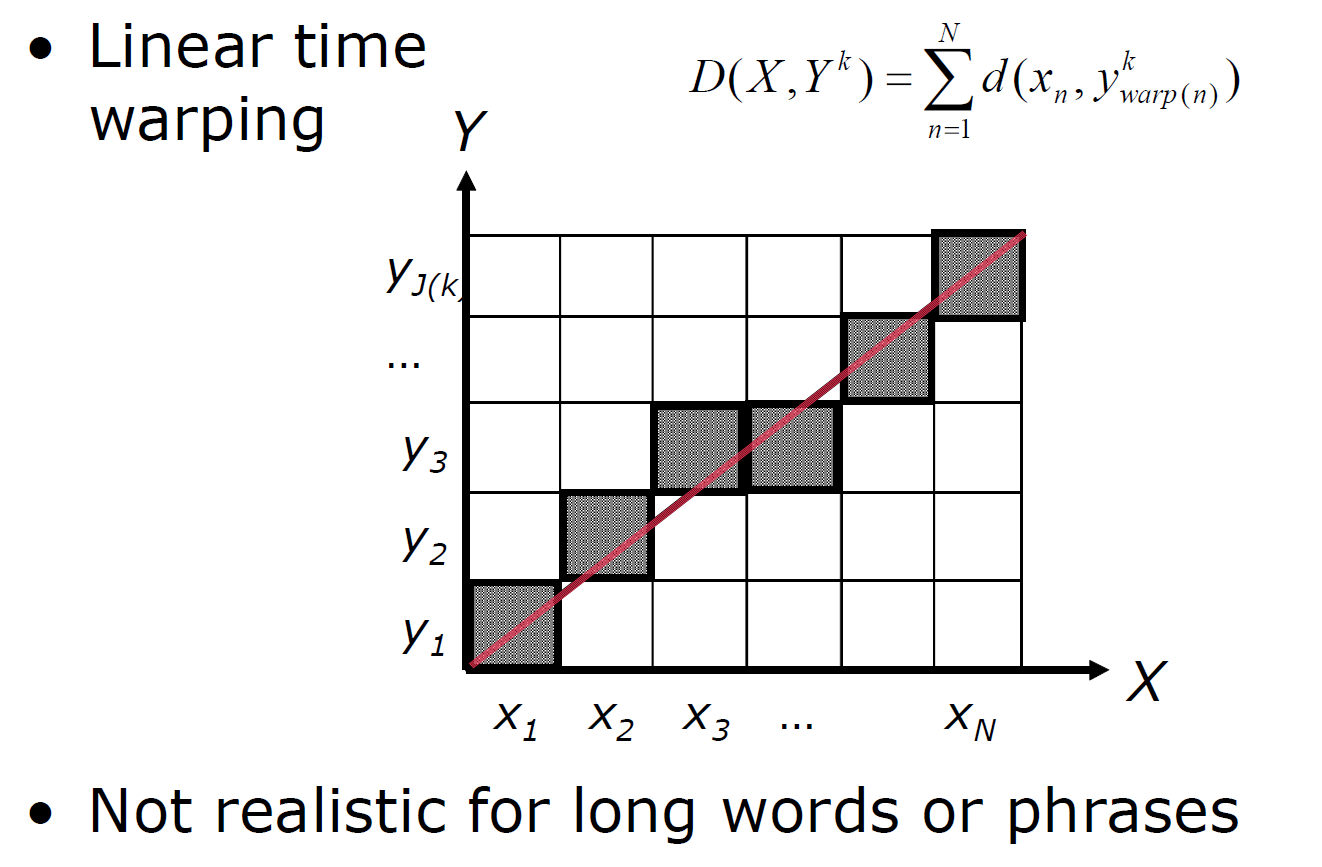
\includegraphics[scale=0.25]{Images/linear_time_wrapping}
				 \end{figure}\noindent 
			\end{minipage}~\\
			\begin{minipage}{0.55\textwidth}
				\begin{figure}[H]
					\centering
					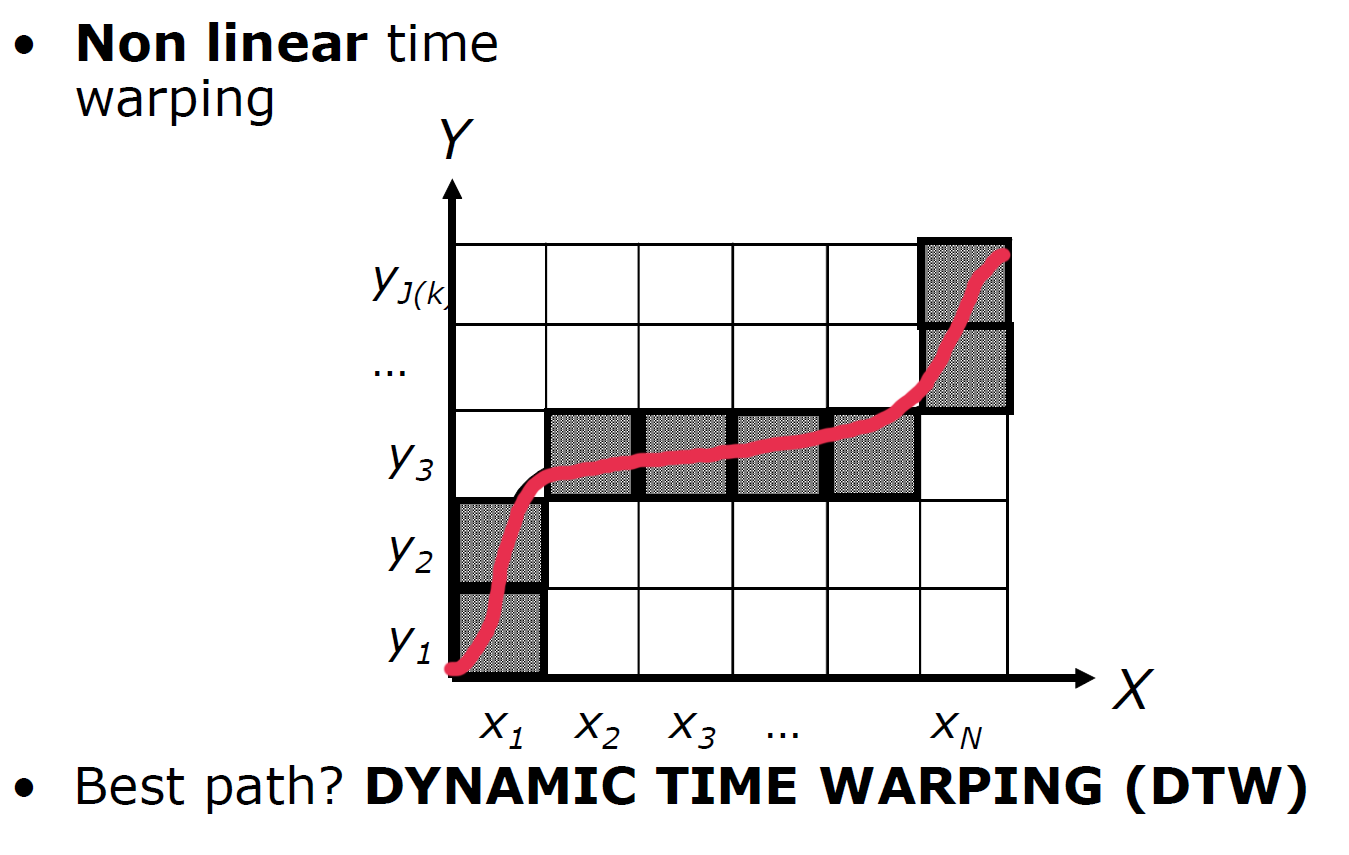
\includegraphics[scale=0.25]{Images/nonlinear_time_wrapping}
				\end{figure}\noindent
			\end{minipage}\hfill
			\begin{minipage}{0.4\textwidth}
				\point Cette fois, on suppose que \hl{certaines zones} de l'entrée sont répétées \hl{plus longtemps}
					que dans l'exemple et que d'\hl{autres zones} durent le \hl{m\^eme temps}.
			\end{minipage}
		
		\paragraph{\red{Expliquer conceptuellement l'algorithme DTW.}}~\\~\\
			\point \myul{DTW} : On examine toutes les courbes de référence possible, et pour tous ces chemins,
				\\\alinea on calcule la distance globale avec la correspondance expérimentale et on garde la 
				\\\alinea courbe qui représente la distance globale minimale.
		
		%	
	\subsection{Model-based ASR}
		\paragraph{\red{Présenter la classification bayesienne et définir les termes de la règle de Bayes dans 
		~\\ \hspace*{0.035cm} le cadre de la reconnaissance basée sur des modèles.}}~\\~\\
			\point Le principe est de supposer que l'entrée correspond à un des modèle présent en mémoire.
				\\\alinea Ce faisant, on suppose que l'ensemble des sons qu'il est possible de reconnaitre est
				\\\alinea fini, ce qui n'est en réalité pas le cas. Ensuite, le but est de calculer, pour chaque
				\\\alinea modèle, la probabilité que l'entrée corresponde à ce modèle.\\~\\
			%
			\begin{minipage}{0.4\textwidth}
				\point On parle de classification Bayésienne lorsqu'on utilise une classification \textit{a posteriori},
					c'est à dire lorsqu'on \hl{compare ce qui a voulu \^etre dit par rapport 
					\`a ce qui a \'et\^'e dit}.\\~\\
				\point Le problème est qu'il est impossible en pratique de connaître cette probabilité. On va donc
					utiliser la règle de Bayes.
			\end{minipage}\hfill
			\begin{minipage}{0.55\textwidth}
				\begin{figure}[H]
					\centering
					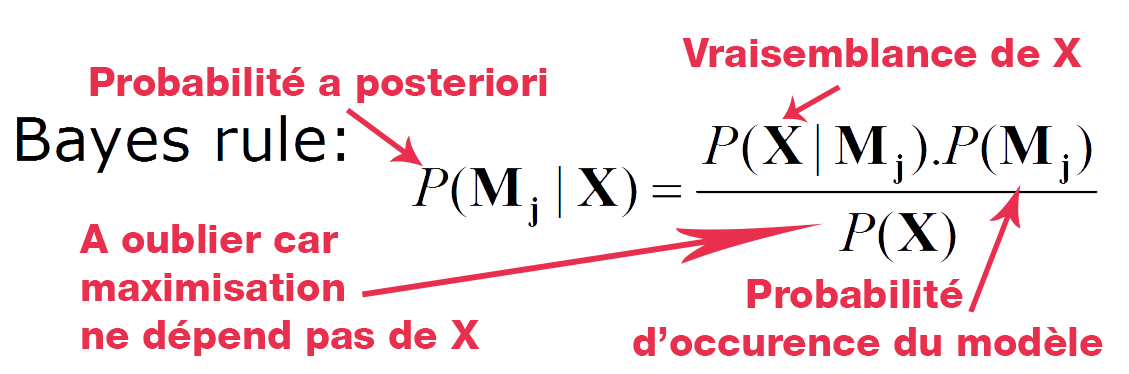
\includegraphics[scale=0.4]{Images/bayes}
				\end{figure}\noindent
			\end{minipage}
		%
		\paragraph{\red{Développer la règle de Bayes afin d'obtenir une expression exploitable de la probabilité 
		~\\ \hspace*{0.035cm} à posteriori de prononciation d'une phrase, justifier chaque étape de ce
		développement.}}~\\
			\begin{figure}[H]
				\centering
				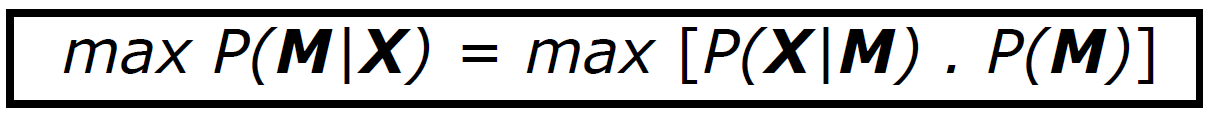
\includegraphics[scale=0.3]{Images/bayes1_5}
			\end{figure}\noindent
			\begin{minipage}{0.4\textwidth}
				La vraisemblance de X se calcule selon le nombre de \hl{transcriptions possibles} (façon de dire) du
					modèle et de la probabilité de chaque transcription ($P(P_i|M)$). $P_i$ = suite de phonèmes.
			\end{minipage}\hfill
			\begin{minipage}{0.55\textwidth}
				\begin{figure}[H]
					\centering
					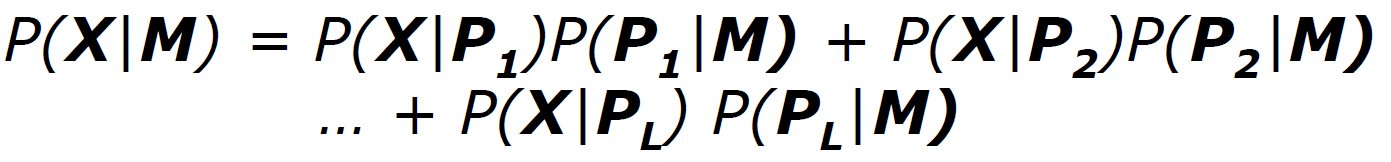
\includegraphics[scale=0.25]{Images/bayes2}
				\end{figure}\noindent
			\end{minipage}
		%
		\paragraph{\red{Citer les probabilités estimées par les modèles acoustique, phonétique et de la langue.}}
		~\\
			\vspace*{-0.4cm}
			\begin{figure}[H]
				\centering
				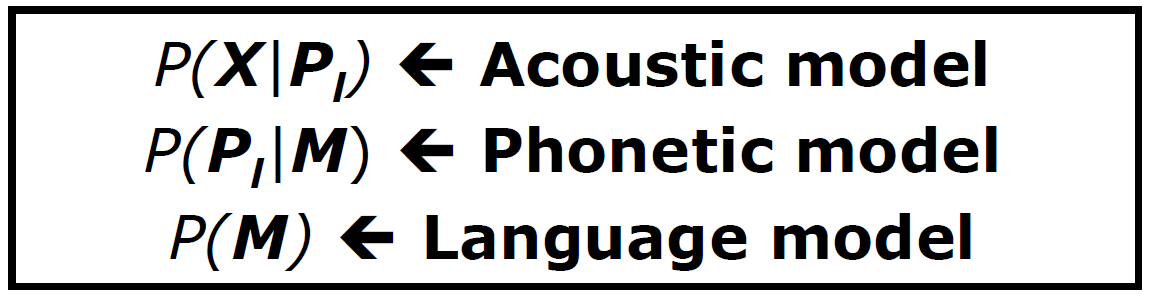
\includegraphics[scale=0.2]{Images/bayes3}
			\end{figure}\noindent
		%
	\subsection{Acoustic Model : Markov Chain}
		\paragraph{\red{Décrire le principe des chaînes de Markov.}}~\\~\\
			\begin{minipage}{0.4\textwidth}
				\begin{figure}[H]
					\centering
					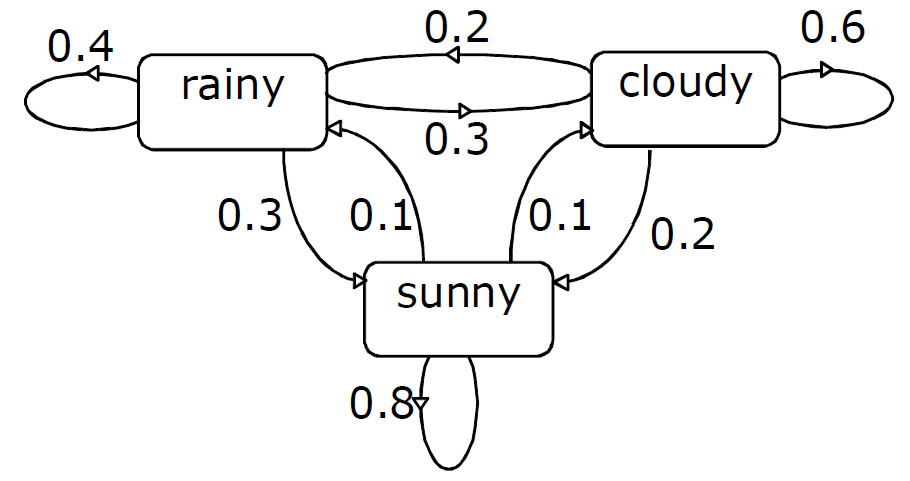
\includegraphics[scale=0.225]{Images/markov_chain}
				\end{figure}\noindent
			\end{minipage}\hfill
			\begin{minipage}{0.55\textwidth}
				\point \hl{Automate} déterministe fini et stochastique avec des probabilités liés à la 
					transition entre ces états. Une suite de phonème pourrait être suivie dans un tel modèle.\\
				\point \myul{Problème} : Il y a plusieurs suites de phonèmes possible pour exprimer la même chose.
			\end{minipage}
		%
		\paragraph{\red{Expliquer pourquoi une chaîne de Markov ne permet pas de calculer directement une 
		~\\ \hspace*{0.035cm} probabilité dans un modèle acoustique en reconnaissance de parole basée sur des 
		~\\ \hspace*{0.035cm} exemples.}}~\\
			\point Dans le modèle de Markov, la probabilité d'un état donné dépend uniquement de la  
				\\\alinea probabilité de la transition vers lui depuis l'état précédent. 
				\\\alinea De plus, l'ensemble des états est observable, il n'y a aucune indétermination 
				\\\alinea sur ces états.\\
			\point Or, le signal de parole est constitué de phonème, et la coarticulation fait qu'il n'est pas
				\\\alinea possible de savoir avec précision quel son a voulu être prononcé ($\rightarrow$ \hl{pas 
				observable})\\\alinea De plus, il existe \hl{plusieurs fa\c con de prononcer} une même phrase et 
				un exemple devrait \\\alinea donc avoir plusieurs chaînes de Markov qui lui est associé.
		
		%
	\subsection{Acoustic Model : Hidden Markov Model (HMM)}
		\paragraph{\red{Décrire le fonctionnement des modèles de Markov cachés sur base d'un exemple.}}~\\~\\
			\begin{minipage}{0.4\textwidth}
				\point On a trois boites avec des boules de couleurs différentes. On peut donc calculer la 
					probabilité d'aller chercher une boule d'une certaine couleur selon ce qui a déjà été pris.
			\end{minipage}\hfill
			\begin{minipage}{0.55\textwidth}
				\begin{figure}[H]
					\centering
					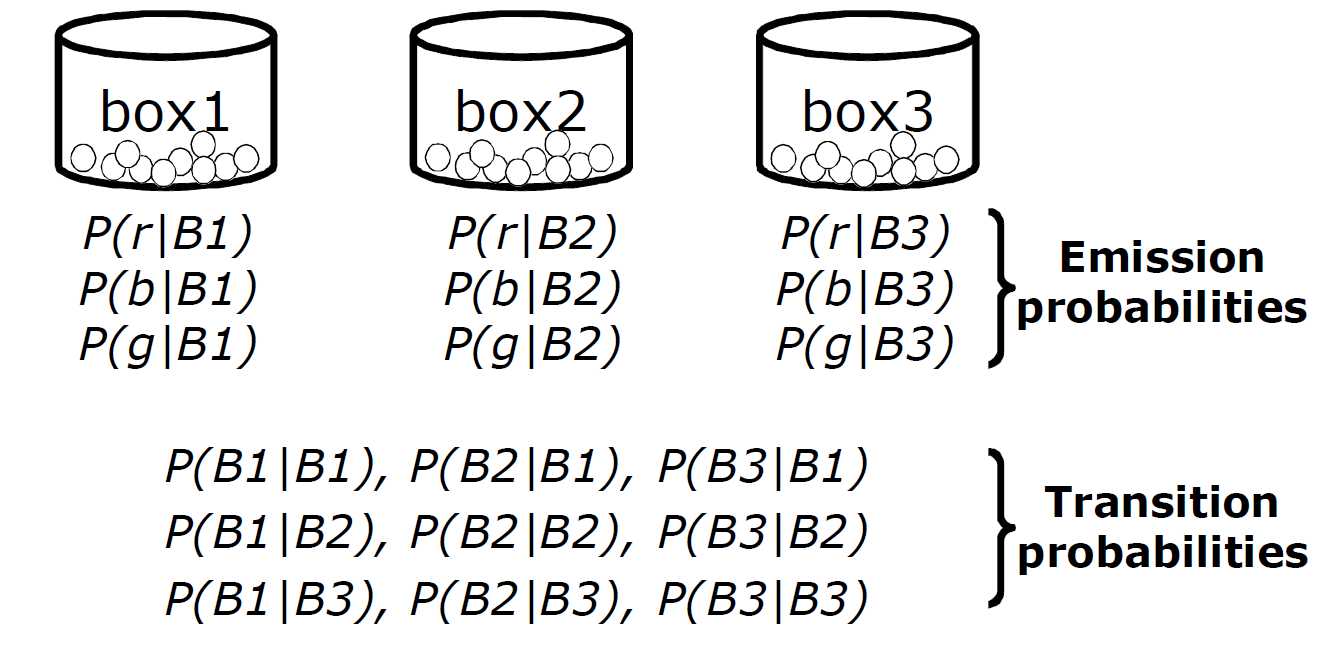
\includegraphics[scale=0.245]{Images/hmm}
				\end{figure}\noindent
			\end{minipage}~\\
			\begin{minipage}{0.4\textwidth}
				\begin{figure}[H]
					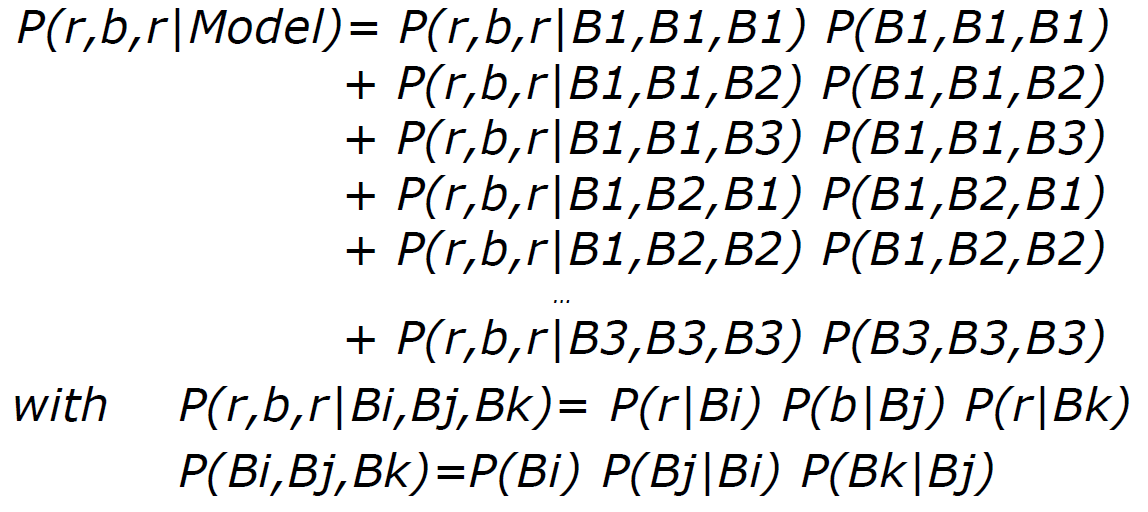
\includegraphics[scale=0.3]{Images/hmm2}
				\end{figure}\noindent
			\end{minipage}\hfill
			\begin{minipage}{0.55\textwidth}
				\point On a donc un grand nombre de combinaison qui rendent la suite "rouge, bleu, rouge" 
					possible.\\~\\
				\point Mais, l'expérimentateur peut décider à tout moment de changer de boite. On veut donc savoir
					la probabilité d'une suite de couleur étant donné cette \textit{\hl{double ind\'etermination}}.
			\end{minipage}
		%
		\paragraph{\red{Différencier les probabilités d'émission et de transition dans les modèles de Markov cachés.}}
		~\\
			\point \myul{Probabilité d'émission} : probabilité qu'un évènement se produise dans un état.
				\\\alinea $\rightarrow$ Probabilité d'une couleur prise dans une boite donnée.\\
			\point \myul{Probabilité de transition} : probabilité qu'une transition d'état se produise.
				\\\alinea $\rightarrow$ Probabilité que l'on change de boite pour prendre une boule.
		%
		\paragraph{\red{Définir en quoi les modèles de Markov cachés sont-ils doublement stochastiques.}}~\\~\\
			\point Pour l'exemple, on doit jouer à la fois sur l'inconnue couleur mais aussi sur l'inconnue 
				\\\alinea boite choisie. On doit donc prendre en compte les probabilités d'émission et les 
				\\\alinea probabilités de transition.
		%
		\paragraph{\red{Citer et définir les trois types de problèmes à traiter pour utiliser les modèles de 
		~\\ \hspace*{0.035cm} Markov cachés.}}~\\
			\vspace*{-0.45cm}
			\begin{itemize}
				\setlength{\itemsep}{0pt}		
				\setlength{\parskip}{0pt}		
				\setlength{\parsep}{0pt}	
				\item \myul{Estimation}: quelle est la \hl{probabilit\'e de l'occurrence} des données 
					étant donné le modèle.
				\item \myul{Entraînement}: comment calculer les \hl{probabilit\'e d'\'emission et de transition}.
				\item \myul{Décodage}: étant donné une séquence d'observations (boules), 
					quelle est la \hl{suite d'\'etats} (boite) \hl{la plus probable} qui mène à cette séquence 
					d'observation.
			\end{itemize}
		%
		\paragraph{\red{Citer les deux algorithmes utilisés pour résoudre le problème d'estimation des modèles 
		~\\ \hspace*{0.035cm} de Markov cachés.}}~\\
			\vspace*{-0.45cm}
			\begin{itemize}
				\setlength{\itemsep}{0pt}		
				\setlength{\parskip}{0pt}		
				\setlength{\parsep}{0pt}	
				\item \myul{Baum-Welch}: prend en compte \hl{tous les chemins possibles} dans le calcul.
				\item \myul{Viterbi}: approxime le calcul de probabilité en ne prenant compte que du \hl{chemin 
					le plus probable}.
			\end{itemize}		
		%
		\paragraph{\red{Illustrer par un exemple l'entraînement d'un modèle de Markov caché.}}~\\~\\
			Sur l'exemple des boules et des boites : 
			\begin{enumerate}
				\setlength{\itemsep}{0pt}		
				\setlength{\parskip}{0pt}		
				\setlength{\parsep}{0pt}	
				\item On prend une longue séquence de boules.
				\item On suppose qu'on connait les probabilités d'émission et de transition, et si on ne les 
					connaît pas, on les invente au hasard.
				\item On décode la séquence $\rightarrow$ On estime de quelle boite provient une boule de la 
					séquence.
				\item On ré-estime les probabilités d'émission et de transition
			\end{enumerate}
			On répète jusqu'à stabilisation du système (les probabilités ne changent plus entre deux itérations).
		%
		\paragraph{\red{Énoncer le principe général de l'algorithme EM permettant l'entraînement des modèles de 
		~\\ \hspace*{0.035cm} Markov cachés.}}~\\
			\vspace*{-0.45cm}
			\begin{enumerate}
				\setlength{\itemsep}{0pt}		
				\setlength{\parskip}{0pt}		
				\setlength{\parsep}{0pt}	
				\item On prend une longue séquence de données sur lesquelles travailler.
				\item On \hl{suppose qu'on connait les probabilit\'es} d'émission et de transition, et si on ne les 
					connaît pas, on les invente au hasard.
				\item On \hl{d\'ecode} la séquence $\rightarrow$ On estime de quelle état provient un élément de la 
					séquence.
				\item On \hl{r\'e-estime les probabilit\'es} d'émission et de transition
			\end{enumerate}
			On répète \hl{jusqu'\`a stabilisation} du système
		%
	\subsection{Phonetic Model}
		\paragraph{\red{Citer la technique utilisée dans les modèles phonétique pour calculer la probabilité 
		~\\ \hspace*{0.035cm} d'une transcription phonétique étant donné une suite de mots.}}~\\~\\
			\point On utilise des \hl{cha\^ines de Markov}. Chaque état de l'automate est lui même un automate 
				\\\alinea 
		%
		\paragraph{\red{Donner un exemple illustrant les limites des modèles phonétiques.}}~\\
			\begin{minipage}{0.66\textwidth}
				\point On ne travaille qu'avec des \hl{probabilit\'es a priori}, on ne tient pas compte du mot qui
				suit. Ce qui biaise les résultats de ces modèles.
			\end{minipage}\hfill
			\begin{minipage}{0.275\textwidth}
				\begin{figure}[H]
					\centering
					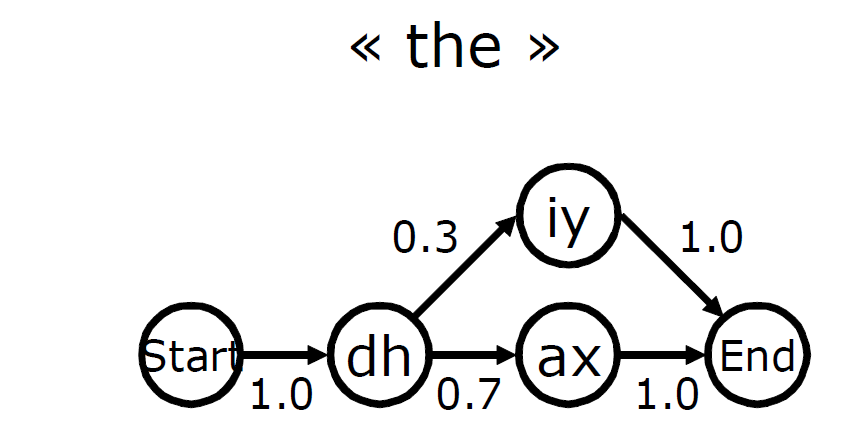
\includegraphics[scale=0.275]{Images/phonetic_markov}
				\end{figure}\noindent
			\end{minipage}
		%
		\paragraph{\red{Préciser comment les modèles phonétiques intègrent un traitement individualisé pour 
		~\\ \hspace*{0.035cm} chaque phonème et signaler les avantages de cette technique.}}~\\~\\
			\begin{minipage}{0.525\textwidth}
				\point Si \hl{chaque phon\`eme a sa propre cha\^ine de Markov}, la chaîne de Markov du mot 
					devient alors un Markov caché.\\
				\point Le but d'une telle pratique est de permettre à un modèle une très grande diversité en
					n'utilisant qu'un seul grand modèle, ce qui permet de réaliser en une fois l'entrainement
					du modèle.
			\end{minipage}\hfill
			\begin{minipage}{0.45\textwidth}
				\begin{figure}[H]
					\centering
					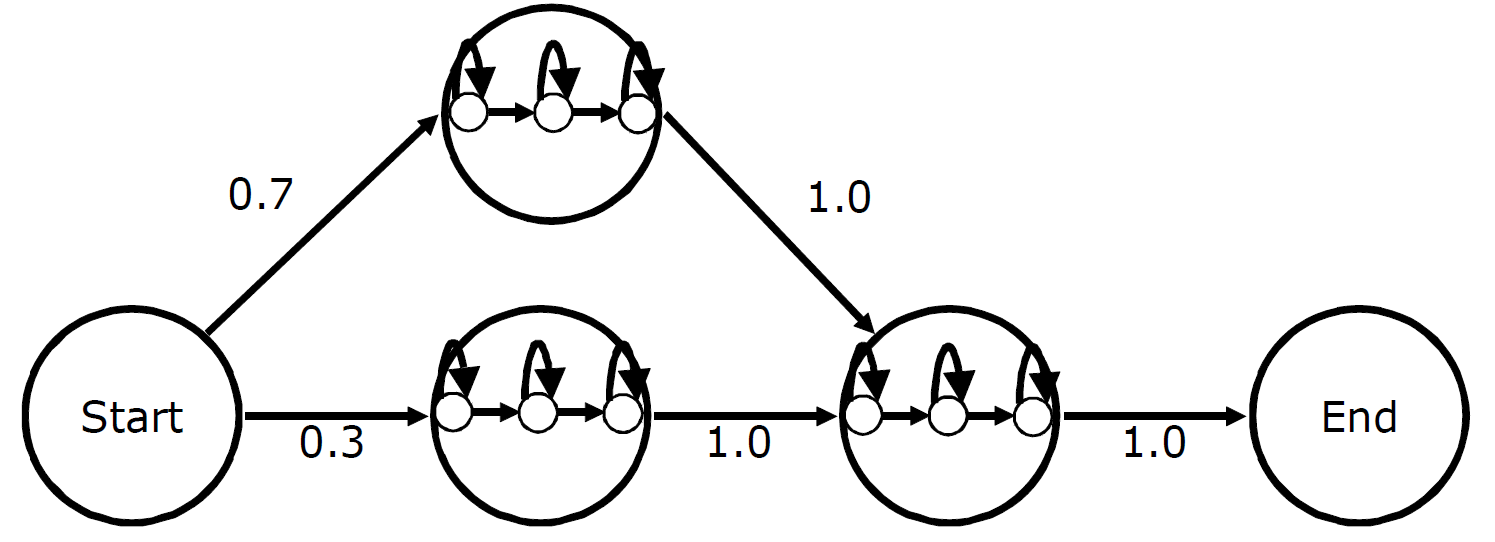
\includegraphics[scale=0.2]{Images/phonetic_hmm}
				\end{figure}\noindent
			\end{minipage}
		%
	\subsection{Language Model}
		%	
		\paragraph{\red{Citer et définir les trois problèmes des modèles de la langue.}}~\\
			\begin{itemize}	
				\item \myul{Entraînement}: comment estimer les valeurs des \hl{param\`etres des mod\`eles}
				\item \myul{Estimation}: comment estimer la probabilité d'une phrase dans la modèle de la
					langue.
				\item \myul{Décodage}: le nombre de phrase d'une langue étant infini, il est impossible de 
					fournir une liste exhaustive de toutes les phrases prononçable. On va donc essayer
					de deviner le mot qui suivra le mot précédent afin d'essayer de discrétiser les cas possibles.
			\end{itemize}
		%
		\paragraph{\red{Exprimer de trois façons différentes la probabilité de prononcer une phrase donnée en 
		~\\ \hspace*{0.035cm} fonction des mots qui la composent et commenter l'utilisation de ces expressions dans 
		~\\ \hspace*{0.035cm} les modèles de la langue.}}~\\
		\begin{minipage}{0.4\textwidth}
			\begin{figure}[H]
				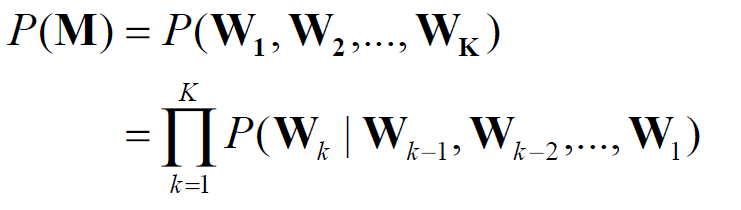
\includegraphics[scale=0.4]{Images/language_model1}
			\end{figure}\noindent
		\end{minipage}\hfill
		\begin{minipage}{0.55\textwidth}
			\point Part du principe que chaque mot permet de \hl{deviner un ensemble de mot qui pourrait le suivre}.\\
			\point Impossible à réaliser dans la réalité...
		\end{minipage}~\\
		\begin{minipage}{0.55\textwidth}
			\point Part du principe que \hl{certains couples de mots reviennent souvent} et que d'\hl{autres} 
				ne veulent rien dire ou sont \hl{tr\`es rare}s.\\
			\point S'entraine à partir d'un très grand corpus de textes. S'estime et se décode grâce
				à une grande base de données dans laquelle le corpus a été entré $\rightarrow$ Tend à
				éliminer des couples considérés comme "improbables" alors qu'ils se retrouvent peut être souvent
				dans le langage parlé.
		\end{minipage}\hfill
		\begin{minipage}{0.4\textwidth}
			\begin{figure}[H]
				\centering
				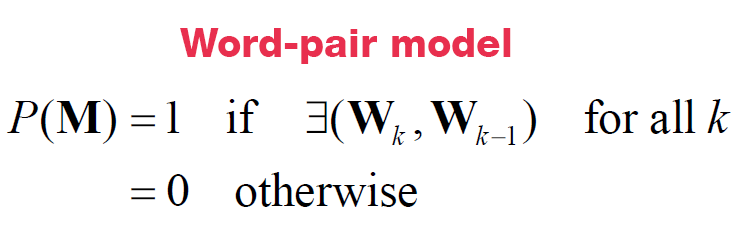
\includegraphics[scale=0.4]{Images/language_model2}
			\end{figure}\noindent
		\end{minipage}~\\
		\begin{minipage}{0.5\textwidth}
			\begin{figure}[H]
				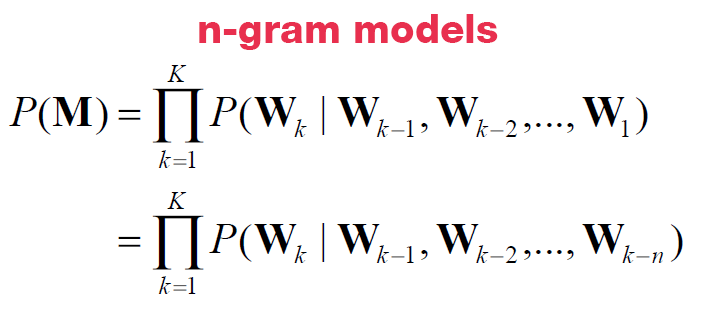
\includegraphics[scale=0.35]{Images/language_model3}
			\end{figure}\noindent
		\end{minipage}\hfill
		\begin{minipage}{0.45\textwidth}
			\point Essaie de \hl{deviner un mot selon les n mots qui le pr\'ec\`ede}. 
				Un tri-gram (n=2) essaie de deviner le mot suivant ses deux prédécesseurs.
		\end{minipage}
		
		%
		\paragraph{\red{Donner une valeur réaliste au nombre n du modèle n-gramme et préciser les conséquences 
		~\\ \hspace*{0.035cm} liées à ce choix.}}~\\~\\
			\point On peut se limiter à des suites de 3 mots. Mais il arrivera de tomber sur une suite de trois
				\\\alinea mots qui existe dans la langue mais qui ne se retrouve dans aucun texte.
		%
		\paragraph{\red{Citer le problème du modèle n-gramme et proposer deux techniques pour le résoudre.}}~\\~\\
			\point Même si on se limite à trois mots, il existera des suites de 3 mots qui sont très rare et qui
				seront donc considérées comme incorrectes.
			\begin{itemize}
				\setlength{\itemsep}{0pt}		
				\setlength{\parskip}{0pt}		
				\setlength{\parsep}{0pt}	
				\item Back-off: un premier principe est alors de retomber sur deux suites de deux mots, que l'on va 
					\hl{pond\'erer} afin de ne pas considérer la suite de mots comme improbable.
				\item Part-of-speech: on se réfère à la \hl{nature syntaxique} des mots précédents plutôt que de la
					suite même des mots.
			\end{itemize}
		%
		\paragraph{\red{Commenter la qualité actuelle des systèmes exploitant les modèles de la langue.}}~\\~\\
			\point Tout le monde sait que les n-gram sont des approches imparfaites. Mais chaque fois qu'on
				a essayé d'aller plus loin, de préciser ces probabilités, on a fait baisser le 
				taux de reconnaissance.
		%
	\subsection{ASR Conclusion}
		%		
		\paragraph{\red{Positionner le taux d'erreur d'un système de reconnaissance de parole en fonction du type 
		~\\ \hspace*{0.035cm} de reconnaissance, de la tâche, de la dépendance du locuteur, de la taille du
		vocabulaire.}}~\\
			\begin{figure}[H]
				\centering
				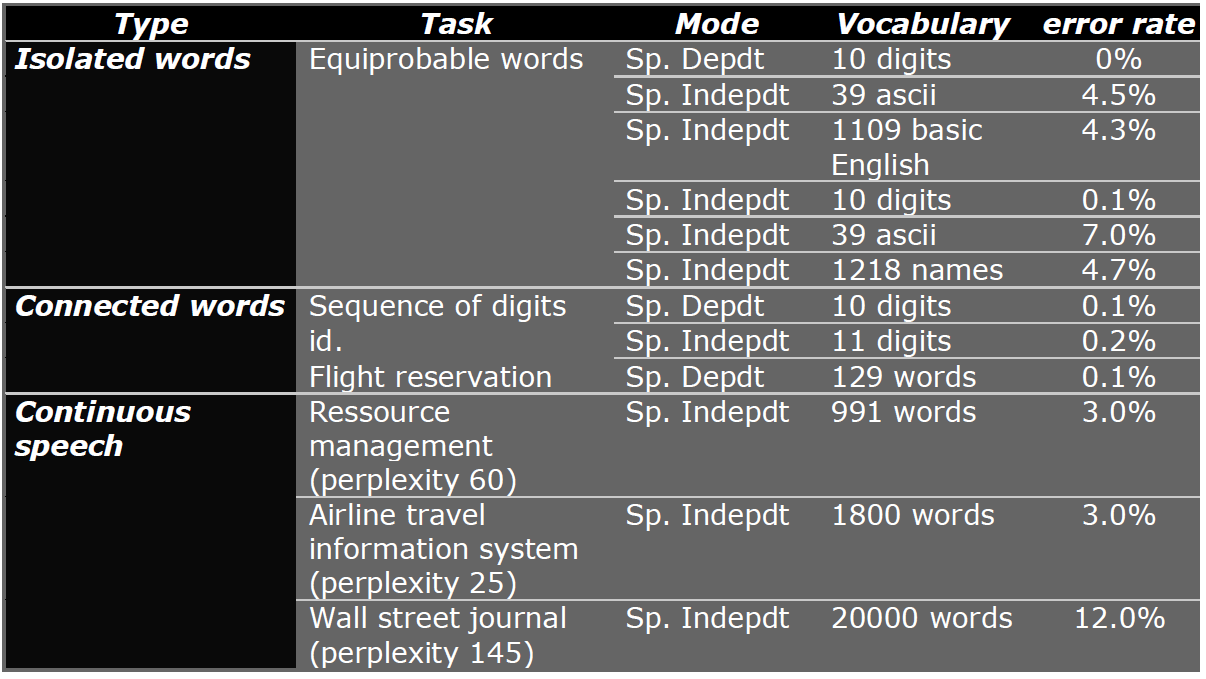
\includegraphics[scale=0.3]{Images/recognition_error}
			\end{figure}\noindent
		
		\paragraph{\red{Expliquer la différence d'erreur de reconnaissance entre la lecture d'un journal en
		~\\ \hspace*{0.035cm} laboratoire et la parole de la vie réelle.}}~\\~\\
			\begin{minipage}{0.4\textwidth}
				\point La parole de la vie réelle comporte du bruit de fond, de bruit gutturaux, de la toux, ...
				 Cela implique un taux d'erreur supplémentaire d'environ 30\%.
			\end{minipage}\hfill
			\begin{minipage}{0.55\textwidth}
				\begin{figure}[H]
					\centering
					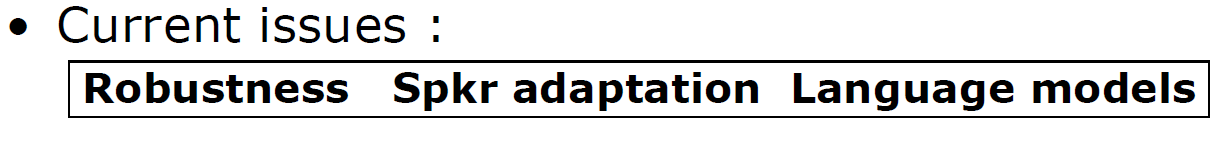
\includegraphics[scale=0.34]{Images/recognition_robustness}
				\end{figure}\noindent
			\end{minipage}
		%	
		\paragraph{\red{Souligner l'importance du modèle de la langue en reconnaissance de parole.}}~\\
			\point Si on fait sauter le modèle de la langue, le taux d'erreur grimpe fortement. Dés lors,
				\\\alinea on peut imaginer grappiller les derniers pourcentages d'erreur en améliorant le
				\\\alinea modèle de la langue.
		%
		\paragraph{\red{Citer les champs d'investigation actuellement explorés en reconnaissance de parole.}}~\\
			\vspace*{-0.45cm}
			\begin{itemize}
				\setlength{\itemsep}{0pt}		
				\setlength{\parskip}{0pt}		
				\setlength{\parsep}{0pt}	
				\item \myul{Robustesse}.
				\item \myul{Modèle de la langue}.
				\item \myul{Adaptation au locuteur} : plus on utilise le système et plus il connait le locuteur 
					et moins il fait d'erreur.
			\end{itemize}
		%
		\paragraph{\red{Justifier qu'un être humain reste plus performant qu'un ordinateur pour reconnaître 
		~\\ \hspace*{0.035cm} la parole.}}~\\~\\
			\point L'être humain est capable à la fois de reconnaître ce qui a été dit mais aussi de 
				\\\alinea comprendre ce qui a été dit. Ce qui est pour le moment assez laborieux pour une machine.\\
			\point On peut donc prévoir que si une machine est capable de comprendre ce qui a été dit, alors,
				\\\alinea le taux d'erreur de reconnaissance de la parole serait facilement diminué.
		%
\pagebreak
\section{Speech Synthesis}
	\subsection{Notes du présentiel}
		\paragraph{\green{Domaines d'application}}~\\~\\
			\point Beaucoup de domaines ont été abandonnés comme le renseignement par téléphone. 
				\\\alinea Le plus gros domaine reste l'aide aux handicapés et la recherche.
		\paragraph{\green{En quoi c'est difficile ? Phonétisation - Intonation - Durée}}~\\~\\
			\point Problèmes liés à la langue (principalement langue française) comme l'homographe hétérogène.
				\\\alinea ce sont des mots qui s'écrivent de la même manière mais se prononcent de manière différente.
				\\\alinea Il y a aussi des assimilations de nasalité (des phonèmes que l'on ne prononce
				\\\alinea pas correctement), ...\\
			\point L'intonation présente des problèmes : comment modéliser une courbe de pitch ? Cette courbe
				\\\alinea est un tout car la moindre modification s'entend, mais chaque personne le dira différemment.
				\\\alinea L'accent tonique est également un problème.\\
			\point La durée d'un même phonème à deux endroit différents d'une phrase n'aura pas du tout
				\\\alinea la même durée.
		\paragraph{\green{En quoi c'est difficile ? Traitement de signal}}~\\~\\
			\point Coarticulation pose un gros problème...
		\paragraph{\green{Historique}}~\\~\\
			\point Première machines parlantes en 1791 et machine mécanique plus tard ... Mais que pour 
				\\\alinea des sons de base.\\
			\point Machine à parler électrique de 1936 avec 10 touches qui représentent les formants et pédale 
				\\\alinea de pitch, etc... C'est bien, mais rien d'automatisé.\\
			\begin{itemize}
			 	\setlength{\itemsep}{0pt}		
			 	\setlength{\parskip}{0pt}		
			 	\setlength{\parsep}{0pt}	
			 	\item Premiers TTS : création de formants.
			 	\item Deuxième type de TTS : On colle des diphones\footnote{Moitié de son (couple de phonème) qui 
					permette de résoudre le problème de coarticulation en coupant le son après la première moitié du 
					premier phonème et avant la deuxième moitié du deuxième phonème} ensemble.
				\item Troisième et dernier type : système automatique à très grande BDD qui cherche les meilleurs
					diphones pour le mot à dire.
			 \end{itemize}
\pagebreak
	\subsection{Text-To-Speech Synthesis}
		\paragraph{\red{Citer trois applications de la synthèse de parole en télécommunication.}}~\\
		\vspace*{-0.66cm}
			\begin{itemize}
				\setlength{\itemsep}{0pt}		
				\setlength{\parskip}{0pt}		
				\setlength{\parsep}{0pt}	
				\item Téléphone
				\item Multimédia
				\item Communication homme-machine
			\end{itemize}
		%
		\paragraph{\red{Positionner le besoin en interactivité pour les applications actuelles en téléphonie.}}~\\~\\
			\point On voudrait savoir qui appelle, avoir assistant virtuel, annuaire inversé, ou encore
				\\\alinea avoir accès à des informations par une demande vocale	(application obsolète aujourd'hui).
		%
		\paragraph{\red{Donner un exemple d'application de la synthèse de parole dans le domaine du multimédia.}}
		~\\
			\point Jeux interactifs, livre parlant, ...
		%
		\paragraph{\red{Justifier l'intérêt de la synthèse de parole pour la communication homme-machine.}}~\\~\\
			\point Pouvoir contrôler, ou du moins communiquer avec des machines avancées.
		%
		\paragraph{\red{Préciser en quoi la synthèse de parole apporte une aide aux handicapés.}}~\\~\\
			\point C'est le domaine d'application le plus touché par la synthèse de la parole. Ces systèmes
				\\\alinea permettent aux personnes dans l'incapacité de parler de communiquer.
		%
		\paragraph{\red{Expliquer pourquoi la synthèse de parole est d'une importance fondamentale pour les
		~\\ \hspace*{0.035cm} expériences scientifiques sur le langage naturel.}}~\\~\\
			\point Elle permet de mieux comprendre la façon dont nous parlons.
		%
	\subsection{TTS Diagram / Phonetization}
		
		\paragraph{\red{Schématiser un synthétiseur de parole TTS.}}~\\
			\begin{figure}[H]
				\centering
				\includegraphics[scale=0.43]{Images/tts}
			\end{figure}\noindent		
		%
		\paragraph{\red{Définir le rôle des linguistes informaticiens.}}~\\~\\
			\point \'Etablir un pont entre le traitement du langage naturel et les applications informatiques.
				\\\alinea en utilisant les règles et connaissances des linguistes, ils s'occupent du passage 
				\\\alinea de (a) et (b) à (c).
		%
		\paragraph{\red{Identifier la première difficulté de l'étape de phonétisation et présenter quatre 
		~\\ \hspace*{0.035cm} exemples supplémentaires de difficultés illustrant la complexité de cette étape.}}~\\~\\
			\point On pourrait penser qu'il suffit de transformer tous les lettres présentes dans le texte 
					\\\alinea en phonèmes, mais on trouve alors plusieurs problèmes.\\~\\
			\begin{minipage}{0.4\textwidth}
				\begin{itemize}
					\setlength{\itemsep}{0pt}		
					\setlength{\parskip}{0pt}		
					\setlength{\parsep}{0pt}	
					\item \myul{Homographes-Hétérophones}: mots s'écrivant de la même manière mais se 
						\hl{pronon\c cant diff\'eremment}.
					\item \myul{Les liaisons phonétiques}: certaines \hl{liaisons} sont \hl{obligatoires}, 
						d'autres facultatives, et d'autres interdites
					\item \myul{Assimilation de nasalité}: phonèmes qui sonnent différemment selon les phonèmes qui
						le précèdent ou qui le suivent (\hl{contraintes physiques des cordes vocales}).
				\end{itemize}
			\end{minipage}\hfill
			\begin{minipage}{0.55\textwidth}
				\begin{figure}[H]
					\includegraphics[scale=0.5]{Images/phonetization}
				\end{figure}\noindent
			\end{minipage}~\\
			\point \`A noter qu'il n'est pas nécessaire de comprendre la phrase pour pouvoir la phonétiser;
				\\\alinea L'exemple de M. Lewis le prouve.
		%
	\subsection{Intonation / Coarticulation}
		\paragraph{\red{Préciser l'utilité des fréquents mouvements intonatifs dans le langage naturel.}}~\\~\\
    		\point Ils permettent au receveur de bien séparer les groupes de mots que l'envoyeur prononce.
    	%
    	\paragraph{\red{Préciser le problème rencontré lors de la modification artificielle de la courbe 
    	~\\ \hspace*{0.035cm} intonative.}}~\\~\\
			\point La courbe représente un tout, le moindre changement pourrait rendre toute la courbe invalide.
				\\\alinea Cependant, la même phrase ne sera jamais prononcée deux fois avec la même courbe de pitch.
		%
		\paragraph{\red{Citer les deux autres rôles majeurs de l'intonation.}}~\\
			\vspace*{-0.5cm}
			\begin{itemize}
				\setlength{\itemsep}{0pt}		
				\setlength{\parskip}{0pt}		
				\setlength{\parsep}{0pt}	
				\item Mettre en évidence certains mots $\rightarrow$ Porter une information différente.
				\item Permettre à l'auditeur de savoir quand la phrase est terminée.
			\end{itemize}		
		%
		\paragraph{\red{Caractériser les durées des phonèmes.}}~\\~\\
			\point \hl{Non constante}, et différente selon la position du phonème dans la phrase et même dans
				\\\alinea le mot. Elle est donc liée à l'intonation et est assez compliquée à formaliser.
				\\\alinea Pour les voyelles, cette durée est corrélée avec la fréquence fondamentale.
		%
		\paragraph{\red{Citer les connaissances nécessaires pour appliquer une intonation à une phrase.}}~\\
			\vspace*{-0.5cm}
			\begin{itemize}
				\setlength{\itemsep}{0pt}		
				\setlength{\parskip}{0pt}		
				\setlength{\parsep}{0pt}	
				\item \myul{Syntaxe}: connaître la \hl{nature du mot} et sa position permet d'avoir beaucoup 
					d'information sur le mot, y comprit sa phonétisation, intonation et durée.
				\item \myul{Sémantique}: \hl{comprendre} la phrase permet de compléter la connaissance.
				\item \myul{Pragmatique}: sens \hl{sous-entendu} dans la phrase par l'intonation par exemple.
			\end{itemize}
    	%
		\paragraph{\red{Justifier que la synthèse de parole tente de reproduire la coarticulation.}}~\\~\\
			\point Chaque phonème se prononçant différemment et à une vitesse différente, \hl{on ne sait pas}
				\\\alinea \hl{d\'efinir un unique son par phon\`eme}. Dés lors, il faut pouvoir imiter ces
					 différences.
		%
		\paragraph{\red{Résumer les défis et contraintes auxquels doit répondre la synthèse de parole.}}~\\
			\vspace*{-0.5cm}
			\begin{itemize}
				\setlength{\itemsep}{0pt}		
				\setlength{\parskip}{0pt}		
				\setlength{\parsep}{0pt}	
				\item Phonétisation correcte.
				\item Générer une prosodie (intonation et durée et le rythme);
				\item Produire une suite de phonème coarticulés.
				\item Contraintes de coût, de maintenance, de calcul et d'adaptation à la langue.
			\end{itemize}
		%
	\subsection{TTS techniques}
		\paragraph{\red{Résumer le principe de fonctionnement de la machine de Von Kempelen.}}~\\~\\
			\point On simule l'appareil vocale dans une machine mécanique avec un souffleur, une hanche
				\\\alinea (pour simuler les cordes vocales), une bouche molle et un souffleur permettant
				\\\alinea les explosions de certains phonèmes.
		%
		\paragraph{\red{Résumer le principe de fonctionnement du Voder d'Omer Dudley.}}~\\~\\
    		\point Cette fois ci, un opérateur a accès à un clavier composé de 10 touches, et de plusieurs
    			\\\alinea autres clapets supplémentaires (pitch, énergie, ...). On peut faire le rapprochement
    			\\\alinea entre les 10 paramètres du modèle LPC mais en analogique.
    	%
    	\paragraph{\red{Exposer l'idée de la synthèse par formants et justifier son nom.}}~\\
			\point Comme certains spécialistes savent lire des spectrogramme, l'idée est de formaliser cette
				\\\alinea expertise, inversée, dans le synthétiseur pour qu'il puisse créer les formants
				\\\alinea correspondant au mot à prononcer.
		%
		\paragraph{\red{Caractériser la parole générée lors d'une synthèse par formants.}}~\\
			\point Métallique et entrecoupée. Tout sauf naturel. Néanmoins utilisée par les handicapés à l'époque.
		%
	\subsection{Diphone / Unit selection-based synthesis}
		\paragraph{\red{Énoncer le principe de fonctionnement de la synthèse par diphone.}}~\\
			\point On colle des diphones\footnote{Moitié de son (couple de phonèmes) qui 
					embarque en son sein l'essentiel de la coarticulation entre les deux sons et s'obtient en 
					coupant le son après la première 
					moitié du premier phonème et avant la deuxième moitié du deuxième phonème} ensemble.
		%
		\paragraph{\red{Préciser comment la synthèse par diphone respecte la coarticulation du langage naturel.}}
		~\\~\\
			\point Un système de modification de prosodie va permettre de retrouver au mieux l'intonation  
				\\\alinea et la durée du signal. Et un système de lissage va permettre de lier au mieux les 
				\\\alinea diphones entre eux.
		%
		\paragraph{\red{ Schématiser le fonctionnement d'un synthétiseur de parole par diphone et préciser 
		~\\ \hspace*{0.035cm} sur ce schéma les deux principaux problèmes du modèle.}}~\\
			\begin{figure}[H]
				\centering
				\includegraphics[scale=0.5]{Images/diphone}
			\end{figure}\noindent
		%
		\paragraph{\red{Commenter le développement du projet MBROLA.}}~\\
			\point Part du principe de PSOLA qui avait comme idée que coller à des endroits différents que  
				\\\alinea la base des fenêtres (en cloche) de pondérations lors de l'analyse.
				\\\alinea Il a été développé par M. Dutoit dans le cadre de son doctorat
		%
		\paragraph{\red{Citer la différence entre la synthèse par sélection d'unité et la synthèse par diphone.}}
		~\\~\\
			\begin{minipage}{0.4\textwidth}
				\point Cette technique nécessite une \hl{grande base de donn\'ee} contenant plusieurs fois tous 
					les diphones. Avec cette base, le principe est de rechercher les \hl{meilleurs diphones}
					de la BDD en prenant en compte le diphone précédant et suivant le diphone recherché.
			\end{minipage}\hfill
			\begin{minipage}{0.55\textwidth}
				\begin{figure}[H]
					\centering
					\includegraphics[scale=0.425]{Images/automatic_diphone}
				\end{figure}\noindent
			\end{minipage}
		%
		\vspace*{-0.65cm}
		\paragraph{\red{Citer le problème qu'il restait à résoudre en synthèse par sélection d'unité.}}~\\
    		\point La recherche des meilleurs diphones dans la base de données.
    	%
    \subsection{Pre-processing / Morphological analysis / Contextual analysis}
    	\paragraph{\red{Citer les sous-modules d'un module de traitement du langage naturel dans un système 
    	~\\ \hspace*{0.035cm} de synthèse de parole.}}~\\
			\begin{figure}[H]
				\centering
				\includegraphics[scale=0.45]{Images/phonetics}
			\end{figure}\noindent
		%
		\vspace*{-0.75cm}
		\paragraph{\red{Citer les rôles du prétraitement dans un système de synthèse de parole.}}~\\
			\begin{itemize}
				\setlength{\itemsep}{0pt}		
				\setlength{\parskip}{0pt}		
				\setlength{\parsep}{0pt}	
				\item Détecter les nombres
				\item Détecter les acronymes
				\item Détecter les abréviations
				\item Détecter quel \hl{"."} termine la phrase et lesquelles ne la termine pas.
			\end{itemize}
		%
		\paragraph{\red{Citer le type d'outils généralement utilisés pour résoudre une grande partie des 
		~\\ \hspace*{0.035cm} problèmes de prétraitement en synthèse de parole.}}~\\~\\
			\point \hl{Grammaires} régulières simples à états finis.
		%
		\vspace*{-0.75cm}
		\paragraph{\red{Justifier l'utilité de l'analyse morphologique en synthèse de parole.}}~\\
			 \begin{itemize}
			 	\setlength{\itemsep}{0pt}		
			 	\setlength{\parskip}{0pt}		
			 	\setlength{\parsep}{0pt}	
			 	\item Réduire la taille du lexique (grâce aux préfixes commun et suffixes circonstanciels).
			 	\item Aider à la prononciation lorsque la morphologie y est liée.
			 	\item Préciser les différentes natures possibles pour un même mot.
			 	\item Savoir quand l'accent tonique tombe dans un mot.
			 \end{itemize}
		%
		\paragraph{\red{Préciser comment est réalisée l'analyse morphologique en synthèse de parole.}}~\\~\\
			\point Règles régulières, \hl{automates} à états finis. Dans tous les cas, c'est très dépendant 
				\\\alinea de la langue. On peut aussi utiliser une brute force sur un dictionnaire.
		%
		\paragraph{\red{Énoncer le but de l'analyse contextuelle et exposer la méthode pour y parvenir.}}~\\~\\
			\begin{minipage}{0.4\textwidth}
				\point Le but est de trouver quel morphologie chaque mot a dans une phrase précise. Donc de
					\hl{trouver le chemin} parmis un graphe contenant toutes les natures possibles du mot.\\
				\point Pour ce faire, on va utiliser la technique des \hl{n-grammes} (voir partie 4 : ASR). 
					C'est donc des modè-les probabilistes qui permettront de décider du meilleur chemin.
			\end{minipage}\hfill
			\begin{minipage}{0.55\textwidth}
				\begin{figure}[H]
					\centering
					\includegraphics[scale=0.5]{Images/contextual}
				\end{figure}\noindent
			\end{minipage}
		%
	\subsection{Syntactic-Prosodic Phrasing / Automatic Phonetization}
		\paragraph{\red{Offrir deux solutions pour identifier les groupes de mots d'une phrase en synthèse 
		~\\ \hspace*{0.035cm} de parole.}}~\\
			\vspace*{-0.5cm}
			\begin{itemize}
				\setlength{\itemsep}{0pt}		
				\setlength{\parskip}{0pt}		
				\setlength{\parsep}{0pt}	
				\item Chinks'n chunks : un groupe de mot est composé de chinks suivi de chunks puis s'arrête 
					pour que le prochain groupe commence avec un chink. \myul{\hl{Chink}}: mots fonctionnels.
					\myul{\hl{Chunk}}: mots lexicaux (noms, adjectifs, adverbes adjectivaux, ...).
				\item Les arbres CART : système de Machine-Learning qu'il faut entraîner avec des exemples.
			\end{itemize}
		%
		\paragraph{\red{Spécifier la méthode généralement employée pour réaliser la phonétisation automatique
		~\\ \hspace*{0.035cm} des mots en synthèse de parole et illustrer cette méthode par un exemple.}}~\\~\\
    		\begin{minipage}{0.4\textwidth}
    			\point \hl{R\`egles r\'eguli\'eres} permettant de déclarer tous les cas particuliers, puis généraux.
    				Un graphème  est prononcé [...] quand / il est situé \_.
    		\end{minipage}\hfill
    		\begin{minipage}{0.55\textwidth}
    			\begin{figure}[H]
    				\centering
    				\includegraphics[scale=0.5]{Images/phonetization2}
    			\end{figure}\noindent
    		\end{minipage}
    	%
    	\paragraph{\red{Présenter l'alternative à la méthode habituelle de phonétisation automatique et 
    	~\\ \hspace*{0.035cm} indiquer le point commun entre les deux méthodes.}}~\\~\\
			\begin{minipage}{0.4\textwidth}
				\point Arbre de décision "\hl{TRIE}" qui peuvent être entrainés par une batterie d'exemple.
					Pour que ca puisse fonctionner, comme pour les règles, il faut mettre des règles particulières
					sur la catégorie syntaxique du mot traité.
			\end{minipage}\hfill
			\begin{minipage}{0.55\textwidth}
				\begin{figure}[H]
					\centering
					\includegraphics[scale=0.5]{Images/trie}
				\end{figure}\noindent
			\end{minipage}
		%
	\subsection{Prosody generation}
		\paragraph{\red{Commenter les premiers efforts réalisés pour générer la prosodie en synthèse de parole.}}
		~\\~\\
			\point Consiste en 10 intonations différentes qui permettrait de pouvoir former n'importe quelle
				\\\alinea phrase dans la langue française en les combinant. Le problème est qu'on a jamais
				\\\alinea su mettre des règles sur quelle intonation utiliser à quel moment.
		%
		\paragraph{\red{Définir ce qu'est un ton et spécifier son utilisation pour caractériser un corpus.}}~\\~\\
			\point \myul{Ton}: mouvement voulu associé à la voyelle de chaque syllabe.\\
			\point L'idée est d'associer ces tons aux pics d'intonation présents dans une phrase afin de ne 
				\\\alinea plus avoir à lire la courbe, mais juste ces unités abstraites que sont les tons.
		%
		\paragraph{\red{Déterminer comment générer des tons sur base d'un texte.}}~\\
			\begin{figure}[H]
				\centering
				\includegraphics[scale=0.425]{Images/tones}
			\end{figure}\noindent
		%
		\paragraph{\red{Déterminer comment générer par règles une courbe intonative sur base de tons.}}~\\
			\begin{minipage}{0.4\textwidth}
				\point Part du principe que quelque soit la phrase, il y a toujours une pente descendante.
			\end{minipage}\hfill
			\begin{minipage}{0.55\textwidth}
				\begin{figure}[H]
					\centering
					\includegraphics[scale=0.425]{Images/tones_rules}
				\end{figure}\noindent
			\end{minipage}
		%
		\paragraph{\red{Déterminer comment générer par entraînement une courbe intonative sur base de tons.}}~\\~\\
			\point On a une très grande base de donnée avec des phrases annotées en tons. On entraine
				\\\alinea le système avec cette base de données, et le système s'occupe ensuite de
				\\\alinea décider de la meilleure courbe possible pour la demande, à la fois pour
				\\\alinea l'intonation mais aussi pour éviter les discontinuations d'intonation.
		%
		\paragraph{\red{Établir l'analogie entre la génération de prosodie par entraînement et la synthèse 
		~\\ \hspace*{0.035cm} par sélection d'unité et l'illustrer en schématisant un exemple.}}~\\~\\
			\point Là où la synthèse par selection d'unité colle des diphones entre eux en maximisant
				\\\alinea le match et en minimisant les discontinuités, la génération de prosodie va
				\\\alinea coller des morceaux de sa base de données pour construire une courbe de pitch
				\\\alinea avec les même contraintes.
		%
	\subsection{TTS Conclusion}
		\paragraph{\red{Résumer la tendance suivie depuis 1995 en synthèse de parole et donner une 
		~\\ \hspace*{0.035cm} justification technique à cette tendance.}}~\\~\\
			\point L'idée de machine learning sur corpus et de sélection automatique est à la mode depuis
				\\\alinea 1995, donc depuis l'explosion de la taille des médias numériques.
				\\\alinea Plus récemment, ce sont les réseaux de neurones profonds qui prennent le dessus dans 
				\\\alinea la recherche. Ceux-ci ont l'inconvénient d'être très complexe et on a pas beaucoup
				\\\alinea de contrôles sur les résultats de ceux-ci.
		%
\pagebreak
\section{Conclusion on Speech Processing}
		\paragraph{\red{ Positionner l'évolution du codage de parole à l'heure actuelle.}}~\\~\\
			\point On a presque trouvé tout ce qui pouvait être trouvé $\rightarrow$ On connait les normes.
		%
		\paragraph{\red{Positionner l'évolution de la reconnaissance de parole à l'heure actuelle.}}~\\~\\
			\point Il y a des systèmes ouverts pour le grand public, mais avec toujours les problèmes de 
				\\\alinea robustesse, de non-compréhension, ... Ceci s'est amélioré depuis 2003 mais il reste
				\\\alinea du travail.
		%
		\paragraph{\red{Positionner l'évolution de la synthèse de parole à l'heure actuelle et la comparer à 
		~\\ \hspace*{0.035cm} celle de la reconnaissance de parole.}}~\\~\\
			\point Les résultats sont très bons mais on peut faire encore mieux.
		%
		\paragraph{\red{ Souligner l'importance qu'ont prise les grandes bases de données de parole dans le 
		~\\ \hspace*{0.035cm} domaine du traitement de parole.}}~\\~\\
			\point Les systèmes de Machine-Learning demandent de grands corpus. On en dispose maintenant
				\\\alinea de très grandes étiquetées en intonation, en nature de mots, ...
				\\\alinea Les bases de données sont généralement centralisées dans un laboratoire et on
				\\\alinea y a accès soit moyennant paiement, soit librement auprès de laboratoires.
				\\\alinea Il y a autant de données audio que de texte dans ces bases de données.
		%
		\paragraph{\red{Prédire l'avenir des scientifiques de la parole.}}~\\~\\
			\point Se baser de moins en moins sur des règles formelles et de plus en plus sur de l'apprentissage
				\\\alinea automatique. Et sinon, on a besoin de technique d'ingénierie logicielle afin de
				\\\alinea mélanger les parties des différents spécialistes, car il est impossible 
				\\\alinea d'être spécialiste dans tous les domaines de la parole en même temps.
		%
		\paragraph{\red{Émettre un avis critique sur le traitement de la parole.}}~\\~\\
			\point It's up to you folks !
		%
\end{document}